\documentclass[11pt]{article}

% Default margins are too wide all the way around. I reset them here

\usepackage[a4paper,
			twoside,
			left=1.5in,
			right=1.0in,
			textheight=9in, 
			headheight=14pt]{geometry}
			
\usepackage[utf8]{inputenc}
\usepackage[T1]{fontenc}
\usepackage{lmodern}
\usepackage[danish,english]{babel}
\usepackage{setspace}
\usepackage[pdfborder={0 0 0}]{hyperref}

\usepackage{amsmath}
\usepackage{amsfonts}
\usepackage{amssymb}
\usepackage{graphicx}
\usepackage{csquotes}
\usepackage{appendix}
\usepackage[backend=biber, style=apa, sorting=nyt]{biblatex}
\usepackage{algorithm}
\usepackage{algorithmic}
\usepackage{subfigure}
\usepackage{fancyhdr}
\usepackage[labelfont=bf]{caption}
\usepackage{listings}
\usepackage[usenames,dvipsnames,table]{xcolor}

\colorlet{NotLavender}{Lavender!30}
\colorlet{NotGreenYellow}{GreenYellow!30}
\colorlet{NotSkyBlue}{SkyBlue!20}
\colorlet{NotOrange}{Orange!20}
\colorlet{NotRed}{Red!30}
\colorlet{NotGreen}{Green!20}
\colorlet{NotPurple}{Purple!20}

\definecolor{DarkGreen}{rgb}{0.0,0.4,0.0}
\definecolor{highlight}{RGB}{255,251,204}
\renewcommand{\lstlistingname}{Snippet}
\lstset{language=C++, 
		basicstyle=\footnotesize, 
		breaklines=true, 
		breakatwhitespace=false, 
		keywordstyle=\bf\color{Blue},
		firstnumber=1,
		frame=lines,
		numbers=left,
		numbersep=10pt,
		numberstyle=\tiny\color{Gray},
		stepnumber=5,
		stringstyle=\color{Purple},
		commentstyle=\usefont{T1}{pcr}{m}{sl}\color{DarkGreen},
		captionpos=b
}

\DeclareLanguageMapping{english}{english-apa}
\graphicspath{{images/}}
\addbibresource{bib.bib}


\author{Group 307:\\
Boris Lykke Nielsen, Casper Sørensen, Stefan Lavlund Skau, Emil Rose Høeg\\
Patrick Øllegaard Chieu, Martin Nygaard, Frederik Ditlev Frøling Nielsen
}
\title{Semester 3 Report}

\begin{document}

%------------------------------------------------------------------------------
% TITLE
%------------------------------------------------------------------------------
\fancyhf{}
\pagestyle{plain}

\maketitle
\tableofcontents

\clearpage
%------------------------------------------------------------------------------
% CONTENT
%------------------------------------------------------------------------------
\setstretch{1.3}
\pagestyle{fancy}
\renewcommand{\sectionmark}[1]{\markboth{#1}{}}
\lhead{Chapter \thesection . \emph{\nouppercase{\leftmark}}}
\rhead{\thepage}

\section{Introduction}
The video game industry has evolved a lot over the past few decades. Video games are constantly increasing in size, gaining more functionality, and the graphical fidelity reaches new heights with every new release. This evolution is possible because the hardware on which the games are being run is also evolving and getting more and more powerful.
\bigskip

One aspect of the video gaming industry which has not changed considerably since the beginning is the controllers used by the different platforms. All the leading video game consoles use a variation of the same basic design: a hand-held controller with one or more analog sticks and a set of buttons for the user to interact with. Sonys PlayStation has used roughly the same design of the controller since the first PlayStation was introduced. The same goes for Microsofts Xbox. The personal computer (PC) has used the basic keyboard and mouse for controls for decades now and it remains the de-facto control method.
\bigskip

This has changed over the past years, however, as the living room consoles have developed new ways of interacting with video games. These new methods include e.g. the usage of visual computing, and one or more cameras to read the user, which means that the user now can utilize body movements instead of buttons to control the games. This introduces new ways of video game interaction and paves the way for a new breed of video games.
\bigskip

One platform where there is not much focus on controls other than the conventional methods, is the PC. The digital input from a keyboard does e.g. not translate well into vehicle games such as racing games, where the vehicles do not go all the way left, or all the way right. This means that one might have the opinion of it not being the best experience for vehicle games. Analogue sticks on game console controllers can be better used to fine tune the movement of the car. This has led to the development of add-on steering wheels and analogue joysticks which can be purchased together with vehicle games and plugged into the PC. However, these controls often add cost to the PC game takes up additional space.
\bigskip

Many PCs these days are equipped with an integrated webcam, this applies primarily to laptops, above the monitor for use in video conversations. The idea of using these webcams together with visual computing to get input from the user could be transferable from the living room consoles to the PC as an alternate method of controlling these vehicle based games for an experience comparable to those provided by the living room consoles.

\noindent These reflections lead to the formulation of the following Initial Problem Statement (IPS).

\subsection{Initial problem statement}
How can a vehicle-game controller be made from a standard webcam using visual computing, while being comparable with other gaming platforms utilizing movement based functionalities?
\section{Methods}

\subsection{Introduction}
This chapter will describe the overview, purpose and procedure of the following chapters throughout the report.


\subsection{Method: Naïve designs}
The naïve designs are, as the name implies, designs based on assumptions and ideas, instead of actual research or considerations concerning feasibility taken into account. The designs are not meant to be used as a final design, but rather as inspiration source for which areas needs further research, before finalizing the design.

The research which will be considered relevant is the areas of research which proves to be indispensable or in any way plausible to be of relevance to the project. Ultimately, finding the areas of research based on the content of the naïve designs, will help to clarify or in any way specify how to create a product.
\bigskip

The designs start as a brain storm, revolving around ways in which the initial problem statement \textit{could} be answered. The ideas from this brain storm, will then be used to create some design concepts, explaining how a product can be created, how it is intended to work and how it is used to answer the problem. Once the designs are made, thought will go into which elements needs further research, in order to actually make the product described, and to make sure that it \textit{actually} tests, what it is supposed to.
\bigskip

This approach of "Initial Problem Statement -> Naïve Design -> Analysis -> Final Problem Statement" replaces the traditional "Initial Problem Statement -> Investigation -> Final Problem Statement -> Analysis", and the reason this is done, is an attempt at avoiding the risk of getting tunnel vision of a specific way to solve a problem - Instead of focusing on a single way of solving a problem right from the get-go, this approach revolves around having multiple solutions in mind, right up until the point, where the \textit{best} (potentially, at least) solution have been found, through the process of delimitation. 

By having several solutions to the specific problem, the goal is to either choose or combine aspects of the design ideas to conduct a general tender to the solution.

\subsection{Analysis}
The analysis is a simple; yet time consuming process to execute. The group got to research each focus point and get the information required in order to create a final problem statement (FPS) that will for fill the requirements to this project. The focus points in this analysis will be:

\begin{itemize}
\item What have others done before us? \newline
The State of the Art (SOTA) is going to be researched in order to experience what others have created, to learn from their mistakes and to find inspiration for the project. 

\item How does image processing work? \newline
Research Image Processing to be able to understand how the process work and be able to use the information that has been learned to create a product that works and is capable to produce data that can be used for evaluating.

\item Can we form our gestures so the volunteers feel comfortable during tests? \newline
If the group wants results that can be used later on a good test has to be performed. In order to achieve this we want our volunteers to feel comfortable and use gestures that feel natural to them. 
\end{itemize} 

\pagebreak[1]
When these steps have been followed the group should be ready to form our FPS. The group is then going to use this FPS to create new designs based on the new information gained in the analysis and then be able to move forward to our design phase. 

\subsection{Design}
The approach in the design chapter is to conceptualize a design based on the List of Requirements assembled through the analysis. This List of Requirements is used in the design in order to ensure that the final product will fulfil all the demands established during the research in the analysis. During the design-process, there will be some low-fi prototype tests in order to ensure that the concept behind the design is understandable and usable by users unaware of the prior research leading to the described design.
 
Instead of locking onto one design, the chapter will try to conceptualize multiple design ideas, thus trying to take focus in different areas researched in the analysis. This should give the possibility to merge strong parts of either design in order to create a final design that will be implemented into the final product.

\subsection{Implementation}
In order to create a prototype that can be used for testing with satisfactory results, as well as serve as a baseline for future development, the final design will be implemented as a horizontal prototype, where as many plausible functionalities can be tested as possible. Horizontal prototyping as opposed to vertical prototyping is based on the idea of function before aesthetics \parencite{Rogers2002}. Horizontal prototyping means creating a prototype that has a wide range of functionality but in a very crude state. Vertical prototyping provides a lot of detail but only on a few set of features. This means that in relation to this design a software prototype will be created that will contain, close to, the full range of functionality from the final design but in a crude state that will not be user friendly or meet the performance requirements. 

The implementation will consist of a single piece of software that will map the input provided by a webcam to a set of keyboard and mouse commands. This software will work in the background and provide input to any application intended for testing.

%\subsection{Evaluation}
It is essential that the methodology of the evaluation for the product-test is defined. To achieve this, the desired outcome of the test must be clearly identified i.e. a proper strategy for evaluating whether or not, and to what degree, the final problem statement has been answered. Furthermore, the relevance of the established list of requirements must be tested.

The main criterion of the product test can be defined thus in bullet points:
\begin{itemize}
\item To investigate whether or not the final problem statement has been answered.
\item To prove/disprove the relevance of the list of requirements.
\end{itemize}

\subsubsection{Qualitative / Quantitative }
In order to conduct a proper test one must decide which technique that must be used in terms of the gathered data. Quantitative data can easily be translated into measurable data elements for ex. Magnitude, amount, size etc \parencite{Rogers2002}.

Qualitative data is the data expressed in form of themes, patterns and expressions \parencite{Rogers2002}, being the data which can be interpreted such as opinions, descriptions and observations.

In order to proper evaluate the product, it can arguably be plausible, that by utilizing both qualitative and quantitative data acquiring methods, a triangulation of verified data is acquired.

\subsubsection{Approach} \label{sec:approach}
In accordance with the final problem statement, we can establish that it is of little relevance to study the human relations. Due to the fact that some strict boundaries has been established for the parameters of the problem statement i.e. whether the constructed controller can be comparable to SOTA-controllers in terms of functionality, it can be concluded that the main objective is to validate a balanced comparison. 
\bigskip

\textit{"Often, there isn’t a clear, well-defined population of potential respondents. There isn’t a list or a central repository of people that meet a certain qualification and could be respondents. That may just be the nature of the population. So strict random sampling cannot be done. However, valid data can still be collected through non-probability-based samples."} \parencite{Lazar2010}
\bigskip

As Jonathan Lazar (et al) argues in Research Methods in Human-Computer Interaction, valid data can be obtained from a non-probabilistic based research method, and given no well-defined target group other than people with an interest in vehicle-games, it is assumable a durable solution to a testing-framework.
Since the objective of the project is not self-explanatory and the chosen alternative way of controlling a vehicle based game, some measure of introduction is required. Therefore it is advisable that methods such as field-observation with a complete observer basis are avoided. 	


\subsubsection{Hypothesis vs. theory} \label{sec:hypotheory}
When determining the experiment structure, it can be of great significance to first create an overview regarding goals, and what is essentially important to learn from a product-test. Without such goals, a product test might ultimately be rendered futile.
\bigskip

In the book Research Methods in Human-Computer Interaction, it is argue that an experimental design depends on whether it is a theory or a hypothesis that needs to be tested. A theory usually requires a more thorough study and additional experiments to either prove or disprove. The problem statement in this report, and the structure as of whole is more close to a hypothesis, since it is asked whether or not a controller can be constructed, and it is hypothesized that the list of requirements  will increase the probability of a positive outcome i.e. they are required to establish a functional product. Hence it is assumed that an experimental structure baring similarities to that of a hypothesis-test is the preferred approach.

In this case, the hypothesis would be; is there a significant difference between the performances of the created controller, as opposed to a SOTA-product. Only when this hypothesis is solved will it be possible to answer the final problem statement, therefore the hypothetical comparison must be the basis of the test.
\bigskip

At the first stage of experiment design, we need to construct the experiment based on the research hypotheses that have been developed. This enables us to draw a big picture of the general scope of the experiment and, accordingly, come up with a reasonable estimation of the timeline of the experiment and the budget. The basic structure of an experiment can be determined by answering two questions:

\begin{itemize}
	\item How many independent variables do we want to investigate in the experiment?
	\item How many different values does each independent variable have?
\end{itemize}
\parencite{Lazar2010}
\bigskip

Since our comparison of the group-made controller vs. a SOTA-controller is based on pre-defined functionality i.e. steering functionality, which overall improves the game experience, our only independent variable is functionality, thus according to Lazar \textit{et al}. would put us in the Basic design structure. The definition of functionality is, however, not confined to a singular condition, and thus we are required to determine the number of conditions before we can decide between a Between-group design and a within-group design.	

\begin{figure}[!htbp]
\centering
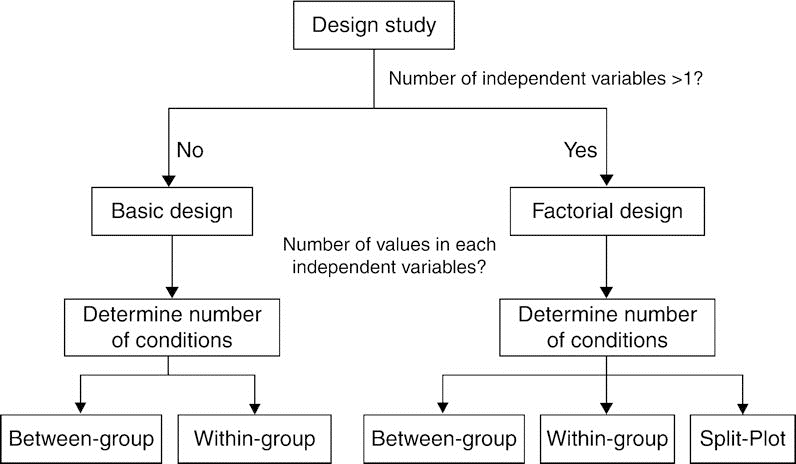
\includegraphics[scale=.5]{Hypothesis1}
\caption{Design study model}
\label{fig:designstudy}
\end{figure}

The difference between the two models is the fundamental test-structure, as seen in figure \ref{fig:designstudy}. In a between-group design, each participant is only exposed to a single experimental condition, meaning in this case he/she would only be playing the vehicle game with one of the controllers, not experiencing them both. In a within-group design each participant will utilize multiple conditions e.g. experiencing two polar opposite ways of controlling a game to establish which is the most user-friendly and convenient.

A within-group approach is usually less time-consuming due to decrease in the number of samples i.e. less test subjects needed to achieve a conclusive result \parencite{Lazar2010}.

Furthermore, Lazar argues that a Between-group construction creates a research setting where it is harder to obtain significant results, because data from different test subjects will have to be analysed under one common denominator. This indicates that a within-group construct would be preferred when choosing the strategic approach. Choosing a within-group construct is, however, not entirely without precautions.
\bigskip

\textit{Since the participants complete the same types of task under multiple conditions, they are very likely to learn from the experience and may get better in completing the tasks.}\parencite{Lazar2010}
\bigskip

This indicates that there is an increased risk of getting biased results, if user-experience is not taken into consideration. If a test subject is introduced to one control-system, and afterwards will try another as to compare the performance he/she may already be familiar with the conditions, and thus a reliable comparison cannot be substantiated. Lazar suggests changing the conditions e.g. altering the sequence of the test randomly per test subject, and furthermore changing the layout e.g. alternative racetrack can plausibly reduce the risk of getting biased samples. 


\subsubsection{Triangulation of data}
Whenever data is collected for any sort of experiment, risks of undermining the data by bias is always present. To prevent evident bias, many different approaches to minimizing the risk of bias can be initiated. 

One, more general, strategy to use, however, is that of data triangulation. The idea behind data triangulation is that by having multiple different data sets (as a result of having multiple tests) from each participant, it is possible to "precisely measure location" \parencite{Lazar2010}; 
in other words -  more accurately measure a tester's response to a product, for example.
\bigskip

An example of how triangulation can be used in practice is first by having the test subject do the experiment, while being observed. Then the test subject is asked about previous experiences (e.g. anecdotes) and their thoughts about similar products. And finally they are asked about future expectations of technology (or whatever subject is being researched).
\bigskip

From these three data sources, an overview of that tester's reaction to technology can be measured - A combination of how the person reacted during the experiment and how they responded to both the questions about past experiences and future expectations. This can give a relatively precise measure of how that person feels about a problem, compared to if they had just been handed a questionnaire, where they, themselves, should rate the product \parencite{Lazar2010}.
\bigskip

The purpose of using triangulation of data, is to minimize the risk of bias, by minimizing the risk of misinterpretation of data - just like it is hard to interpret the direction of a vector in math, from only a single point, it can be hard to interpret the intent of only a single set of data. Whereas multiple data sets (or point, in the context of vectors) will often have a more well defined "heading" (i.e. a user's reaction to a product, for example), thus making it easier to interpret accurately.

That being said, the use of triangulation does still not guarantee bias-free results, as data sources might be diverging, with the data covering different observations. When this happens, the test can still be valid, and triangulation still feasible to some extent, but it is usually not possible to reach a decisive conclusion based on such data alone, which in turn means that further testing might be required if a definitive answer to a test is needed \parencite{Lazar2010}.


\subsubsection{Usability Test}
Testing the product during development is an important aspect of any development process. Usability testing of a prototype involves the user into the testing of the product to make sure that the product is developing in the intended direction, and also determines to which degree the requirements have been proper implemented in terms of functionality. User based testing is usually used to test layouts of user interfaces and other user related aspects of the product.

\noindent Usability testing of a prototype involves \parencite{Lazar2010}:
\begin{itemize}
\item testing prototypes that have only been built on paper (known as paper prototypes);
\item testing prototypes that look complete but have a human behind the scenes responding (known as the “Wizard of Oz” technique);
\item testing working versions of software before it is officially released;
\item testing software that has already been implemented in existing systems. 

\end{itemize}


\subsubsection{Preliminary Test}
The preliminary test is a test prior to the actual test of the implemented product. The test is an examination of the specific method for which the final test is conducted. It will illuminate the different aspects in terms of procedure and results and if the designated procedures are functioning as intended. 

What will be happening, is a preliminary replica of the designated test will be conducted, where instead of having focus on the specific acquired data results, the test is the actual data, from which will be examined to account for the success of the test structure.
 %Moved to evaluation chapter

\subsection{Method: Naïve designs}
The naïve designs are, as the name implies, designs based on assumptions and ideas, instead of actual research or considerations concerning feasibility taken into account. The designs are not meant to be used as a final design, but rather as inspiration source for which areas needs further research, before finalizing the design.

The research which will be considered relevant is the areas of research which proves to be indispensable or in any way plausible to be of relevance to the project. Ultimately, finding the areas of research based on the content of the naïve designs, will help to clarify or in any way specify how to create a product.
\bigskip

The designs start as a brain storm, revolving around ways in which the initial problem statement \textit{could} be answered. The ideas from this brain storm, will then be used to create some design concepts, explaining how a product can be created, how it is intended to work and how it is used to answer the problem. Once the designs are made, thought will go into which elements needs further research, in order to actually make the product described, and to make sure that it \textit{actually} tests, what it is supposed to.
\bigskip

This approach of "Initial Problem Statement -> Naïve Design -> Analysis -> Final Problem Statement" replaces the traditional "Initial Problem Statement -> Investigation -> Final Problem Statement -> Analysis", and the reason this is done, is an attempt at avoiding the risk of getting tunnel vision of a specific way to solve a problem - Instead of focusing on a single way of solving a problem right from the get-go, this approach revolves around having multiple solutions in mind, right up until the point, where the \textit{best} (potentially, at least) solution have been found, through the process of delimitation. 

By having several solutions to the specific problem, the goal is to either choose or combine aspects of the design ideas to conduct a general tender to the solution.

\section{Analysis} \label{sec:analysis}
The purpose of this analysis is to collect the relevant research and data which was deemed necessary during the naïve design phase. This research is going to be used as a basis for a prototype, which should help us answer our problem statement. 

\subsection{Product Comparisons}
As stated by our initial problem, can an ordinary webcam compare to other gaming platforms? It is necessary to figure out which other gaming platforms to compare the webcam with. Since the webcam is a video camera it can be easily be compared with other video game platforms that utilize a video camera. The Xbox Kinect from Microsoft utilizes one RGB-camera and two 3D depth sensors to detect gestures made by the user \parencite{Cong}. The Kinect is popular, having sold roughly 24 million sensors during its current lifespan \parencite{MSByNumbers}, and because it has become such a household name, makes it a suitable platform for comparison.
\bigskip

Another popular brand is the Wii by Nintendo. The Wii was introduced in 2006 and was the first console to have motion control. During its lifespan the Wii has sold near 100 million units worldwide \parencite{NintendoSales}. The Wii also uses a camera but not in the same way as the Microsoft Kinect, instead of using a static VGA camera like the Kinect, the Wii uses an infrared camera positioned within the hand-held controller held by the user to detect the position of the controller in relation to the monitor \parencite{Castaneda2006}. This makes the controller usable as a pointing device. The Wii controller also uses motion sensors to detect the tilting of the controller, which allows the controller to be used as a virtual golf club or tennis racket. The Wii's use of camera technology, makes it suitable for comparison.
\bigskip

The PlayStation Move by Sony was introduced as an add-on to the PlayStation 3 in 2010. The Move uses a video camera in conjunction with motion sensors in a hand-held controller to detect the users position in the 3D space \parencite{Kumar2009}. The move works in many ways as the Nintendo Wii except for the use of camera technology, the Move controller has a visible light on the top of the controller which the camera uses to pinpoint the location of the controller. While the Move is not as popular as the two other products, having sold around 15 million units so far \parencite{Yin-Poole2012}, its use of the camera solution makes it usable for a comparison.

\subsection{State of the art}
To gather knowledge about the process of developing a gaming device using visual computing, the first logical step is to research the "State of the Art", I.e. what have already been done, and how it has been done.

As the problem statement of this report revolves around using a webcam to control a game, it is natural to look at the most dominant solutions on the market, i.e. the Microsoft Xbox 360 Kinect, the PlayStation Move and the Nintendo Wii which will be described the following sections.

The purpose of this research is to gain an understanding of how the team behind the Kinect approached the problem of creating visual computing software, suitable for games, and what they did to solve it, in order to learn from their mistakes and, more importantly, their solutions.

\subsubsection{Development of the Kinect}
\subsubsection*{Kinect}
The Microsoft Xbox 360 Kinect is one of the most successful applications of computer-visual interaction made available to regular consumers of recent years, as proved by the sheer number of sold units during the first 60 days with over 8 million, making it the fastest-selling consumer-electronics device in history \parencite{Knies}.

As the Kinect is probably the most well-known visual computing device for gaming, and it is the device most closely resembling a possible product described by the problem statement, it seems logical to start by researching this.

\subsubsection*{Development:}
At the onset of development, the Xbox development team were using an algorithm that tracked a user's body movement, and used this string of information to 'predict' the movement. Not only were this method a bit unreliable ,it simply couldn't keep up, at times, it was also prone to 'overloading' \parencite{Knies}, even if the algorithm could keep up with the speed of the movement, the tracking would become increasingly more inaccurate over time, and eventually crash, requiring a reset, thus making it unusable for extended game play.

\subsubsection*{Changing the approach:}
The team realized, that they had to change their approach, in order for the application to be suited for video gaming. They figured that as the algorithm crumbled due to it trying to interpret movement from a sequence and therefore trying to predict movement, rather than record it, they needed to change their approach to calculating the movement. \textit{“We couldn’t rely exclusively on context, your history, or your motion in the past. "We realized that we had to look at a single image at a time (...) We had to just look at an image and decide what your body pose was. We knew that this was, in theory, possible, because a person can do this. If you look at a photo, you can draw the position of the joints.”} - Jamie Shotton, 2011.

So instead of trying to predict something as unpredictable as human movement during games, the team figured that the application needed to interpret movement from every frame of a video stream instead - i.e. they needed an algorithm capable of reading a body's position in space from an image, converting said position into data of movement.

Research in this specific field already existed in the computer-vision literature, which made the approach seem promising.

\begin{figure}[h] 
\centering
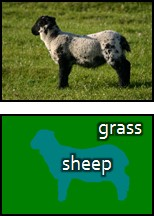
\includegraphics[scale=1]{Sheep1} 
\caption{Sheep-and-grass example.}
\label{fig:Sheep}
\end{figure}
\bigskip

The initial algorithm attempted to match the entire body at once, comparing the image with an extensive database of possible body poses - in essence, the algorithm recorded the body's pose, compared them with the entire library, until it found the best match.

To some extend, the method was functional, but it wasn't going to be efficient enough for the needs of a gaming hardware - As the algorithm checked the entire body at once, it meant that the library had to represent every possible combination of poses, meaning that the library would grow exponentially, causing it to be way too extensive. \parencite{Knies}
The team looked at the existing literature for answers, and found a way to solve the issue:

They had to break up the body into multiple different focus points - i.e. instead of labeling the entire body, they had to identify and label each joint separately.

The way they did this, was to use the "sheep-and-grass" example:
Using an image of a sheep on a grass field, the process isolates the sheep from the grass, automatically labeling the two as sheep and grass, respectively  (fig. \ref{fig:Sheep}).
\bigskip

This principle was used for the Kinect, to label and color parts of a body. Once completed and combined with the gray-scale image from the camera, it was and possible to locate each joint of the body, as the colored parts are defined as being near a joint. By combining the color code of a joint, and the depth information from the gray-scale image, it was possible to estimate the 3D XYZ coordinates of the joint.

\subsubsection*{The Kinect comes to life}
With the object-recognition approach showing promise, the Xbox team started considering how to implement the algorithm on the Xbox 360 hardware, which, at the time, was already three years old. The team needed to figure out a way to implement the tracking algorithm into the existing hardware, taking the ever more demanding games into account.

To solve this, the team used machine learning, and to do this, they needed data.	
\bigskip

\textit{“Mat would feed that motion-capture data into a computer-graphics tool that generated depth images so we’d have something to test on where we knew the right answer. We had a ground-truth answer associated with each image.”} - Fritzgibbon, 2011.
\bigskip

Instead of taking images of real-life people and labeling by hand - a method which is both extremely inefficient and expensive - the team decided to synthesize images, by using computer graphics. After some initial issues with speed or reliability, the team figured out a way to generate the synthesized depth images, which enabled the team to generate millions of images, expanding the training library greatly.

The team then needed to tweak the algorithm to gain greater accuracy, expanding the training library as they went. One problem became apparent, however: it took a very long time to 'train' the program, making the application slow and cumbersome. Using an algorithm dubbed Exemplar ,an algorithm used for object removal and labeling in digital images, \parencite{Cheng2005}, they solved this issue, enabling the application to work fast and accurately enough to run on every single frame of the data-stream of the Kinect depth camera.

Once this was up and running, the team further tweaked the algorithm, enabling them to turn the application to provide a full skeleton, instead of joints, to provide temporal coherence.

By the time the algorithm had been completed, it was capable of processing 30 frames per second, using only 10\% of the Xbox's processing power - thus making it usable for gaming, as less processing power used by controllers (i.e. the Kinect), means more processing power for the actual games.

\subsubsection*{summary:}
Instead of tracking 'nameless' objects in a stream of images, a reasonable alternative is to record, divide, and label each section of an image - i.e. each joint of a body, keeping track of each part of a body individually, instead of trying to record the body as a whole. This saves processing power, and increases reliability and accuracy.
\subsection{Steering Wheel}
Ever since the creation of the electro-mechanical arcade games in the late 1960’ies, the control mechanics has seized to mimic the controls of e.g. real life vehicles \parencite{Herz1997}. With the joystick, the user is given the feeling of flying e.g. an airplane using the rudder stick, and the same goes for the steering wheel, the first which was introduced in 1974 by Atari for Gran Trak 10 \parencite{Kohler2005}. The introduction of the video game console and the personal computer gave competition to the amusement arcades, but opened a separate marked for joysticks, steering wheels and other forms of input devices for home entertainment purposes. 

\begin{figure}[h] 
\centering
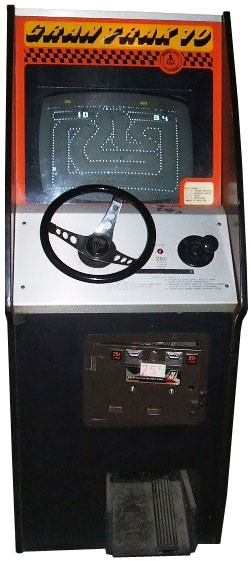
\includegraphics[scale=.33]{Arcade1} 
\caption{A photo of the Atari Gran Trak 10 from 1974, the first arcade vehicle. }
\label{fig:Arcade}
\end{figure}
\bigskip

None of the major motion capture game systems (such as the Wii, Playstation Move, Xbox Kinect) comes with a steering-wheel contraption specifically usable for vehicle-oriented games such as racing games. However, there are several examples of console enhancements that will allow the player to incorporate the steering wheel into their game style, enhancing the game-experience and unlock the natural feeling of controlling, most often, a motorized vehicle.
\bigskip

Where the Wii offers a solution that is compatible with the standard controllers, the X-Box 360 Kinect requires the purchase of an additional controller, which is steering-wheel shaped. Important to note is, that the steering wheel is an independent controller, hence it is does not interact with the Kinect camera. For this particular reason it rather resembles earlier generations of console/PC-steering wheel-controllers, neither which relied on motion tracking by camera.
\bigskip

In between the two is the PlayStation Move Racing Wheel, which is a hybrid of both the Nintendo Wii – and the Kinect steering wheel. Like the Wii, the Move Racing Wheel utilizes the preexisting game-controller, but includes additional functions/relocation of buttons, haptic feedback through vibration, to optimize the game experience.

\subsubsection{Steering wheel functionalities}
\subsubsection*{Introduction}
To account for the functionalities and usage of the controllers, this section covers the remote functionalities of the Wii controller, the Xbox 360 wheel controller and the PlayStation Move wheel controller. This information will make it possible to delimit the functionalities of the games that are developed to that specific console, and therefore controller, since there can only be as much functionality as the controllers support, in terms of buttons and/or motion control as there is available to the specific controller.

\begin{figure}[h] 
\centering
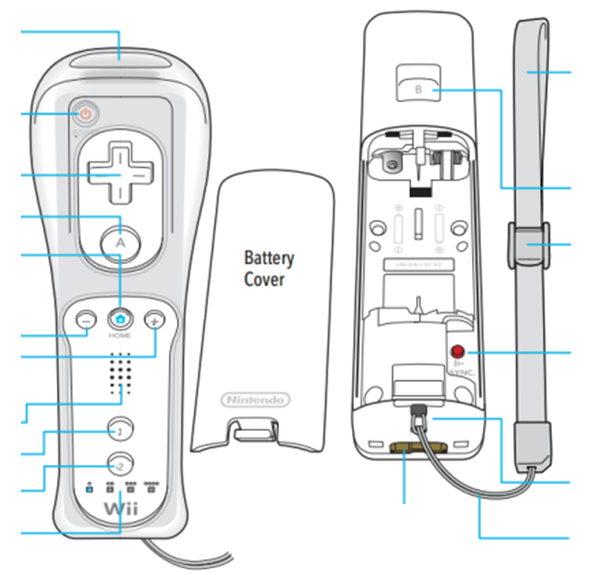
\includegraphics[scale=1]{WiiWheel} 
\caption{Wii Wheel}
\label{fig:Wiimote}
\end{figure}
\bigskip

\subsubsection*{Wii Wheel}
\parencite{Nintendo2013}\newline
As seen on Figure \ref{fig:Wiimote}. the Wii remote functionalities are listed in terms of functionalities and components. The Wii remote is mostly controlled through movement and gestures, so there is only a limited amount of buttons. Being:
\begin{itemize}
\item Control pad (Up, Down, Left, Right)
\item Pointer lens (the method for registering the controller movement)
\item A. \& B. Button
\item Home Button
\item Minus, Plus button
\item 1. \& 2. Button
\end{itemize}
\bigskip

\begin{figure}[h] 
\centering
\caption{Xbox wheel controller description (Danish)}
\label{fig:XboxWheel}
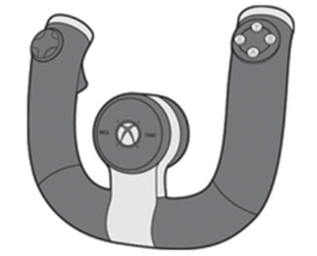
\includegraphics[scale=.75]{XboxWheel} 
\end{figure}
\begin{figure}[h]
\centering
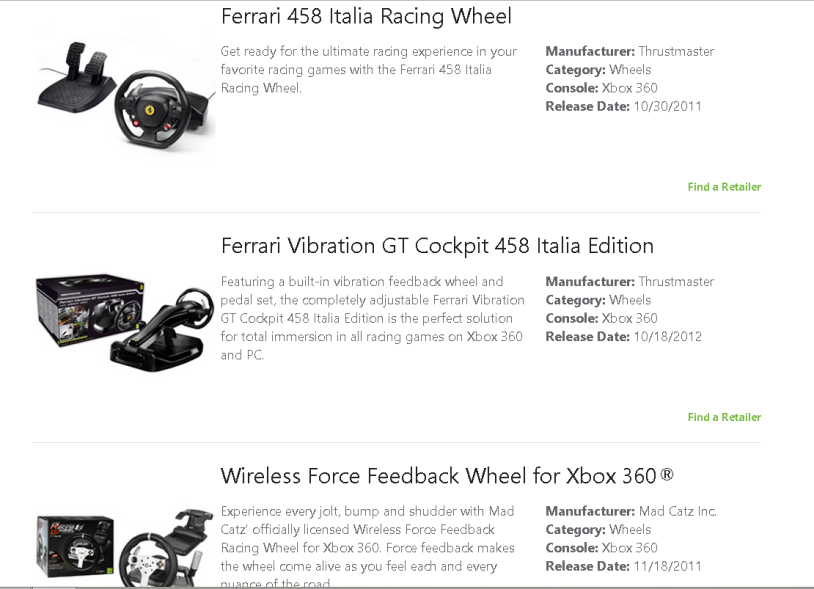
\includegraphics[scale=1]{XboxWheel2}
\caption{Xbox vehicle game controllers}
\label{fig:XboxWheel2}
\end{figure}

\subsubsection*{Xbox 360 wheel controllers}
\parencite{Xbox2013}\newline
As described on figure \ref{fig:XboxWheel}. The Xbox wireless Speed Wheel contains the following features and functionalities:

\begin{itemize}
\item Vibrating feedback
\item Movement tracking sensors
\item Release buttons for acceleration and braking
\item Buttons for game-defined functionalities (Standard Xbox controller functionalities)
	\begin{itemize}
		\item Buttons: A,B,X,Y
		\item Navigation-Button (left, right, up, down)
		\item Guide, start, back ( console control buttons)
	\end{itemize}
\end{itemize}

In addition, there are numerous steering wheel controllers compatible with Xbox that utilizes the same as above mentioned functionalities, but also included features such as floor pedals (throttle, brake, clutch) along with gear controller. See figure \ref{fig:XboxWheel2}. for a list of examples.
\bigskip

\begin{figure}[h]
\centering
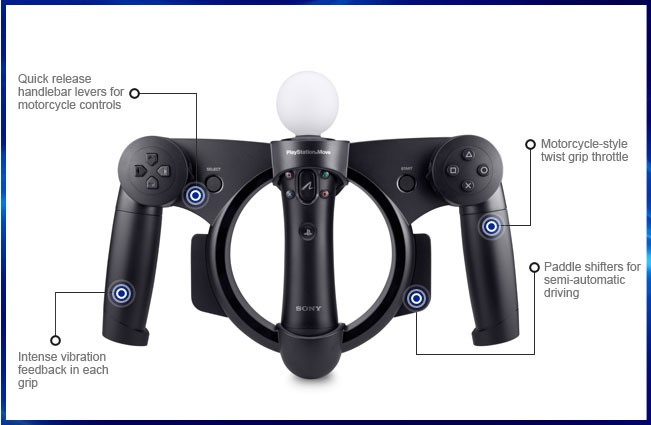
\includegraphics[scale=.5]{MoveWheel}
\caption{PlayStation Move Racing Wheel functionalities}
\label{fig:MoveWheel}
\end{figure}


\subsubsection*{PlayStation Move wheel controllers}
\parencite{Move2013}\newline
As seen on figure \ref{fig:MoveWheel}. The functionalities of the controller are as followed:

\begin{itemize}
\item Vibrating feedback
\item Movement tracking sensors
\item Quick release handlebar levers for motorcycle controls
\item Paddle shifters for semi-automatic driving
\item Buttons for game-defined functionalities (Standard PlayStation controller functionalities)
	\begin{itemize}
	\item Buttons: square, triangle, circle, cross
	\item Navigation-Button (left,right,up,down)
	\item Start \& Select ( console control buttons)
	\end{itemize}
\end{itemize}

\subsubsection*{Summary}
This section describes how the steering wheel controller has been developed to resemble a more realistic and intuitive experience when engaging in vehicle based gameplay. There is also accounted for the design in terms of functionalities of the Wii wheel controller, Xbox 360 wheel controller and PlayStation wheel controllers. This section covers the buttons and other controls of each controller to delimit the plausible amount of functionalities that can be implemented in possible gameplay with each controller.
\subsection{Game controls in various racing games}
\label{gamecontrols}
Within the State Of The Art of the formulated (IPS) area, we have to find out which choices are popular when it comes to deciding how you should be able to control your racing car in the game. This is needed in order to determine which requirements there are to the design of the controller, so that the user will be able to do the same actions in the game, as he/she would be able to perform in the same game played using e.g. Wii or Kinect.

By looking into which games in the racing category are popular on the three gaming platforms Nintendo Wii, Xbox Kinect and PlayStation Move, we can quickly see a difference in the supplies of racing games for the different platforms. It seems that finding a racing game for PlayStation Move is pretty difficult and the most prominent racing game designed for use with PS Move seems to be the game: \textbf{LittleBigPlanet™ Karting} \parencite{Miller2012}. Moving on to the Xbox Kinect; here it also seems that there is only one game standing when looking for the most popular racing game designed for the Kinect without the use of additional controllers, i.e. \textbf{Kinect Joy Ride}\parencite{Davidson2010}. Nintendo Wii, on the other hand, seems to be the most popular gaming platform of the three if you want to play a car racing game. For the Wii there are several different racing games that seem to be popular. Amongst those, we have various versions of \textbf{Need for Speed}, \textbf{TrackMania: Build To Race} and \textbf{Mario Kart Wii}, and \textbf{Sonic \& SEGA All-Stars Racing}, which looks much like Mario Kart in the controls. (This will be explained below) \parencite{Ign2013}.
In order to establish a general rule to follow when you want to create a controller that should be usable with most of the racing games available, a list of the different controls used by the games needs to be made. Making the foundation using the aforementioned 5 games we can assemble the following list:

Consistent for all five games:
\begin{itemize}
\item Steering left and right
\item Acceleration
\item Braking / Reversing
\item Changing camera view (at least for the Wii games - different views from game to game)
\item Display a pause menu
\end{itemize}

Need For Speed (Wii):
\begin{itemize}
\item Nitro (speed boost)
\item Change gear up and down
\end{itemize}

TrackMania (Wii):
\begin{itemize}
\item Braking while accelerating (Drifting)
\end{itemize}

Mario Kart Wii:
\begin{itemize}
\item Choose item
\item Throw items back and forward
\item Perform mid-air tricks
\end{itemize}

LittleBigPlanet™ Karting (Move):
\begin{itemize}
\item Use weapons
\end{itemize}

Kinect Joy Ride (Kinect):
\begin{itemize}
\item Charge and release speed boost
\item Drift to either side
\item Use item
\item Perform mid-air tricks in different directions
\end{itemize}

From this list, it can be seen that there are some general controls that are used through all of these different games. This means that when designing some form of game controller for a car racing game, you should make the user able to perform the five commands listed at the top, as those commands seem to be important, when they are consistent through multiple games. Furthermore, depending on what game we are talking about, there seems to be about 1 – 4 additional controls to be able to play the game fully.


\subsection{Visual Computing}
Visual Computing is computing, which lets the user interact with, and/or control work by manipulating visual images \parencite{Rouse2013}. The visual images can be photographs, 3D-scenes, video sequences or any other visual output for that matter.

It is the core of controlling and manipulating images and is therefore an important aspect to include in the research and find already established solutions to this method.
\bigskip

One example of Visual Computing, which is developed for the PC, is Camspace\copyright. Camspace is a platform for visual computing that, through the use of a standard webcam, detects object and hand gestures and then utilize those to be implemented in games, as a mouse controller etc. \parencite{Camspace2009}

It works as a software platform that is installed on any computer with access to a basic webcam, where options to determine the use dictates how the user interacts with it through human gestures with or without an object.
\bigskip

The program can utilize an object as a controller by presenting a solid object with a uniform color that does not match the environment i.e. the shirt that is worn or the wall behind the player. Also, the room must be well lit for the color recognition to be possible.
\bigskip

Camspace offers games and programs that are specifically designed for the software itself, but does also contain drivers for it to be compatible with pre-existing games, which is developed with other means of control. Although the games are compatible with the software, it is only a limited amount of controls that can be implemented to function with the program.

\begin{table}[h]
\begin{tabular}{| l | l }
Game Title & In-game functionalities\\
\hline \hline
Need for speed underground 2 & Move left/right \& accelerate/break\\
Aquadelic & Left/right \& horizontal\\
Trackmania (\& Nations) & Speed (depth of object) \& left/right\\
LudoRace & Left/right\\
OffRoadArena & Speed(depth of object) \& left/right\\
Flight Model Simulator & N/A\\
Need for speed Carbon & N/A\\
\end{tabular}
\caption{List of vehicle based (driving, sailing, flying) games and the in-game functionalities which is utilized by the Camspace software\parencite{Camspace2009}}
\label{tab:camspace}
\end{table}

\subsubsection*{Summary}
The research indicates that it is possible to create software for computers that utilizes simple webcams for visual computing purposes, such as game control and interaction. It is also possible to modify the use of the program in order to access and control games which is not specifically developed for Camspace itself. Although it is possible, it is only a limited amount of controls that can be imported and utilized via Camspace; (See table \ref{tab:camspace})  such as speed increase/decrease by pulling the designated control object closer or further away, and turn/rotation by rotating the object left or right.
\subsection{Image and video processing}
Because of the initial naive designs, it was determined that image or video processing would be needed to be researched for finding the position of different elements. In this section, methods for detecting objects in an image are therefore being researched. It is necessary to figure out how to detect certain objects in the scene, to use it for controlling things in games or other interactive media.

\subsubsection{Color detection}
A very simple and useful way of detecting objects in a scene, is by using color detection. The drawbacks of this are that it is sometimes necessary to put certain colors on objects that will be used in the scene, in order to make them easier to detect. It is also a good idea to have a background with very few colors, so the colors are easier to seperate. It can limit the colors the user can wear, for example if the camera is set to detect green colours and the user is wearing a green shirt. For example, if an image is searched for green colors, and the user is wearing green, the program will always detect the user. While this might be exactly what the program should do, it would be a benefit to be able to control what to detect, and not just give in to randomness.

To enable color detection, thresholding can be used. Thresholding is isolation of a color or a spectrum of colors. For example, to isolate objects that are very red, the statement r > 200 could be used. This would isolate all colors with a red value greater than 200, turning them white in the output image. Here is a simple example on how to use thresholding, written in pseudo-code. This is assuming the input is an RGB image, and the output is a grayscale image.

\begin{algorithm}[H]
\caption{Color thresholding}
\label{code:threshold}
\begin{algorithmic}
\IF {$ R>R_{min} \; and \; R<R_{max} \; and $\\
	 $ G>G_{min} \; and \; G<G_{max} \; and $\\
	 $ B>B_{min} \; and \; B<B_{max}$\\}
\STATE $g(x,y)=255$
\ELSE
\STATE $g(x,y = 0$
\ENDIF
\end{algorithmic}
\end{algorithm}

In the above example, R, G, and B stand for red, green and blue, and g(x, y) is the output image, where the x and y is the position of the pixel current being processed. For most computers and image acquisition, the RGB color space is used, hence the lack of detail about how to use any other color spaces. In the Gesture Recognition chapter, other color spaces will be discussed, as they make more sense in that situation. The output of the above code would be a binary image. For each pixel in a binary image, it can only have two different values: 0 or 255. This ensures that it is easier for the program to work with, as it only have to compare two values, not 256 values.

Isolating a certain color isn’t enough to actually do something with it though. If one wishes to figure out what position a colored object is at, it is a good idea to find the average center of the detected color. A way of doing this by finding the average position of all the white pixels in the output image. So, for each white pixel, add its x and y position to one variable each, and have another variable that counts how many white pixels there are. Then, divide all the x values added together with the number of pixels, and do the same for all the y values.

The computer now knows the average position of a certain color in the scene. But what if the program should detect more colors? One way of doing this, is to avoid using a binary image for the output, and instead have the output be of many different values and or colors. Each thresholded color then has their own color in the output.

\subsubsection{BLOB analysis} \label{sec:blob}
BLOB stands for \textbf{B}inary \textbf{L}arge \textbf{OB}ject, and in image processing it represents a group of white or black pixels. As mentioned above, it’s possible to detect several colors by having several colors in the output as well. This however means that the program can’t actually separate several objects of the same color. To fix this, a BLOB analysis could be used. To separate each BLOB, a so-called grassfire algorithm 
\footnote{A grassfire algorithm is an algorithm that detects and separates all BLOBs in a scene, by finding a detected pixel, and then labeling all connected pixels as one BLOB (also known as “burning” the pixels).} 
is usually used, with either 4- or 8-connectivity \parencite{Moeslund2012}. 4-connectivity checks the pixels above, below, to the left and to the right of the current pixel, whereas 8-connectivity also checks the pixels diagonally from the current pixel. 8-connectivity is more precise in a sense, since it’s able to detect small diagonal lines unlike 4-connectivity, but it takes more processing power.
\bigskip

The recursive grassfire algorithm, which is usually considered the normal grassfire algorithm, “burns” every white pixel in an image, where the white pixels represent something that has been detected. When the program searches through the image and encounters a white pixel, it’ll run a function containing the grassfire algorithm. This algorithm changes the white pixel to a gray pixel, with a value of 1-254. By doing this, the pixel is “labeled” with a number from 1-254, so the program can find these labeled pixels later. The reason we can’t use numbers below 1, is because that would label the pixel as being black, which the program ignores, and it can’t be labeled above 254, because the program detects it as something white which is has to make computations on, creating an infinite loop.

After labeling, the function will check if there is another white pixel next to the one it just marked. If there is, it’ll label that pixel with the same label as the one before (it will “burn” the pixel), and check if there are any white pixels next to that one. It’s called a recursive function, since it references itself. This continues until the function can’t find any more white pixels connected.
By doing this the program labels each white “island” of pixels, so it is easier to separate them and analyze each BLOB alone.

Note that there is also a sequential grassfire algorithm, which in some cases is more safe to use than the recursive one, since it doesn’t risk running out of memory in the same way as the recursive. The computer only has a limited amount of memory allocated for function calls, and since the recursive function calls itself multiple times, it risks running out of memory if it encounters a very large BLOB, whereas the sequential algorithm doesn’t call itself, and as such doesn’t risk running out of memory. \parencite{Moeslund2012}

\subsubsection{Background Subtraction} \label{sec:BGSub}
The theory behind detecting changes in video is to have a reference image, and subtract that from the recorded image. This effectively removes the background in the image, and leaves only whatever change has been made in the picture. It is also necessary have to perform thresholding, and filter any noise away.

\subsubsection{Other detection methods}
There exist a lot of other ways to detect something in an image or a video feed, for example it might be necessary to detect how much something is rotated, which in turn could require template matching or other methods to find a certain object with a certain pattern.

It can also be useful to be able to track something in a video feed. Arguably some might say that video tracking has already been described in this research, since detecting a certain color for each frame can be interpreted as “tracking” that color \parencite{Moeslund2012}, however that is not necessarily true. In order to actually track something, the program needs to be able to predict where the point it’s trying to track will go to in the next frame. Being as many cameras today run at 24-60 frames per second (fps), an object can’t move too far in an image unless it’s travelling at extremely high speeds.

\subsubsection{Summary}
Color detection is achieved by using thresholding, which isolates certain colors so they can be detected. Color detection is useful if the program only needs to detect one color, or if it needs to detect more than one easily detectable color (for example detection of red, green and blue, in an otherwise white scene).

However if for example a program is required to detect two different players in a two player game, where each player is holding up a red sticker for detection, the program needs to separate these two colors. This is where BLOB detection comes in use, by detecting each BLOB of white pixels, by using a grassfire algorithm. Note that BLOB detection can be used in turn with almost any other detection method, in order to separate objects in the scene.

If the program needs to detect objects that enter a scene, the program can have a reference image of the scene without any objects, and then subtract that image from the video feed. Anything that enters will then stand out. \parencite{Moeslund2012}

\subsection{Gesture Recognition}
The concept is focused on using the user as the controller and letting the movements of the user dictate how the computer should react. In order to accomplish this, knowledge of know how to make the computer understand the user’s intended action is needed. Since the concept will be camera based, the proper tool for reading a user is gesture recognition.
\bigskip

\begin{figure}[h] 
\centering
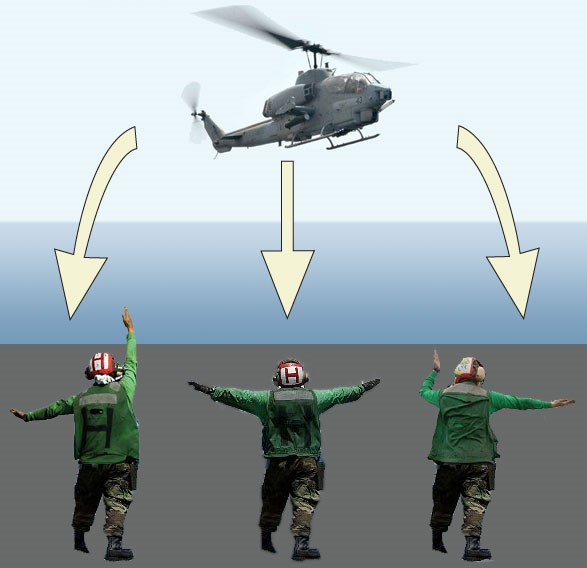
\includegraphics[scale=.33]{Gesture1} 
\caption{Gestures used to communicate instructions to a helicopter.}
\label{fig:Gesture1}
\end{figure}

\subsubsection*{What a gesture is and what they mean in relation to the concept.}
The common dictionary defines a gesture as: \textit{“a movement that communicates a feeling or instruction […]”} and \textit{“to make a movement with your hands or head in order to show or tell someone something […]”}. \parencite{Macmillan2005}
This means that a general gesture is used as a form of speechless communication between two parties used to relay a message or an intent, as seen in Figure \ref{fig:Gesture1} where a movement command is being relayed to a helicopter. Gestures is often used when speech is difficult or impossible.

Because the solution will be based on a camera, then gestures will be the only viable way to communicate an intended action to the computer. Within the scope of the concept, this means that a gesture is a movement, primarily using arms or torso, which communicates an instruction to a computer to be used in an application.
\bigskip

Secondly it is necessary to know how to make a computer understand gestures given to it. For this, image processing is needed.

The first thing that needs to be done to an image of a gesture is to isolate the gesture from the rest of the image. Some methods of doing this includes background subtraction and hue based extraction based on the hue of human skin \parencite{Busaryev}.
\bigskip

Background subtraction \footnote{section: \ref{sec:BGSub}} uses the mean values of a series of images of the same background as a basis for subtracting objects from new images. If a pixel in a new image is different enough from the mean value of the series, then the pixel can be used in a binary image of the objects. The problem with this approach is that variable conditions like lighting and noise can corrupt the results by creating false positives or objects with wrong properties. \parencite{Busaryev}
\bigskip

Another approach is hue based extraction, which converts the image to the HSV (hue, saturation, and value) color space and then uses thresholding to detect human skin in the image. Caucasian skin has a very distinguishable hue values, which make it easier to detect through hue rather than regular RGB. \parencite{Busaryev}
\bigskip

A method of recognizing the gesture is the Local Feature Classifier method \parencite{Busaryev}, which uses the contours of a hand and points along the contour to distinguish for example one shown finger from two and other gestures. With adjustments, this method can be used on bodies and other features.

\subsubsection*{Summary}
In summary a gesture is a movement used to communicate an instruction to a computer to be used in an application. Background subtraction or hue based subtraction, based on the hue of the skin of the user, can be used to extract a gesture from an image. The Local Feature Classifier method can be used to translate the gesture to an application command.
\subsection{User Control Experience}
The focus in this project is to make a controller that is based on the user’s gestures and movements. In order to accomplish that kind of controller a lot of research is required on how the movements has to be executed in order to make it a smooth and positive experience for the user. If this project wants to achieve that feeling it needs research about how the human body communicates by the use of body language. As body language is a huge subject, it has been chosen to only focus on the essentials of the subject and the relevant body parts for the webcam to detect.

In order to create gestures for the webcam to detect there has to be an understanding of what a gesture is. Many have asked this question and according to Adam Kendon an experiment were made with this goal in mind in the year 1978 \parencite{Kendon2004}:
\bigskip

\emph{"What are the features that an action must have for it to be treated as a gesture?"} \parencite{Kendon2004}
\bigskip

This experiment was performed by having twenty people with no psychology or behavioral science background. This background check was made to be sure that it would not have any impact on the test. The people was placed in rooms and told to watch a four minute movie clip without sound made for the experiment. After the movie was done each person was asked to describe what movements they had seen the man in the movie make. The aim was to find out what movements the subjects picked out in their descriptions and to find out what different sorts of movements they identified. After more tests and a lot research the scientists came to a conclusion.
\bigskip

\emph{“Gesture is a label for actions that have the features of manifest deliberate expressiveness. They are those actions or those aspects of another’s actions that, having these features, tend to be directly perceived as being under the guidance of the observed person’s voluntary control and being done for the purposes of expression rather than in the service of some practical aim.”} \parencite{Kendon2004}
\bigskip

As recording to the research, gestures have a huge impact on the listeners. Even though webcams do not have any ears these theories can still be of use for us. As Susan Goldin-Meadow writes in her book \parencite{Meadow2005} people still use gestures even though they are not communicating with another person. This could be you at home practicing a speech or simple just talking to yourself. You talk but even if you are the only one in the room you would still perform your gestures, as you were trying to explain something to another person.

Now that it is known what a gesture is, the research can continue on which gestures needs to be implemented. A few common gestures have been found that are being used in the daily lives that could be useable for the webcam to detect \parencite{Businessballs}.
\bigskip

Common gestures:

Hands:
\begin{itemize}
\item Thumb up - positive approval, agreement, all well
\item Thumb down - disapproval, failure
\item Index finger and thumb touching at tips - satisfaction
\end{itemize}

Head:
\begin{itemize}
\item Head nodding - agreement
\item Head shaking - disagreement
\end{itemize}
\bigskip

A last thing of mention is that people has a personal space also called Proxemics with five different comfort zones. close intimate, intimate, personal, social-consultative and public. All of these zones define how comfortable the person is with another person standing around them. So this is something that should be kept in mind when creating the controller. If the aim will be for the Social-consultative and Public zone. It is then important according to Edward Twitchell Hall that we place cameras and other players at least 1.2 meters away from the player in order for the person to feel comfortable between themselves and others \parencite{Businessballs}.

So what can be concluded from this research is that in order to make a good controller that is based on the user’s gestures and movements. A test has to be made in order to show how people want to handle the different movements and actions that the webcam will observe. With the information received from the initial tests it is then possible to create a pattern that fits the majority of volunteers used for initial testing. After that it should be possible to implement the right movements and gestures for the controller and then give the right instructions for our movements at the final test.  This process should make it a smooth and positive experience to use the controller created for the project.


\subsection{Analysis summary}
From the analysis, some key elements were found, in regards to the initial problem statement, and how to create a solution for the problem.

The first point that becomes apparent is that while the initial problem statement is technically solved by using Camspace, it also proves to be insufficient for the desired use - As the controls are limited to movement, and not special actions. This is further emphasized as a problem, when looking at the fact, that none of the researched racing games make do with simply movement - they all have one or more additional features, which are essential for the game play.

Another important section of knowledge gained from the analysis, is the different ways to create the program - The analysis shows different methods of doing it, and gives arguments for how each method could be used, which will help deciding, when the product is going to be designed.
From the analysis, the initial problem statement can be modified, and turned into a final problem statement, with which to continue work on the project.

\subsection{Final Problem Statement}
How can we create a controller that utilizes visual computing within the limitations of a webcam to create a vehicle controller with the following functionalities?
\begin{itemize}
\item Left / Right
\item Acceleration
\item Brake / Reverse
\item Gear shift
\item (extra): Action button
\end{itemize}
Additionally, how does the constructed controller compare to a regular controlled vehicle game in terms of functionality and playability.
\section{List of Requirements}
\label{LOR}

\textit{The content of the list of requirements is to be seen as parameters for the product design. The arguments have been refined in the analysis-chapter, and have ultimately led to these requirements, that will help construction of the final product. Hence it is to be considered a blueprint from which numerous variations of designs can be crafted.}
\bigskip

General requirements:
\begin{itemize}
\item The controller must be for controlling vehicle games.
\item The controller must utilize visual computing within the limitations of a webcam.
\item The controller must be comparable to pre-existing controllers in terms of functionality.
\end{itemize}
Hardware requirements:
\begin{itemize}
\item Standard webcam
\item Computer
\item No additional technology required for the sake of control of the vehicle game.
\end{itemize}
Software requirements:
\begin{itemize}
\item The controller software must be compatible with preexisting vehicle games.
\end{itemize}
Controller functionalities:
\begin{itemize}
\item Steering left and right
\item Acceleration
\item Braking and/or driving reverse
\item Gear shift
\item (Extra) action button for utilities 
\end{itemize}
\section{Design}
Introduction missing.

\subsection{Design one}
\label{design1}
This design revolves around the user being able to customize almost everything. The design therefore aims to be very flexible, and to accommodate almost every situation. The design of this system is structured with the following overview:

\begin{itemize}
\item user created wheel with attached stickers for camera registration and detection which will be utilized to accommodate several controller functionalities.
\item Additional gestures, not utilizing the wheel, which will accommodate controller functionalities.
\item Several possibilities to alter the specified gestures and functionalities to the users preferences. 
\end{itemize}


\subsubsection*{Description}
The user in this design will be given 3 or more stickers of different colours. See figure \ref{fig:wheel}. In this example, a red, green and a blue sticker are used, but since the design is so customizable, the user should be given the ability to choose colours him/herself. The user can also make the stickers themselves, in which case the design is completely free for the user.


\begin{figure}[!htbp]
\centering
\subfigure[example sticker configuration.]{\label{fig:design11}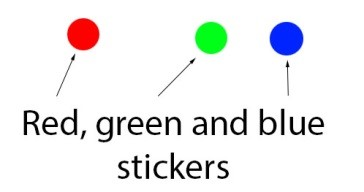
\includegraphics[scale=1]{Design11}}
\subfigure[Object for steering with stickers on.]{\label{fig:design12}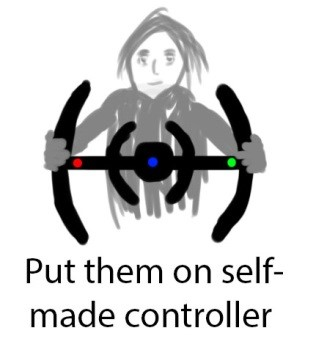
\includegraphics[scale=1]{Design12}}
\caption{Sticker configuration.}\label{fig:wheel}
\end{figure}

The user then places these stickers on some object he/she would like to use as a mean of controlling a vehicle inside a game. In this example, the stickers are placed on a steering wheel, which could be cut out from cardboard.

\begin{figure}[!htbp]
\centering
\subfigure[example of what the menu for steering could look like.]{\label{fig:design14}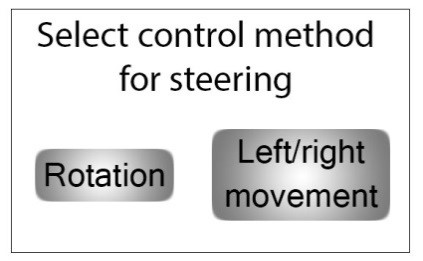
\includegraphics[scale=1]{Design14}}
\subfigure[example of what the menu for acceleration could look like.]{\label{fig:design13}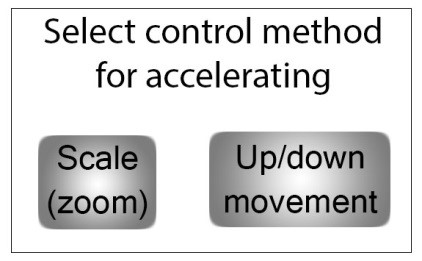
\includegraphics[scale=1]{Design13}}
\caption{Menu examples.}\label{fig:select}
\end{figure}

The user then picks how he/she would like to use the object for steering. Only two options are listed in this example, but more could be added, including ways of customizing the control method e.g. for example, choosing how much you should be able to rotate the controller before reaching the maximum turning speed. See figure \ref{fig:select}.
\bigskip

Customization is also allowed for acceleration in which case the user can choose between moving the controller closer or further away from the camera, moving the controller up and down, or moving one hand up or down separately from the steering wheel. 
The acceleration itself would simply change between max acceleration and no acceleration at all, or acceleration, no acceleration, and breaking, for simplicity. A separate sticker placed inside one’s hand can be used for braking, if it is needed to brake and use the speeder at the same time.
\bigskip

Gear shifting can be set up by being the “opposite” of controlling the speed. So if the user chooses to use up/down movement of the controller for speed, the user can use his/her free hand to separately control the gear shift. If the user holds their hand, with stickers attached, high, it would change the gear up, if the user holds it low, change the gear down, and if it’s in the center area, do not change gear. See figure \ref{fig:design15} for example of rotation and gear shift.

\begin{figure}[!htbp]
\centering
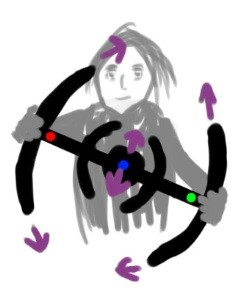
\includegraphics[scale=1]{Design15}
\caption{Controller in use.}
\label{fig:design15}
\end{figure}

To implement and extra action such as using power-ups or something similar, the opposite
of the steering control method could be used. If the user is using rotation for steering,
left/right movement could be used for extra action functionalities, and vice versa if the user
chose left/right movement for steering. After everything is set up, the user now has his/her own custom-made controller, unlike any other. He/she can use it to control vehicles inside game, only needing a webcam to pick up the colours, and a computer.
\bigskip

As a prototype using this design, the control methods that are to be implemented are listed below in categories of what actions the methods are used for. As mentioned the user will choose between one of the methods listed for each action. One method can be listed for two different actions, but if the user chooses one method for one action he/she can not choose it again for another action. The list is as follows:

\begin{itemize}
	\item Steering the car:
	\begin{itemize}
		\item Rotation – Tracking rotation movement of stickers placed on the controller.
		\item Left/right movement – Tracking stickers on the controller moving horizontally.
	\end{itemize}
	
	\item Acceleration \& braking:
	\begin{itemize}
		\item Up/down movement – Tracking vertical movement of the stickers.
		\item Forward/backward movement.
		\begin{itemize}
			\item Tracking change in distance between stickers on the controller.
			\item Tracking change in size of one sticker (or multiple).
		\end{itemize}
	\end{itemize}
	
	\item Gear shifting:
	\begin{itemize}
		\item Up/down movement – As above.
		\item Forward/backward movement – As above.
		\item Hand gesture, up/down movement – Tracking vertical movement of a sticker on a hand. Here the user must release the controller with the one hand.
	\end{itemize}
	
	\item Extra action:
	\begin{itemize}
		\item Rotation – As above.
		\item Left/right movement – As above
	\end{itemize}
\end{itemize}
\bigskip

This design will output the users commands as simulated presses to the keyboard. 
Because the keyboard mappings differ from game to game, the individual keys that should be simulated by the software will be provided to the software by a profile.
The profile will contain a mapping of the command types to the keys that should be simulated. 
The software should have no interaction with the game other than the simulated keyboard presses.

\subsubsection*{Compared to the FPS and List of Requirements}
The FPS is focused on creating a cheap alternative to already existing vehicle controllers. This design not only creates a solution that needs nothing else than a standard laptop, it also lets the user specify and control almost every aspect of controlling, and lets them create their own controller. It is not even necessary to make a controller; the user can paint their hands and use them instead if they want.

Compared to the list of requirements, this design fulfills everything but the ability to brake while accelerating, nor gear shifting. In the example explained, it also does not fulfil the ability for extra action buttons. However the design can be made more complete to allow such control methods, without the need of additional purchases, such as buttons, by adding customization options to the user.


\pagebreak[2]
\subsubsection*{Pros and Cons}
Pros:
\begin{itemize}
\item It is free of cost, provided the user has a computer and webcam.
\item Potentially adds an infinite number of customization options.
\item It is not limited to a single game.
\end{itemize}
Cons:
\begin{itemize}
\item The amount of setting-combinations could potentially be complicated for the user.
\item It could, be potentially, hard to make.
\end{itemize}

\subsubsection*{Software specifications}
In order to conduct tracking, colour tracking can be used as described earlier. This method would likely be the simplest and easiest way to utilize tracking through a standard web cam. However, there is several limitations to colour tracking such as colour usage which might be worn by the user and therefore limits the usage. Additionally, lighting and other room conditions can alter the usability of colour recognition.

Potentially, pattern recognition or template matching can be an alternative to colour recognition, diminishing the specified complications. In this case, the surrounding environment is not compromised in terms of colour or light.


\subsection{Design two}
Compared to several of the vehicle game controllers available this design steps away from controlling the vehicle using a steering-wheel-like controller. In this design, the user grabs hold of two blocks and moves these around on a flat surface (e.g. a table), thus controlling the behaviour of the car.

\subsubsection*{Description}

\begin{figure}[h]
\centering
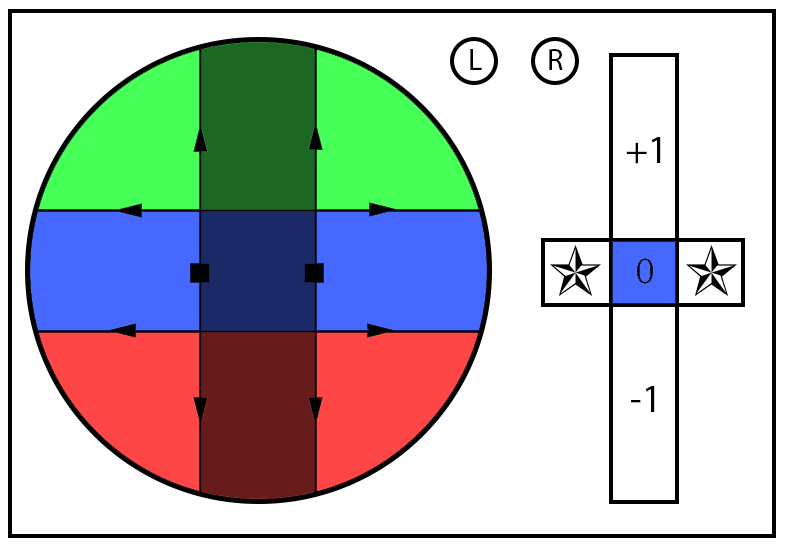
\includegraphics[scale=.75]{Design21}
\caption{Playing area.}
\label{fig:design21}
\end{figure}

What the user need in order to be able to control the car using this design is two blocks of different colours that can be held without covering the top of the block. Next, the user needs a webcam, which will be placed over the area in which the user is moving the blocks around in looking down (to see the top face of the blocks). Ideally the user would also have a piece of paper (preferably A3 or larger) with the “playing area” drawn onto it.
\bigskip

The “playing area” is illustrated on figure \ref{fig:design21}, where on the left side a circle is drawn. The user will move one of the blocks around in this circle and the car will accelerate when the block is in the green areas, decelerate when in the red areas and neutral when in the blue areas. By moving the block to the left or right (i.e. moving the block inside one of the bright-coloured areas), the car will turn accordingly while still accelerating, decelerating or none of those.

The other block used in this controller, is used to change the gear up and down and to activate additional features (currently this design supports two additional features). The shape on the left side of figure \ref{fig:design21} is where this other block is used. When the user is not changing gear or activating another feature, the block is to be placed inside the blue tile containing the number “0”. If the user will move the block up or down to change gear up or down accordingly (into the tiles tagged “+1” and “-1”). To activate on of the additional features, the user will move the block either left or right from the blue tile and into the tiles with the stars, which will then activate the feature set to the respective tile.

In the top of figure \ref{fig:design21} there are two circles marked “L” and “R”. Each of the two blocks will be placed in one of the two circles before the controller will be active. This means that the controller has to determine the block that is used to turn and accelerate/decelerate the car, which will be placed in “L”, while the block placed in “R” will be used to change gear and activate additional features.

Though the user does not need the playing area to be drawn on something in order to use the controller, it would be easier for the user to keep track of what control he/she is activating, when the tiles are illustrated beneath the blocks. However, the colours used in figure \ref{fig:design21} are not mandatory, but simply used in order to ease the description.

\subsubsection*{How does this design fulfil the design requirements? (IGNORE TEMPORARILY)}

\subsubsection*{Pros and cons}
Pros:
\begin{itemize}
\item The controller is very different from other controllers which might arouse curiosity
\item Only a computer and a webcam needs to be bought, other materials can be homemade
\item Is usable for several racing games (or alike)
\item Can be expanded to support several additional features (e.g. up/down gear-shift could be replaced) or additional tiles could be added.
\end{itemize}
Cons:
\begin{itemize}
\item Could be difficult to place the blocks on the tiles precisely while maintaining the focus in the game.
\item With the current setup, the user needs the computer and webcam to be separated, thus eliminating the use of a laptop with its webcam.
\end{itemize}

\subsubsection*{Image Processing.. how?}
In order to detect how the user is moving around the blocks, colour recognition would be an easy way to distinguish between the two blocks. The two blocks could be separated as two BLOBs and according to each BLOB’s position in the frame, captured by the webcam, relative to the tiles in the playing area, the user’s intention could be registered. This however, would require the blocks to be of easily distinguishable colours that does not blend-in with each other or the colours in the background.
\subsection{Design three}
\subsubsection*{Description}
The idea behind this design is to come as close to preexisting methods of controlling a vehicle game without using an actual controller. This should be done by only utilizing single standard webcam and color recognition for tracking controls and functionalities. The user is required to make/or obtain any desired material that the user wishes to use as controller material e.g. cardboard, piece of paper etc. (theoretically any object should be viable). Thereafter create the desired shape and size representing the steering wheel. 
Additionally image BLOBS (See figure \ref{sec:blob} in report for description) will be used to control the game. 
\begin{figure}[h]
\centering
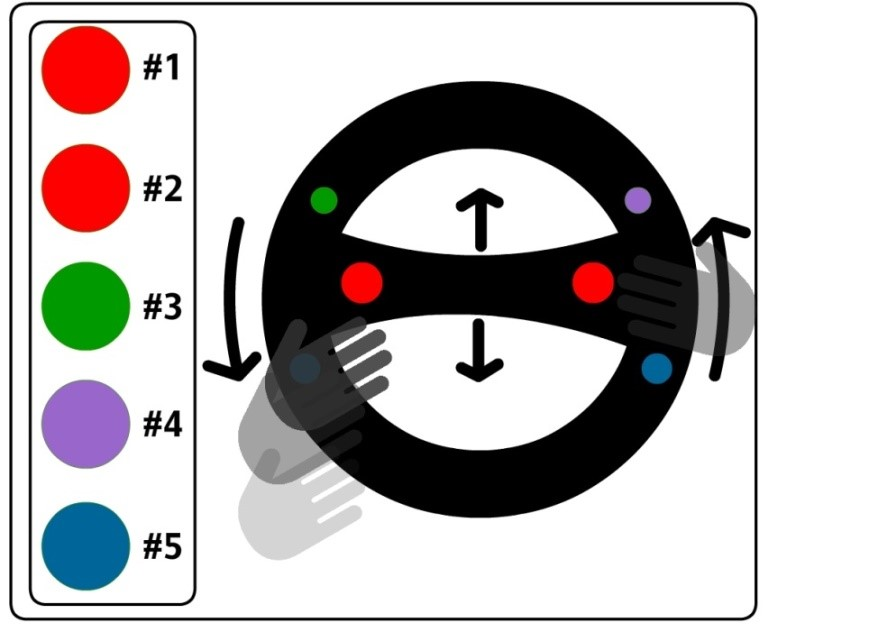
\includegraphics[scale=1]{Design31}
\caption{Controller: Blob and movement description}
\label{fig:design31}
\end{figure}

As seen on figure \ref{fig:design31}, BLOB \#1 \& \#2 is for implementing rotation and depth for controlling the vehicle forward, backward, and breaking. These BLOBS must be visible and placed adjacent and horizontal to one another. This is to ensure that the tracking of rotation and depth is possible.

Additionally, the BLOBS \#3, \#4 and \#5 will be visible, but perform no functionality before the user blocks the BLOB and thereby activating the desired function/ability of the designated BLOB. By utilizing this method, the procedure of pressing a button is reconstructed and therefore imitates a real controller.
\bigskip

This design will output the users commands as simulated presses to the keyboard. 
Because the keyboard mappings differ from game to game, the individual keys that should be simulated by the software will be provided to the software by a profile.
The profile will contain a mapping of the command types to the keys that should be simulated. 
The software should have no interaction with the game other than the simulated keyboard presses.

\subsubsection*{Functionality description} \label{Dfunc}

\begin{figure}[h]
\centering
\caption{BLOB blocking illustration}
\label{fig:design32}
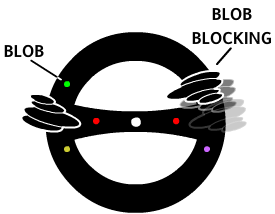
\includegraphics[scale=.75]{Design32}
\end{figure}

\begin{figure}[h]
\centering
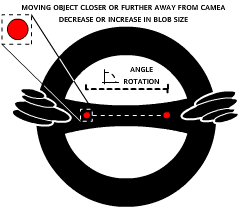
\includegraphics[scale=.75]{Design33}
\caption{Rotation \& forward/Backward}
\label{fig:design33}
\end{figure}

By implementing functionalities that is activated by blocking specific BLOBs, it is possible to add numerous functionalities by just adding more BLOBs to the controller. 

By designing the controls in this specific manner, the activation would, theoretically, be easy accessible. This will make it possible for the user to quickly activate certain functionalities or make a specific row of operations, which with movement could be somewhat problematic to perform simultaneously. 

One negative aspect of the technique is that it is likely that depending on the positioning of the BLOBs, several functionalities might be accidentally activated. Furthermore, since the controller will have to be positioned towards the webcam in order to track the BLOBs, the user will not be able to see the designated “button” that is present on the controller, and will therefore have to remember the placement of them and will only get feedback from the performed action, in game, if the action is registered in the first place.


\subsubsection*{Compared to the List Of Requirements and Final Problem Statement.}
As described in the Final Problem Statement (Section: \ref{sec:fps}, page \pageref{sec:fps}), the following functionalities are implemented:

\begin{itemize}
\item Steering left and right (See fig. \ref{fig:design31})
	\begin{itemize}
	\item o	Two BLOBs placed horizontally adjacent to each other will make it possible to detect rotation and therefore making it possible to steer a vehicle.
	\end{itemize}
	
\item Moving forward \& backward/breaking (See fig. \ref{fig:design33})
	\begin{itemize}
	\item By moving the object closer or further away, we are able to detect the movement and therefore track the vehicle moving forward, backward or breaking.By moving the object closer or further away, we are able to detect the movement and therefore track the vehicle moving forward, backward or breaking.
	\end{itemize}
	
\item Shift gears
	\begin{itemize}
	\item By implementing two BLOBs with separate colors, when the specific BLOB is blocked and therefore not visible, the implemented functionality of gear shift is activated, up or down depending on the implemented functions.
	\end{itemize}
	
\item Utility Button(s)
	\begin{itemize}
	\item For each game, there are several functionalities which are specific for that game. Therefore a BLOB, with the same procedure as the BLOBs for shifting gears will be implemented.  That will have functionalities which will be defined by the specific vehicle game that is being played. This can be extra utilities such as power boost, attack, etc.
	\end{itemize}
\end{itemize}

\subsubsection*{Pros and cons}
Pros:
\begin{itemize}
\item The user is able to create a controller with a shape and size, which is suitable for the individual’s preferences.
\item The required BLOBs except the two red BLOBs that is used for rotation and depth, can be placed anywhere on the assembled controller which is suitable for the individual preferences of the player. 
\item Since activation of functionalities only requires that a certain BLOB is blocked, possibly several functions can be activated simultaneously or rapidly after one another without much delay or effort based on the positioning of the BLOBs.
\item It is possible to implement a large number of additional functionalities.
\end{itemize}
Cons:
\begin{itemize}
\item As mentioned in Functionality description (\ref{Dfunc}); By implementing several features and functionalities it is possible to cover several BLOBS by accident and therefore activate undesired functionalities.
\end{itemize}

\subsection{Design delimitation}

To delimit the three designs, to the actual design that will be implemented, each design will be compared to the list of requirements. Here the design ideas will be evaluated in terms of how well each specific design fulfil the requirements and therefore might answer as a possible solution to answer to the final problem statement. See section \ref{LOR} for the list of requirements

\begin{itemize}
\item The controller must be for controlling vehicle games.\newline
Each design is specifically developed with vehicle games in mind. Therefore no specific features of any of the ideas is relevant in terms of this specific requirement.

\item The controller must utilize visual computing within the limitations of a webcam.\newline
Each design idea is based on a standard webcam. No design idea has any special requirements beyond those defined in section \ref{webcam}. 

\item The controller must be comparable to pre-existing controllers in terms of functionality.\newline
All of the design ideas are developed based on the commonly utilized controls as researched in \ref{gamecontrols}. Therefore this requirement is fulfilled by each of the three design ideas.

\item The solution must require a standard webcam.\newline
All three design ideas is based on utilizing a standard webcam, except design 2 which requires setting up the webcam in a specific way.

\item The solution must require a computer to run the software.\newline
All three design ideas is based on utilizing a computer to run the software.

\item The standard webcam does not have to be embedded in the computer. Therefore computer type is irrelevant.\newline
None of the design ideas specify additional requirements to the computer that should be used, therefore this requirement is fulfilled by all three design ideas.

\item No additional hardware required for the sake of control of the vehicle game.\newline
The design ideas specifies that computer hardware is required. Additional items are accessories which must be utilized to control the software on said hardware, and does therefore not count towards additional hardware. This is the case for all three design ideas. Note however that some might consider webcams as being additional hardware.

\item The controller software must be compatible with a pre-existing vehicle game which supports
the game functionalities as described in Controller functionalities.\newline
Each design idea simulates keyboard buttons as output to each game. This means that the controller should be compatible with vehicle games that might deviate in control scheme.

\item The output of the software should mimic input to conventional input methods like keyboard
presses or mouse movements.\newline
The design ideas simulates keyboard presses to send commands to the game. 

\item The controller software must track either colors, patterns or both.\newline
With each design, the method of controlling the tracking method is specified as color detection. As described in fiducials (section: \ref{sec:detect}) there is specific pros and cons for each method of tracing, and both can basically be implemented in each of the three designs and have the same specified functionalities as the other.

\item Controller functionalities.\newline
All three design ideas are developed with the specific controller functionalities in mind, and does therefore include all of them. The controller functionalities being steering left and right, Acceleration and braking/driving reverse, gear shift and an optional action button for utilities.

\end{itemize}

As described in the previous delimitation, all the design ideas satisfy the list of requirements to the same degree, therefore each design could be used to answer the final problem statement.
As per requirement given the project structure, it is a needed delimitation that a single design concept is chosen to take into further development. Based on the above mentioned section it can be established that all designs are equally capable of containing the requirements and ultimately answer the final problem statement. There are, however, both strengths and weaknesses in the design, and these have been discussed internally. The following section will account for the choice of Design idea 1. See section \ref{design1}.	

Design idea 2 (section \ref{design2}) differs from the other two design concepts due to the requirement of an external webcam and a mean to attach it above the gaming surface. This might ultimately go against the project concept that states that the artifact is required to be easily accessible and usable by most. Therefore it is estimated that more integrated webcams are predominantly accessible by most of the target group. For this reason the design idea 2 has been downsized. Design idea 3, see section \ref{design3} for description, utilizes the integrated webcam; however this design concept does not include gestures, which mean that BLOBs will have to be used instead to cover the requirement of functionality that must be comparable to SOTA-controllers. The BLOBs will have to be situated on the opposite site of the race-wheel, which ultimately can make it harder for the user to see where he/she is placing the fingers to block the BLOBs. Using BLOBs as buttons is risky, since electronic buttons will always have an advantage in this regard. Additionally the specified numbers of functionalities might cause plausible difficulties when several BLOBs are placed upon the controller. Thus making it likely to accidentally activate several functions, or making it generally difficult to manage said controller functionalities. Currently, the only disadvantages of design idea 1 is that it requires more thorough image processing to work, and might be more time consuming, and also more complicated for the user to learn, since an implementation of several functionalities will have to be implemented. The final decision was ultimately between design idea 1 and 3, and given the comparison between the cons, it was established that design idea 1 will potentially render the most positive result, and make room for customization of the design-content if certain approaches are found to be an impasse. 

\section{Implementation} \label{sec:implementation}
On the basis of the chosen design, from the design section, a prototype will be built, and later used for testing.
Throughout this section, there will be a presentation and discussion of how this prototype has been implemented. 
The implementation consists of two parts: first a software part, where the programming of the application will be described, and second, a description of the physical artefacts that will be used for testing.

\subsection{Physical artefacts}
As explained in the chosen design, the idea with the physical artefact used as a part of the game controller, is that the user should be able to fully customize it him-/herself. 
In order to create a prototype usable for testing, a simple wheel-like controller has been created used to control the acceleration, braking/reversing, camera view and steering of the car. 
Additionally, to shift gear up and down, a yellow sponge was used and managed with the right hand. 
In figure \ref{fig:imp1} a picture of both the sponge and the wheel-like controller is shown. 
The sponge is used as the yellow color is fairly easy to distinguish from other colors. 
The wheel controller in the right side of the figure is made of a piece of cardboard with an attached A4-sized piece of paper, on which is printed three colors. 
This wheel has the two main colors, red and blue, which are used as fixation points to determine the right and the left side of wheel. 
These two creations, the sponge and the wheel, are examples of how a user could choose to design his/her own controller.
\bigskip

\begin{figure}[!htbp]
\centering
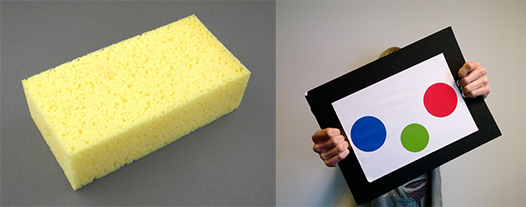
\includegraphics[width=4in]{Imp1}
\caption{The physical part of the racing game controller. (left) A sponge is used to change gear and (right) a wheel-like controller is used to steer, accelerate/decelerate the car and change camera view.} 
\label{fig:imp1}
\end{figure}

The way the wheel controller is used, is by rotating it, like a typical vehicle wheel, in order to turn the car in the game. 
Also, the wheel can be moved towards and away from the camera to accelerate and decelerate accordingly, while moving the wheel to either the left or the right will activate an extra function in the game, which here has been chosen to be changing the camera view. 
The sponge, however, is used to shift up and down in gear by raising or lowering it with the right hand accordingly. 
This means, that in order to change gear, the user will have to let go of the wheel with the right hand to raise/lower the sponge in front of the webcam, which again is an example of how a user can freely choose how he/she wants to manage those three required fixation points.

\subsection{Development of the software application}
The main part of this prototype consists of a piece of software developed for registering input from the user and deliver this information to a racing game, which will give the user the ability to control a car in a game. 
The software that will be described in this chapter is based on the C++ programming language. 
As the idea of registering input from the user is based on visual computing, the open source C++ toolkit “openFrameworks” has been used, as this toolkit works very well with visual computing.
To describe the software developed for this prototype, first a walkthrough of the flow of the application will be presented followed by a description of specific parts of the code.

\subsubsection{Flow of the application}
To be able to use the controller the user has to start up the software on a computer with a webcam connected to it. 
In figure \ref{fig:imp2}, a flowchart of what happens when the user performs certain actions in the user interface is presented. 
Starting from the top left of the figure, a dot represents the user starting the program, which immediately leads the program to the main menu.
\bigskip

\begin{figure}[!htbp]
\centering
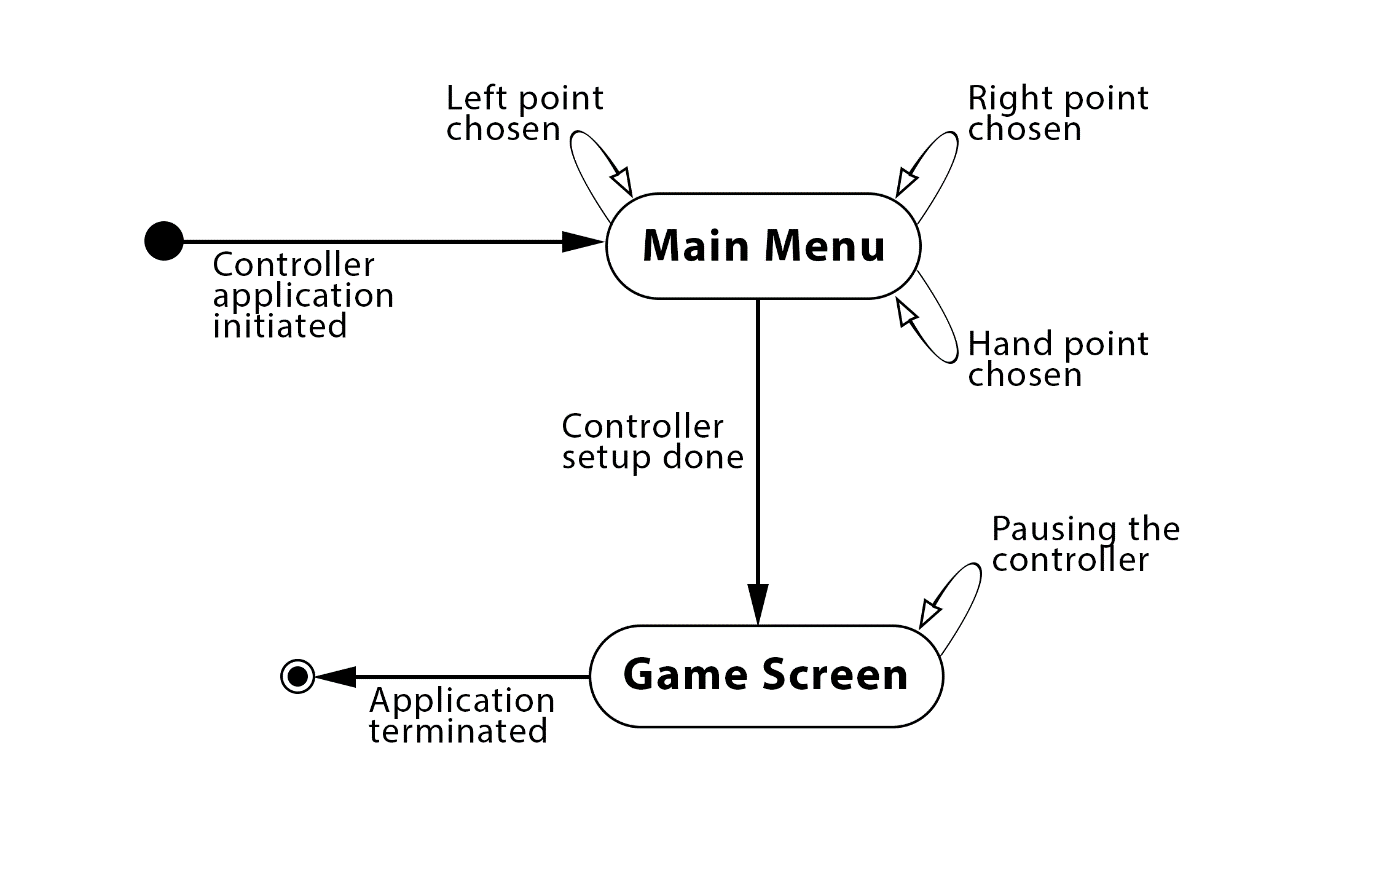
\includegraphics[width=4in]{Imp2}
\caption{State chart.} 
\label{fig:imp2}
\end{figure}

In the main menu, the user is asked to give some information about which colors, in the image captured by the webcam, are used as the left and right point of the wheel-part of the controller. 
These two colors are chosen by marking the area in the image, in which each of the colors are represented. 
In figure \ref{fig:imp3} an example of choosing the colors can be seen. 
First, the left point (the red color on the controller) has been chosen, by clicking on the little box to the left of the text saying “Add left point”.
Hereafter, the user has to click and drag on the image to the left in the figure around a part of the red mark on the controller. 
The program then finds all the red-colored pixels in the left image and represents them in the right image as pure red pixels. 
After choosing the left point, the right point can be chosen, which is the ongoing action in the figure. 
The last point, “hand point”, is the color that should represent the gear-shifting controller, described as the yellow sponge earlier.
\bigskip

\begin{figure}[!htbp]
\centering
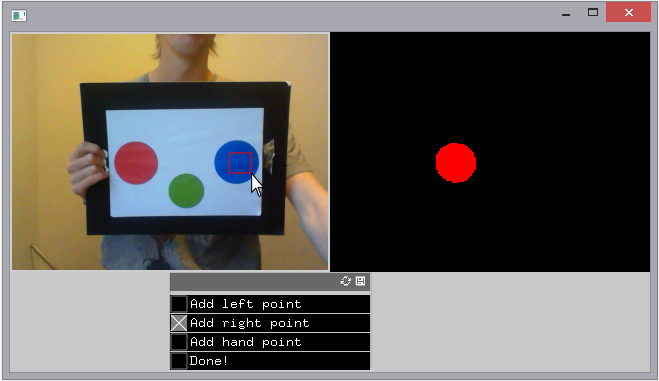
\includegraphics[width=4in]{Imp3}
\caption{Window showing selection of color tracking.} 
\label{fig:imp3}
\end{figure}

Back in the flowchart in figure \ref{fig:imp2}, the arrows going out and back into the main menu, illustrates that, when the user selects a color to use as one of the points, it is registered, but the main menu keeps open. 
When the user clicks “Done!” (see figure \ref{fig:imp3}), the setup of the controller points is finished, which leads the program to the game screen. 
The game screen takes care of registering what the user does in order to tell the car in the game how to behave. 
An example of how the game screen looks when the program is running can be found in figure \ref{fig:imp4}. 
Here, each of the points are shown as the red, green and blue circles on the left image, while the yellow circle is the centre point between the right and left point of the wheel controller. When the yellow circle is moved either to the left or the right of the magenta box, the camera view in the game will be changed. 
A more thoroughly description of the game screen, including how the other game actions are activated, will be presented in the following chapter (\ref{sec:codedesc} Code description).
\bigskip

\begin{figure}[!htbp]
\centering
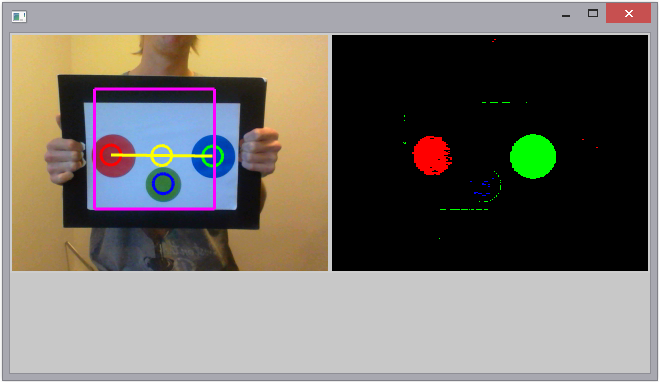
\includegraphics[width=4in]{Imp4}
\caption{Window showing active tracking.} 
\label{fig:imp4}
\end{figure}

When the game screen is shown, it is possible to put it on pause, if the user for some reason would have to temporarily turn off the controller. 
In the flowchart on figure \ref{fig:imp2}, this is illustrated as the arrow going out from and back into the game screen. 
When the user finally wants to turn off the controller, the application can be terminated by either pressing the escape button (esc) or clicking the X in the top right of the window, which, in the flowchart, is represented as the arrow pointing to the dot surrounded by a circle. 
At this point, the application will no longer be running, which stops the flow of the program.

\subsubsection{Code description} \label{sec:codedesc}
In this chapter, important and/or interesting parts of the code behind the software will be presented and described in order to show, how the actions performed by the user will result in some actions on the screen. 
Furthermore, the use of image/video processing and analysis will be explained as to how this piece of software obtains and utilizes input from the user through a video stream captured by the webcam.

\subsubsection*{Main Menu}
The mainMenu.cpp file takes care of letting the user select three areas of interest on the screen, and then shows the user what is being detected. 
The user can also reselect areas, if the detection doesn’t seem right to them. 
When the user has selected three areas and presses the “Done!” button, the gameScreen.cpp file will be run.
\bigskip

\pagebreak[4]
\begin{lstlisting}[caption=mousePressed function, label=lst:lst1]
void mainMenu::mousePressed(int x, int y, int button)
{
    //Initiates the rectangle when the user presses a mouse button.
    selectStart.x = x;
    selectStart.y = y;
    selectEnd.x = x;
    selectEnd.y = y;
    selectionRect.set(selectStart, selectEnd);
    drawRect = true; //Starts drawing the rectangle visually
}

\end{lstlisting}

The function in snippet \ref{lst:lst1} is activated every time the user presses a button on the mouse. 
When that happens, the x and y value for selectStart and selectEnd are set to the current position of the mouse. 
The function is the first step in drawing a rectangle on the screen and analyzing the selected pixels. 
selectStart needs to be given values, as this is the first corner of the rectangle. 
selectEnd needs values from the beginning, in case the user only clicks on the image, thereby selecting only one pixel.
selectionRect.set defines how the rectangle should be drawn on the screen; in this case a rectangle should be made based on the two defined points (selectStart and selectEnd).
Lastly, this function sets drawRect to true, so another function knows that it should draw the rectangle on the screen.
\bigskip

\begin{lstlisting}[caption=mouseDragged function, label=lst:lst2]
void mainMenu::mouseDragged(int x, int y, int button){
    //Updating the rectangle values when the user is dragging the mouse across the screen.
    selectEnd.x = x;
    selectEnd.y = y;
    selectionRect.set(selectStart, selectEnd);
}

\end{lstlisting}

Snippet \ref{lst:lst2} takes care of what should happen when the user drags the mouse over the screen, while holding down a mouse button. 
Since selectStart needs to be stationary, and drawRect is already true, only selectEnd is changed to the current position of the mouse, updating the rectangle when the user drags the mouse. 
selectionRect is also updated to give the user visual feedback.
\bigskip

\pagebreak[4]
\begin{lstlisting}[caption=mouseReleased function, label=lst:lst3]
void mainMenu::mouseReleased(int x, int y, int button){
    if(leftPointBtn){
        leftPointBtn = false; //Sets the toggle button back to false when a selection has been made.
        saveVals(selectStart, selectEnd, leftVals); //Saves the colors in the rectangle for detection.
        leftIsActive = true; //This color is now being detected as the left point.
    }
    if(rightPointBtn){...}
    if(handPointBtn){...}
    drawRect = false; //Stops drawing the rectangle
}
\end{lstlisting}

Snippet \ref{lst:lst3} activates whenever the user release a mouse button.
The 3 if-statements check what selection is being made (chosen by the user pressing one of the three buttons on the screen). 
Only the leftPointBtn if-statement will be explained, since the other if-statements does exactly the same, except the values being changed are called “right” or “hand” instead of “left”. 
First, the leftPointBtn (buttons on the screen) is set to false. Then the program runs the “saveVals” function, which finds the colors that should be thresholded, based on the selected pixels. 
These threshold values are saved in the “leftVals” array.
leftIsActive is then set to true, telling the program that some values have been selected for the “left” values.
Lastly, drawRect is set to false, telling the program that the rectangle should no longer be drawn on the screen.
\bigskip

Snippet \ref{lst:lst4} finds the threshold values and inserts them into an array. 
Note that parts of this function have been excluded in this snippet, so only the core remains. 
The function goes through each of the selected pixels, converts each of the pixels from the RGB (red, green, blue) color space, to HSV (hue, saturation, value). 
The hue values of each pixel are then pushed into an array in the form of a vector. 
It then sorts these values, from lowest to highest, and finds the median hue value of all the pixels in the array, by picking the center one. 
This hue value is then inserted into an array, together with the lowest saturation and lowest value, defined as sLow and vLow, which are constant values. 
sLow and vLow are defined earlier in the function; sLow is set to 0.5 and vLow is set to 0.3.

\pagebreak[4]
\begin{lstlisting}[caption=saveVals function, label=lst:lst4]
void mainMenu::saveVals(ofPoint p1, ofPoint p2, float *arr){
    //Goes through each selected pixel.
    for(int y = y1; y <= y2; y++){
        for(int x = x1; x <= x2; x++){
            //Pushes all hue values of a pixel into an array.
            r = mirrorOut[int(w * y + x)*3+0];
            g = mirrorOut[int(w * y + x)*3+1];
            b = mirrorOut[int(w * y + x)*3+2];
            mainMenu::RGB2HSV(r, g, b, &h, &s, &v); //Converts the current pixel to hsv.
            medianHues.push_back(h); //Pushes the hue value into an array.
        }
    }

    sort(medianHues.begin(), medianHues.end()); //Sorts the array of hue values.
    h = medianHues[int(medianHues.size()/2)]; //Finds the median hue value and saves it.

    //Inserts values into an array. This array is used for thresholding so the program knows what colors to detect.
    arr[0] = h;
    arr[1] = sLow;
    arr[2] = vLow;
}
\end{lstlisting}

\begin{lstlisting}[caption=Thresholding, label=lst:lst5]
threshOut[(x+y*w)*3+0] = 0;
threshOut[(x+y*w)*3+1] = 0;
threshOut[(x+y*w)*3+2] = 0;

if(leftIsActive){ //Thresholds the values for the left point (if selected)
    if(h < leftVals[0] + HUE_THRESH && h > leftVals[0] - HUE_THRESH
        && s > leftVals[1]
        && v > leftVals[2]) //leftVals comes comes from a function that is activated when the user selects something.
    {
        threshOut[(x+y*w)*3+0] = 255;
    }
}
if(rightIsActive){...}
if(handIsActive){...}
\end{lstlisting}

Snippet \ref{lst:lst5} is run through each time the program updates. 
First, the current pixel is set to black. 
This ensures that all pixels, not being thresholded, will be black. 
Then, the program checks if leftIsActive is true, and if it is, it will threshold colors based on the values in the leftVals array. 
If the current pixel is inside the threshold range, its color will be changed to red. 
The same will be done for the two last if-statements, setting the colors to green and blue, respectively, instead, if the pixel is inside the respective threshold range.


\subsubsection*{Game Screen}
The gameScreen.cpp file takes input from the mainMenu.cpp, so it knows what colors to detect. 
The gameScreen.cpp file detects the selected colors, performs a BLOB analysis on these colors, finds the center of the colors, and sends these center-points to the according classes. 
Then it receives input from these classes and takes care of simulating key presses.
\bigskip

\begin{lstlisting}[caption=Post BLOB analysis, label=lst:lst6]
if(detectedPixelsLeft > 0){
    leftPoint.x /= detectedPixelsLeft;
    leftPoint.y /= detectedPixelsLeft;
    leftCircle = leftPoint;
}
\end{lstlisting}

In snippet \ref{lst:lst6} after doing a BLOB analysis, from the found BLOB the program adds each pixel’s x position to a variable and y position to another variable. 
It also counts how many pixels have been detected. 
This piece of code then finds the centre/average, of those pixels by dividing the added x and y values with the total number of pixels in the BLOB.
\bigskip

\pagebreak[4]
\begin{lstlisting}[caption=Update, label=lst:lst7]
if(firstRun){
    if(runThroughs > 3){
        firstRun = false;
        //Sets the standard values
        startPos.x = centerPoint.x;
        startPos.y = centerPoint.y;
        startHand.x = handPoint.x;
        startHand.y = handPoint.y;
        startDist = sqrt((leftPoint.x - rightPoint.x) * (leftPoint.x - rightPoint.x) + (leftPoint.y - rightPoint.y) * (leftPoint.y - rightPoint.y));
        gearRect.set(startHand.x - 20, startHand.y - 70, w - (startHand.x - 20), 140);
        //Starts the 4 classes used for detection, sending the standard values to them.
        accel = new accBreak(accBreak::two_point_scale, startDist, startPos.y - translateDist, startPos.y + translateDist);
        extra = new extraAction(extraAction::left_right, rotateLimit, startPos.x - translateDist, startPos.x + translateDist);
        gear = new gearShifting(gearShifting::hand_slider, gearRect);
        steer = new steering(steering::rotating, rotateLimit, startPos.x - translateDist, startPos.x + translateDist);
    }
    runThroughs++;
}
\end{lstlisting}

In code snippet \ref{lst:lst7} these if-statements makes sure that the “standard” values aren’t send to the program until the program has setup completely. 
If the code inside the if-statements were run at the start of the program, the values it set would sometimes be incorrect. 
After setting up, the code inside the runThroughs if-statement is run. 
This sets some variables that are used as a reference throughout the rest of the program, these will be called the “default” values. 
These default values allow the program to draw a square on the screen. Whenever the center point that the user controls is above, below, to the left, or to the right of this square, a value can/will change. 
After that, the program instantiates four different classes, which takes care of calculating what movements the user is doing. 
Please note that these classes have different functionalities implemented in them. 
However, these class-objects are all initialized with a set function, so the user isn’t actually allowed to pick and choose what function should be run. 
Example: accel, when initialized, is given the value “accBreak::two\_ point\_ scale” telling the class that it should be running the scaling function inside it using two points.
These four classes will be further explained below.
\bigskip
\begin{lstlisting}[caption=Update, label=lst:lst8]
accel->update(leftPoint, rightPoint);
extra->update(leftPoint, rightPoint);
gear->update(leftPoint, rightPoint, handPoint);
steer->update(leftPoint, rightPoint);

switch(accel->accBreakAction){
case -1:
    if (t_ptr -> getKeyOneWScan() == ACC_KEY || t_ptr ->getKeyTwoWScan() == ACC_KEY)
    {
        t_ptr -> disableKey(accBreakSlot);
    }
    accBreakSlot = t_ptr -> setKey(BREAK_KEY);
    break;
case 1:
    if (t_ptr -> getKeyOneWScan() == BREAK_KEY || t_ptr ->getKeyTwoWScan() == BREAK_KEY)
    {
        t_ptr -> disableKey(accBreakSlot);
    }
    accBreakSlot = t_ptr -> setKey(ACC_KEY);
    break;
default:
    t_ptr->disableKey(accBreakSlot);
    accBreakSlot = 0;
    break;
}
switch(extra->xAction){...}
switch(gear->shiftAction){...}
switch(steer->steeringAction){...}
\end{lstlisting}

In code snippet \ref{lst:lst8}, the first four lines makes sure that each time the program updates, the four objects receives the position of the points on the screen, and updates the objects. 
Then a switch statement is run for each object, and depending on the output from the specific object, a key is simulated as being pressed, or as being released, which the game will then register. 
How exactly the information is delivered to, the game will be explained later.


\subsubsection*{Detection of user input}
As mentioned, the image analysis used to detect input from the user is parted into\dots

Each of the four classes, “steering”, “gearShifting”, “extraAction” and “accBreak”, takes care of calculating whether the user is performing a gesture applicable with the specific action or not. 
When each of these classes are instantiated in the “gameScreen” class, a variable in the specific object called detection is set to the detection method that should be used for that object. 
Taking an example: when “steering” is instantiated, the constructor of “steering” is called and takes in the parameters, style, rotationLimit, leftLimit and rightLimit, see snippet \ref{lst:lst9}. 
detection is then set to the value of the parameter style and the steering-object now remembers whether the user has to move the wheel-controller left/right or rotate it in order to activate the steering functions. 
The same thing goes for the three other class-objects, and when all four are instantiated, the program knows how to detect, if the user wants to activate one game-function, or another.
\bigskip

\begin{lstlisting}[caption=steering constructor, label=lst:lst9]
steering::steering(Method style, int rotationLimit, int leftLimit, int rightLimit){
    detection = style;
    limits[0] = leftLimit;
    limits[1] = rightLimit;
    defaultRotate = rotationLimit;
}
\end{lstlisting}

As mentioned earlier, in Game Screen, each time the “update” function in gameScreen is run, the four mentioned detection-objects are updated to check if the user is performing the right gesture in order to activate the game-function. 
In code snippet \ref{lst:lst10}, an example is shown of how rotation of the wheel-controller is registered in the “steering” class.
The function, “isRotating”, takes the two points, p1 and p2, as parameters, which indicates the left and right side of the wheel controller. 
The first three lines of the function calculates the slope of the line between the two points and converts it into a number of degrees, using a mathematical formula. 
In the first if-statement the function calls another function, “rotatingCClockwise” seen as the last function in the snippet, which then measures if the slope is rotated counter clockwise to a degree that is bigger than the constant value, defaultRotate. 
defaultRotate, is used to check if the wheel-controller has been rotated enough, to be interpreted as rotated by intention of the user. 
If it is rotated counter clockwise, the function “isRotating” will return “1”, so the program now knows that the user is rotating counter clockwise. 
If the user is not rotating counter clockwise, “isRotating” will move to the else-if-statement and if the controller is rotated clockwise, the value returned is “-1” and “0” if not rotated at all.

\pagebreak[4]

\begin{lstlisting}[caption=update, label=lst:lst10]
char steering::isRotating(ofPoint* p1, ofPoint* p2){
	float xDiff = p2->x - p1->x;
	float yDiff = p2->y - p1->y;
	float angle = (atan2(yDiff, xDiff) * (180/PI));

	if (steering::rotatingCClockwise(angle)){
		return 1;
	}
	else if (steering::rotatingClockwise(angle)){
		return -1;
	}
	else{
		return 0;
	}

}

bool steering::rotatingClockwise(float angle){
	if (angle < -defaultRotate)
		return true;
	else
		return false;
}

bool steering::rotatingCClockwise(float angle){
	if (angle > defaultRotate)
		return true;
	else
		return false;
}
\end{lstlisting}

Using the returned value from “isRotating”, the game screen now knows whether the car in the game should turn left, right or drive straight. 
This rotating detection is just one example of what the detection-objects does. 
The rotating detection is either used to turn the car in the game or activating the change in camera view, depending on what the user is choosing, though in this prototype it is set to turn the car. 
Other detection methods implemented are described in the following list:

\pagebreak[4]
\begin{itemize}
\item Scaling
	\begin{itemize}
	\item When the wheel-controller is moved towards the camera, the distance between the two points on the controller will be interpreted as being further apart and vice versa. The value read by the game screen will be: “1” if the wheel is closer to the camera, “-1” if it is farther away and “0” if held at the default distance.
	
	\item Scaling detection is used for accelerating/braking or shifting gear, depending on the user’s choice. In this prototype it is set to be used for accelerating/braking.
	\end{itemize}
	
\item Up/Down movement
	\begin{itemize}
	\item When the wheel-controller is moved upwards, the average position of the two points on the controller is raised, relative to the original position of the controller, when the game screen was initiated. The opposite goes for when the controller is moved downwards.
	
	\item This detection is also used for either accelerating/braking, or gear shifting. In this prototype it is not set to be used for any of them.

	\end{itemize}
	
\item Left/Right movement
	\begin{itemize}
	\item This detection methods is just like up/down movement, but detecting movement to the left or right.
	
	\item This detection is used for steering the car, or for changing camera view. In this prototype it is set to change camera view.
	\end{itemize}
	
\item Hand slider
	\begin{itemize}
	\item The point chosen as the “hand point” is here used to measure if the user is raising the right hand, and moving it into the top or in the bottom of a rectangle shown on the screen.
	
	\item This detection is only used for gear shifting. In this prototype, the method is also set to be used for shifting gear.
	\end{itemize}
\end{itemize}

To sum up on the detection-objects: each time the game screen is updating the detection-objects, they will register/detect if the user is making a gesture that is recognized as activating a specific action in the game. 
When this detection is done, the game screen will then have an overview of what the user wants, and then act accordingly. 


\subsubsection*{Sending a signal to the game window}
Sending signals to the game is done by emulating keyboard presses of the keys, used by the game. 
Keyboard presses are interpreted by the operating system as a specific code value, known as hardware scan codes. 
The system needs the pass such scan codes to the operating system in order to simulate the keyboard input expected
by the game. 
Microsoft provides a function with this purpose as part of .NET, The \texttt{sendInput} function\footnote{SendInput MSDN: \url{http://msdn.microsoft.com/en-us/library/windows/desktop/ms646310.aspx}}.
\texttt{Sendinput} works by sending keyboard or mouse scan codes to a queue where input waits to be processed by the
system. 
When an input is sent, it is also specified if this scan code is related to a key press down, or if the key is being lifted. 
In order to simulate a key being held down, multiple key-down codes has to be sent consecutively meaning this should be done by a loop that sends input, when certain conditions are met.

\subsubsection*{The KeyOutput class}
The KeyOutput class handles the sending of scan codes. The class is built up around a function called \texttt{update}, this is the function responsible for sending input to the operating system.
\bigskip

\begin{lstlisting}[caption=KeyOutput loop function, label=lst:lst11]
void KeyOutput::update(void * p) 
{ 
    INPUT ip;
    ip.type = INPUT_KEYBOARD;
    ip.ki.wScan = 0;
    ip.ki.time = 0;
    ip.ki.dwExtraInfo = 0;

    while (enabled)
    { 
        if (keyOneEnabled && keyOneWScan != NULL) 
        { 
            ip.ki.wScan = keyOneWScan;
            ip.ki.dwFlags = KEYEVENTF_SCANCODE;
            SendInput(1, &ip, sizeof(INPUT));
            if (keyOneSingle) 
            {
                keyOneEnabled = false;
                ip.ki.dwFlags = KEYEVENTF_SCANCODE | KEYEVENTF_KEYUP;
                SendInput(1, &ip, sizeof(INPUT));
                keyOneWScan = NULL;
                keyOneSingle = false; 
            } 
        }
        // Similar if block for KeyTwo omitted. 
        
        Sleep(41);
    } 
    _endthread(); 
}
\end{lstlisting}

The function is capable of sending two inputs per loop, and determines what to send based on \texttt{keyOneEnabled}, and \texttt{keyTwoEnabled} which are set by the public \texttt{setKey} function. 
\texttt{update} starts by creating an \texttt{INPUT}
object\footnote{INPUT struct, MSDN: \url{msdn.microsoft.com/en-us/library/windows/desktop/ms646270.aspx}} and sets default values for the object. 
The function uses a loop to send the input, in order to simulate a key being held down.
\bigskip

The, possibly, infinite loop used in \texttt{update} presents a few problems;
Firstly the loop will block the thread that runs it. This means that the entire
system will be blocked, and will not be able to do any other tasks while the loop is running. Secondly the
loop can send inputs faster than the operating system can process them, which
can turn into delay, while the operating system catches up on the input queue.
This means that how the input is being sent, needs to be timed.
\bigskip

In order to solve the blocking issue the update function will run in a separate
process. This is handled by the \texttt{begin} and \texttt{end} functions.
\bigskip

\begin{lstlisting}[caption=KeyOutput begin thread function, label=lst:lst12]
void KeyOutput::begin() 
{ 
    enabled = true;
    hThread = (HANDLE)_beginthread(update, 0, NULL);
}
\end{lstlisting}

\begin{lstlisting}[caption=KeyOutput end thread function, label=lst:lst13]
void KeyOutput::end() 
{
    enabled = false;
    disableKey(KEY_ONE);
    disableKey(KEY_TWO);
}
\end{lstlisting}

The \texttt{begin} function uses the \texttt{\_beginthread} function \footnote{beginthread, MSDN: \url{http://msdn.microsoft.com/en-us/library/kdzttdcb.aspx}} to
start update in a separate thread. enabled is the conditional for the loop, and
is therefore set to "true" to start the loop. When the loop terminates the thread
will end itself, therefore the end function only needs to set enabled to "false",
in order to end the loop, and therefore also end the thread.

\begin{lstlisting}[caption=KeyOutput setKey function, label=lst:lst14]
UCHAR KeyOutput::setKey(WORD wScan) 
{ 
    if (keyOneWScan == wScan) { return KEY_ONE; } 
    if (keyTwoWScan == wScan) { return KEY_TWO; }
    if (!keyOneEnabled) 
    { 
        keyOneWScan = wScan;
        keyOneEnabled = true;
        keyOneSingle = false;
        return KEY_ONE; 
    } 
    if (!keyTwoEnabled) 
    { 
        keyTwoWScan = wScan; 
        keyTwoEnabled = true; 
        keyTwoSingle = false; 
        return KEY_TWO; 
    } 
    return NONE;  
}
\end{lstlisting}

Communicating values to the update thread is done through static values within the class. 
\texttt{setKey} takes the scan code that should be sent, and returns a value that can be used later to identify the scan code, when it needs to be disabled, or changed.
\bigskip

As described in the list of detection methods above, the different detection methods can be used for activating different actions in the game, according to what the user chooses. 
In this prototype, however, it has been predefined which detections are used for what, to make the implementation a bit easier, and to save some time. 
This means that the user is currently not able to specify how he/she wants the controller to behave e.g. choose how the steering functions should be activated.
\section{Evaluation} \label{sec:evaluation}
This chapter covers the general procedure to how the test of the product will be conducted. Additionally it will cover the details of the test preparations, procedure, results and finally the evaluation of results to account for the findings of data in terms of answering the final problem statement, and to which degree. 

\subsection{Evaluation}
It is essential that the methodology of the evaluation for the product-test is defined. To achieve this, the desired outcome of the test must be clearly identified i.e. a proper strategy for evaluating whether or not, and to what degree, the final problem statement has been answered. Furthermore, the relevance of the established list of requirements must be tested.

The main criterion of the product test can be defined thus in bullet points:
\begin{itemize}
\item To investigate whether or not the final problem statement has been answered.
\item To prove/disprove the relevance of the list of requirements.
\end{itemize}

\subsubsection{Qualitative / Quantitative }
In order to conduct a proper test one must decide which technique that must be used in terms of the gathered data. Quantitative data can easily be translated into measurable data elements for ex. Magnitude, amount, size etc \parencite{Rogers2002}.

Qualitative data is the data expressed in form of themes, patterns and expressions \parencite{Rogers2002}, being the data which can be interpreted such as opinions, descriptions and observations.

In order to proper evaluate the product, it can arguably be plausible, that by utilizing both qualitative and quantitative data acquiring methods, a triangulation of verified data is acquired.

\subsubsection{Approach} \label{sec:approach}
In accordance with the final problem statement, we can establish that it is of little relevance to study the human relations. Due to the fact that some strict boundaries has been established for the parameters of the problem statement i.e. whether the constructed controller can be comparable to SOTA-controllers in terms of functionality, it can be concluded that the main objective is to validate a balanced comparison. 
\bigskip

\textit{"Often, there isn’t a clear, well-defined population of potential respondents. There isn’t a list or a central repository of people that meet a certain qualification and could be respondents. That may just be the nature of the population. So strict random sampling cannot be done. However, valid data can still be collected through non-probability-based samples."} \parencite{Lazar2010}
\bigskip

As Jonathan Lazar (et al) argues in Research Methods in Human-Computer Interaction, valid data can be obtained from a non-probabilistic based research method, and given no well-defined target group other than people with an interest in vehicle-games, it is assumable a durable solution to a testing-framework.
Since the objective of the project is not self-explanatory and the chosen alternative way of controlling a vehicle based game, some measure of introduction is required. Therefore it is advisable that methods such as field-observation with a complete observer basis are avoided. 	


\subsubsection{Hypothesis vs. theory} \label{sec:hypotheory}
When determining the experiment structure, it can be of great significance to first create an overview regarding goals, and what is essentially important to learn from a product-test. Without such goals, a product test might ultimately be rendered futile.
\bigskip

In the book Research Methods in Human-Computer Interaction, it is argue that an experimental design depends on whether it is a theory or a hypothesis that needs to be tested. A theory usually requires a more thorough study and additional experiments to either prove or disprove. The problem statement in this report, and the structure as of whole is more close to a hypothesis, since it is asked whether or not a controller can be constructed, and it is hypothesized that the list of requirements  will increase the probability of a positive outcome i.e. they are required to establish a functional product. Hence it is assumed that an experimental structure baring similarities to that of a hypothesis-test is the preferred approach.

In this case, the hypothesis would be; is there a significant difference between the performances of the created controller, as opposed to a SOTA-product. Only when this hypothesis is solved will it be possible to answer the final problem statement, therefore the hypothetical comparison must be the basis of the test.
\bigskip

At the first stage of experiment design, we need to construct the experiment based on the research hypotheses that have been developed. This enables us to draw a big picture of the general scope of the experiment and, accordingly, come up with a reasonable estimation of the timeline of the experiment and the budget. The basic structure of an experiment can be determined by answering two questions:

\begin{itemize}
	\item How many independent variables do we want to investigate in the experiment?
	\item How many different values does each independent variable have?
\end{itemize}
\parencite{Lazar2010}
\bigskip

Since our comparison of the group-made controller vs. a SOTA-controller is based on pre-defined functionality i.e. steering functionality, which overall improves the game experience, our only independent variable is functionality, thus according to Lazar \textit{et al}. would put us in the Basic design structure. The definition of functionality is, however, not confined to a singular condition, and thus we are required to determine the number of conditions before we can decide between a Between-group design and a within-group design.	

\begin{figure}[!htbp]
\centering
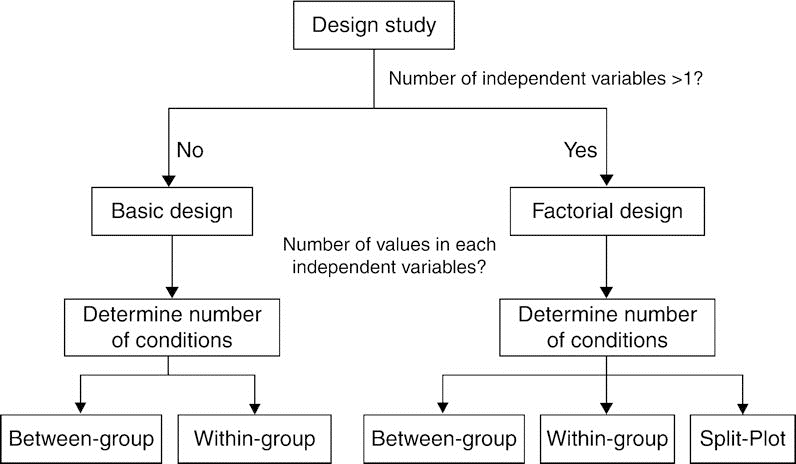
\includegraphics[scale=.5]{Hypothesis1}
\caption{Design study model}
\label{fig:designstudy}
\end{figure}

The difference between the two models is the fundamental test-structure, as seen in figure \ref{fig:designstudy}. In a between-group design, each participant is only exposed to a single experimental condition, meaning in this case he/she would only be playing the vehicle game with one of the controllers, not experiencing them both. In a within-group design each participant will utilize multiple conditions e.g. experiencing two polar opposite ways of controlling a game to establish which is the most user-friendly and convenient.

A within-group approach is usually less time-consuming due to decrease in the number of samples i.e. less test subjects needed to achieve a conclusive result \parencite{Lazar2010}.

Furthermore, Lazar argues that a Between-group construction creates a research setting where it is harder to obtain significant results, because data from different test subjects will have to be analysed under one common denominator. This indicates that a within-group construct would be preferred when choosing the strategic approach. Choosing a within-group construct is, however, not entirely without precautions.
\bigskip

\textit{Since the participants complete the same types of task under multiple conditions, they are very likely to learn from the experience and may get better in completing the tasks.}\parencite{Lazar2010}
\bigskip

This indicates that there is an increased risk of getting biased results, if user-experience is not taken into consideration. If a test subject is introduced to one control-system, and afterwards will try another as to compare the performance he/she may already be familiar with the conditions, and thus a reliable comparison cannot be substantiated. Lazar suggests changing the conditions e.g. altering the sequence of the test randomly per test subject, and furthermore changing the layout e.g. alternative racetrack can plausibly reduce the risk of getting biased samples. 


\subsubsection{Triangulation of data}
Whenever data is collected for any sort of experiment, risks of undermining the data by bias is always present. To prevent evident bias, many different approaches to minimizing the risk of bias can be initiated. 

One, more general, strategy to use, however, is that of data triangulation. The idea behind data triangulation is that by having multiple different data sets (as a result of having multiple tests) from each participant, it is possible to "precisely measure location" \parencite{Lazar2010}; 
in other words -  more accurately measure a tester's response to a product, for example.
\bigskip

An example of how triangulation can be used in practice is first by having the test subject do the experiment, while being observed. Then the test subject is asked about previous experiences (e.g. anecdotes) and their thoughts about similar products. And finally they are asked about future expectations of technology (or whatever subject is being researched).
\bigskip

From these three data sources, an overview of that tester's reaction to technology can be measured - A combination of how the person reacted during the experiment and how they responded to both the questions about past experiences and future expectations. This can give a relatively precise measure of how that person feels about a problem, compared to if they had just been handed a questionnaire, where they, themselves, should rate the product \parencite{Lazar2010}.
\bigskip

The purpose of using triangulation of data, is to minimize the risk of bias, by minimizing the risk of misinterpretation of data - just like it is hard to interpret the direction of a vector in math, from only a single point, it can be hard to interpret the intent of only a single set of data. Whereas multiple data sets (or point, in the context of vectors) will often have a more well defined "heading" (i.e. a user's reaction to a product, for example), thus making it easier to interpret accurately.

That being said, the use of triangulation does still not guarantee bias-free results, as data sources might be diverging, with the data covering different observations. When this happens, the test can still be valid, and triangulation still feasible to some extent, but it is usually not possible to reach a decisive conclusion based on such data alone, which in turn means that further testing might be required if a definitive answer to a test is needed \parencite{Lazar2010}.


\subsubsection{Usability Test}
Testing the product during development is an important aspect of any development process. Usability testing of a prototype involves the user into the testing of the product to make sure that the product is developing in the intended direction, and also determines to which degree the requirements have been proper implemented in terms of functionality. User based testing is usually used to test layouts of user interfaces and other user related aspects of the product.

\noindent Usability testing of a prototype involves \parencite{Lazar2010}:
\begin{itemize}
\item testing prototypes that have only been built on paper (known as paper prototypes);
\item testing prototypes that look complete but have a human behind the scenes responding (known as the “Wizard of Oz” technique);
\item testing working versions of software before it is officially released;
\item testing software that has already been implemented in existing systems. 

\end{itemize}


\subsubsection{Preliminary Test}
The preliminary test is a test prior to the actual test of the implemented product. The test is an examination of the specific method for which the final test is conducted. It will illuminate the different aspects in terms of procedure and results and if the designated procedures are functioning as intended. 

What will be happening, is a preliminary replica of the designated test will be conducted, where instead of having focus on the specific acquired data results, the test is the actual data, from which will be examined to account for the success of the test structure.

\subsection{Test content} \label{sec:testcontent}
Here, the strategy of the methodology of the test will be described. 
The specific data acquiring methods, test setup, description of test approach, data sheets and the structure of the general test procedure.

\subsubsection{Goal}
The goal with the test is to accumulate data which can ultimately prove or disprove the problem statement and the list of requirements. As specified in the method chapter (\ref{sec:hypotheory}) a hypothetic test will be conducted with an experimental structure for which it is possible to define variables which can be investigated. Additionally, independent variables can be researched to account for different data outputs.


The variables cover the following data, for which outputs will be obtained:
\begin{itemize}
	\item Final problem statement
	\item List of Requirements
	\item Controller Functionalities
	\begin{itemize}
		\item Steering left and right
		\item Acceleration
		\item Braking and/or driving reverse
		\item Gear shift
		\item (optional) action button
	\end{itemize}
\end{itemize}

Additionally, the test will allow the users to provide feedback thus enabling the possibility to get data that reflects the level of success for which the product has been developed and implemented. 

\subsubsection{Target group}
Non probability sampling will be utilized. 
It is a subset of people whom represent the general population of people that is familiar with vehicle games as defined in the method chapter (\ref{sec:approach}).
A preferred amount of 20 test subjects will allow for a diverse sampling for which, plausible data can be triangulated to allow for validation in terms of the acquired data.

\subsubsection{Test materials}
The test will be conducted with the use of the game Dirt 3(XX INSERT DIRT 3 INFO IN THE ANALYSIS). 
The game has all the functionalities as specified in the list of requirements, and can therefore serve as a platform to test the controller.
To compare the product with the SOTA controllers, an Xbox 360 controller will be utilized to allow comparisons of the two.(XX DEFINE WHY XBOX CONTROLLER IS SUFFICIENT)

\subsubsection{Observation}
While playing, the test subject(s) will be observed. 
The following observations will be made throughout the test subject’s gameplay in order to account for similarities or differences of the two controllers. 
Functions are defined as the controller functionalities. 
The observations are based on noticeable events and does not cover log of the data thus it will be accounted for if the test subject is experiencing any of the following function complications.

\begin{itemize}
	\item Function delay\newline
		The general response rate from the subject enabling a specific function, to when the actual controller function is 				activated.
	\item Non responsiveness of functions\newline
		The response for which, utilizing a function is either non responsive or behaving anyway that differs from the SOTA 			controller which complicates the gameplay.
	\item Activation of functions\newline
		The activation of any controller functionality which is not activated when desired at any point.
	\item Noticeable complications when enabling consecutive functions.\newline
		Complications that might occur while enabling several controller functionalities in a consecutive order or 						simultaneously.
	\item Noticeable difficulties when handling and utilizing the controller.\newline
		If the test subject experienced any problems with the usage and handling of the controller in terms of movement and 			gestures.
\end{itemize}


\subsubsection{Interview} \label{sec:interview}
An interview will be conducted after the consecutive game tests. 
An interview is utilized because of the use of open ended questions which will allow the users to give detailed answers, as opposed to questionnaires with open ended questions which might result in very limited response.  
The interview will cover the following subjects.

\begin{itemize}
	\item Questions that will substantiate the observations.
	\item Questions that will account for unforeseen opinions, comments or thoughts from the test subjects.
\end{itemize}

 For the full list of questions see (XX APPENDIX QUESTIONAIRE).
 
 
The interview will plausibly indicate whether or not the observed notations are applicable for the accounted observations.
This means that the specific observed complications will be compared to the test subjects own opinion of the experienced plausible complications thus proving or disprove the accuracy of the observation. 
Additionally, the interview will allow the test subjects to give detailed information towards plausible thoughts and opinions of the product in order to evaluate the success of the controller in terms of requirements and ultimately answer to the final problem statement.


\subsubsection{Test setup}
The method for the test is conducted with the structure of a within-group design as specified in the method chapter \ref{sec:hypotheory}.
\bigskip

The test will be divided into two separate test phases for which each subject will be asked to conduct each one consecutively. 
Thereafter an interview will be conducted. 
Each test subject will either start to play with the developed product or with the SOTA product. 
After each test, the sequence will switch, to gain varied data of the two controllers to minimize plausible bias, by starting with one specific controller for each test.
\bigskip

The second test phase will be the user playing the same track(s) in Dirt 3 where the other controller is utilized. 
Here the user is able to draw comparisons between the two controllers thus making it likely to obtain data of the plausible similarities or differences of the two controllers.
\bigskip

Lastly as specified in interview(\ref{sec:interview}) an interview of the test subject will be conducted. 

\subsection{Usability test}
After setting up for the test, the group conducted a final usability test, in order to ensure that everything worked as intended, and no elements of the testing room interfered.
This was done by having group members conduct the test a few times, leaving the data collection out. 
The group systematically tested each of the functions as thoroughly as possible, and in doing so, discovered a few issues.

\subsubsection{Problems with gear shift}
During the usability testing, some problems were encountered with the gear shift function.

The gear shift was supposed to be activated when the BLOB, marked during the setup, were moved within a box on the screen - the upper part should shift the gear up, the lower part should shift it down, while the center would be ignored, giving the user room to "enter". 
This, however, proved to be an issue - as the gestures required to execute the function were rather difficult to perform, while also maintaining control of the steering wheel. 
Additionally, unresponsiveness were encountered on several occasions - even with a second person handling the gear shift functions (to eliminate the possibility of the problem being caused by the difficulties of activating the function), it seemed to activate irregularly i.e. the gear would sometimes shift up, when trying to shift down, activate on its own, or not at all.


So with testers signed up for testing within the hour, the group decided to exclude the gear shifting all together, ensuring the test was working at the scheduled time period, rather than postponing the test, risking not being able to get enough testers. 
This course of action removes a required element from the software product though, and as such, it is something which should be reworked during the redesigning phase.

\subsubsection{Camera shift difficulties}
Some problems were encountered, when the group stress-tested the program by trying out the camera shift action, while accelerating and turning, namely that one of the inputs would simply be ignored - It became apparent that a maximum of two inputs could be activated, therefore the camera change function were changed slightly - it now requires the wheel to be in a neutral position, which therefore doesn't allow the speed to be in- or decreased while changing cameras, which were deemed a reasonable compromise.


During the actual testing, it became apparent that the limits, which marks the area where the camera view will not be changed, were perhaps slightly too small, as many people accidently changed camera view, while trying to steer due to the fact that the wheel had no center attachment, and as such would be moved around, passing the boundaries on several occasions.
\subsection{Procedure}
Here, the procedure of the test is explained in detail. 
The general data from the test, the description of the test course and the specified guidelines for the interview and observations of the test persons will be presented in the following sub-chapters.


General data about the test is seen here below, such as amount of participants, time and placement:
\begin{table}[!htb]
\begin{tabular}{l l}
Amount of participants: & 12 participants.\\
 & \\
Test subject data: & Convenience sampling: Aalborg university students.\\
 & \\
Estimated length of test: & 15-20 minute per test subject.\\
 & \\
Test location: & Aalborg University, conference room.\\
 & \\
Date of test: & 10/12 – 2013\\
 & \\
Estimated time of day: & 13:00 – 16:00\\
\end{tabular}
\end{table}


\subsubsection{Procedure: Test setup}
In the test setup, four persons were present for each test, i.e. 1 test subject, 2 observers and one person assisting the test subject. 
The test subject was placed on a chair with a laptop on a table in front of him/her. 
The webcam on the laptop was pointing towards the test subject, such that it would capture the gestures performed by the test subject while the test subject would also be able to see what was happening on the screen. 
At figure \ref{fig:testsetup} an illustration of the placement of the two observers can be seen. The two observers were placed slightly behind and to the side of the test subject to prevent any influence on the test subject by the observers. 
The observers were placed by a table with an assisting laptop and papers for notation. 
During the execution of the tests for each test subject, the assistant of the test subject would stay in the background, when not needed, in order to also prevent any influence on the subject.

\begin{figure}[!htbp]
\centering
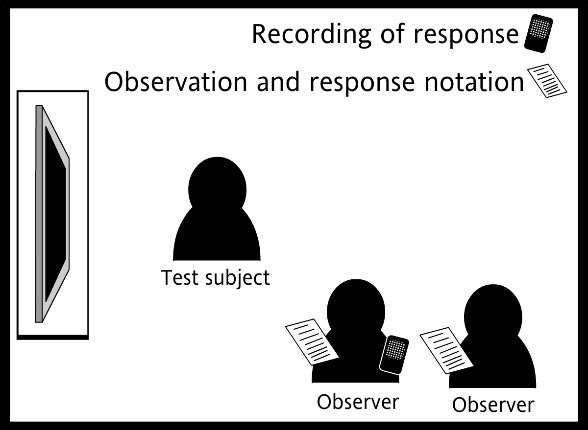
\includegraphics[scale=1]{Procedure1}
\caption{Test phase description} \label{fig:testsetup}
\end{figure}

Other individuals, such as subjects waiting for their turn to be tested and spectators, presented during the testing of one subject, were placed further away in the background, to prevent them from getting in the way.


\subsubsection{Procedure: Test materials}
A listing of all materials used during testing of all test subjects is presented here. 
This list excludes materials such as tables and chairs:
\begin{itemize}
\item Two laptops – one used by the test subject to play with the controllers and one for recording and noting observations (will be explained in the subchapter Test execution (\ref{sec:testexecution}))
\item The prototype controller described in the implementation (chapter XX)
\item Xbox 360 (SOTA) controller compatible with pc.
\item Notation paper-sheets – This includes blank papers for observations and papers with guidelines for the interview of the test subject (see Appendix XX for interview guidelines)

\end{itemize}

This list includes all materials used by the test subject and/or the two observers described above. 
To elaborate on the prototype controller, it includes both the wheel-like controller and not the yellow sponge as the functionality of gear shifting was removed (described in usability test chapter XX).

\subsubsection{Procedure: Test execution} \label{sec:testexecution}
The test execution itself is parted into sequences, one for each test subject. 
Every test subject going through a testing sequence did the same things, but one difference between each half of the test subjects, was the order in which they went through the parts of the sequence.


Taking a starting point from the first test subject, the sequence started out by placing the subject in the chair in front of the computer, as described above. 
Before the actual testing started, the assistant to the test subjects had made sure that the prototype controller had been setup correctly through the implemented software. 
The prototype wheel-like controller was then given to the subject, and the way to use the controller was explained. This includes telling the test subject the following:

\begin{itemize}
\item To accelerate the car in the game that the subject was now about to try, the wheel controller had to be moved towards the laptop/camera.
\item To brake or reverse, the wheel should be moved directly away from the camera.
\item To turn the car, the wheel should be rotated left or right accordingly.
\item To change the camera viewing angle in the game, the controller should be moved perpendicular to that of acceleration and braking, i.e. move the wheel left or right. Any of the two directions would activate the same function.
\end{itemize}

The test subject was then given the chance to try to use the acceleration and braking functions before testing, to give them the possibility get a feeling of how much they had to move the controller forward or backward to activate the functions. 
When the subject was ready for the first attempt to drive through the race track in the game, the game was started and the subject would then try to reach the end of the track as good as possible. 
During this first drive-through of the track, the collected data is based upon observations of the following content:

\begin{itemize}
\item Subject opinions/comments
\item Misc. actions or incidents, which were deemed noticeable by the observer(s) to be accounted for.
\item Function delay which affected the gameplay.
\item Non responsiveness of functions that affected the gameplay.
\item Difficulties activating functions that affected the gameplay.
\item Difficulties with enabling consecutive game functions.
\item Difficulties with controller movement and handling.
\end{itemize}

When the subject had finished this first try, the observers noted the time the subject took to complete. 
The subject assistant then switched the prototype controller with the Xbox 360 controller, while the two observers asked the subject some questions following the guidelines described in the material sub-chapter. 
When all questions were answered, the test subject was then explained how to use the Xbox controller in the same way as the prototype controller with respect to what buttons on the controller did what. 
The subject could then start the race over a drive through the track, but now with the new controller. 
During this drive-through, the observers again noted any observations like before. 
At the time the track was completed, the time of completion was noted again and the test subject was then asked the same questions, now with respect to the Xbox controller. 
\bigskip

This sequence of testing one test subject was repeated for all of the participants but every other subject started using the Xbox controller followed by the prototype controller.
\subsection{Results} \label{sec:results}
This section covers the results which have been collected.


\subsubsection{Quantitative data}
The following quantitative data has been accounted for:

\begin{itemize}
\item \textbf{Subject no:} Specifies the number of the participant.
\item \textbf{Controller sequence:} Indicates the sequence for which the contestant played a lap with either of the controllers first and then afterwards the other.
\item \textbf{Product time:} Describes the time for which the lap has been completed with the developed product.
\item \textbf{SOTA time:} describes the time for which the lap has been completed with the Xbox controller (State of the Art controller).
\end{itemize}

\begin{table}[!htbp]
\centering
\begin{tabular}{| l | c | c | c |}
\hline
\textbf{Subject no.} & \textbf{Controller sequence} & \textbf{Product time: min/sec} & \textbf{Sota time:}\\
\hline
\# 1 & PRODUCT $ \rightarrow $ SOTA & 3:28 & 3:11\\
\# 2 & SOTA $ \rightarrow $ PRODUCT & 4:58 & 3:13\\
\# 3 & PRODUCT $ \rightarrow $ SOTA & 5:14 & 3:05\\
\# 4 & SOTA $ \rightarrow $ PRODUCT & 4:49 & 3:04\\
\# 5 & PRODUCT $ \rightarrow $ SOTA & 4:46 & 3:07\\
\# 6 & SOTA $ \rightarrow $ PRODUCT & 3:29 & 3:09\\
\# 7 & PRODUCT $ \rightarrow $ SOTA & 4:03 & 3:11\\
\# 8 & SOTA $ \rightarrow $ PRODUCT & 3:59 & 3:03\\
\# 9 & PRODUCT $ \rightarrow $ SOTA & 3:45 & 3:05\\
\# 10 & SOTA $ \rightarrow $ PRODUCT & 4:29 & 3:17\\
\# 11 & PRODUCT $ \rightarrow $ SOTA & 3:37 & 3:11\\
\# 12 & SOTA $ \rightarrow $ PRODUCT & 4:54 & 3:21\\
\hline
\end{tabular}
\caption{Description of control sequence and recorded lap records} \label{tab:timemeasurements}
\end{table}


\subsubsection{Qualitative data}
The qualitative data covers the observations of the gameplay from each of the test subjects. Both from the gameplay using the constructed artifact, but also observation notes of gameplay with the SOTA controller.
Also, the qualitative data covers recorded interviews of each test subject right after a lap with either of the controllers, which has been converted into text.

See appendix \ref{app:obs} for the combined list of observation results.


\subsubsection{Interview}
Full interview notes: appendix \ref{app:interview}.

After each lap with any of the controllers, the test subject is asked to answer questions, which concerns the following question templates.

\begin{enumerate}
\item Did you experience any Function delay that affected the gameplay?
\item Did you experience any Non responsiveness of functions that affected the gameplay?
\item Did you experience any difficulty activating game functions that affected the gameplay?
\item Did you experience any complications with enabling consecutive game functions (using functions together in context) that affected the gameplay? 
\item Did you experience any complications with the controller movement and handling that affected the gameplay?
\end{enumerate}

The answers which were obtained from the test subjects were recorded. 
Thereafter the answers from the test subjects are combined and placed below the identified relevant question.


\section{Discussion}

Throughout this discussion the project will be reflected upon, as a whole. This includes looking at the choice of alternative structure for the project, as to what occurred in this new form compared to the generally used structure. Additionally, there will be a discussion on what was achieved through the different steps of the project, e.g. the research, implementation and evaluation phases. All this discussion will ultimately lead to some pointers to how well the problem, formulated for this project, was solved, i.e. to what extends the problem was solved and what this can be used for.
\bigskip

The structure of the entire report was to emphasize suggestions of designs during development of, not only the product, but also the process of obtaining information and knowledge to form the final problem statements and the requirements. This method allowed the possibility to create several design templates that would plausibly suffice as a solution to the specified problem statement. Based upon the test results, there are no real indications towards the chosen design being the most efficient solution out of several suggestions. Although, by evaluating the test results, as to find the elements that were dysfunctional in any matter, it was possible to create a redesign of the implemented product, to plausibly suffice as the most efficient solution based upon the acquired research and test results.
\bigskip

The parameters of the list of requirements were clear; i.e. the design would have to be completed within the boundaries of, among other things, a standard webcam and e.g. ordinary household remedies such as cardboard and colored paper. The list of requirements is developed to be seen as parameters for which, if implemented, is successful to answer the final problem statement. There is, however, several methods for which each requirement can be implemented, and does therefore require speculations as to how the actual implementation has been constructed, and to what degree the success of said requirement is fulfilling its purpose of answering to the final problem statement. The requirements, describing general hardware and software does not count towards requirements which are subject for discussion, since the sheer development of the artefact is fulfilling the specified requirements e.g. that the controller must require a standard webcam.
\bigskip

The remaining requirements are, however, interpretations and conducted choices as to how each specific requirement are implemented. By interpreting the data, gained from observations and interviews, it was possible to interpret and deepen the understanding of how each requirement could have been conducted differently. The functionalities were e.g. defined as movement and additional functions such as gear shift and alternative camera angles. The outcome of the preliminary test indicated that our constructed solution to the gear-shift function was inefficient, therefore it was never tested, but interview answers indicates that it would have been a prohibitive feat to manage while steering the vehicle.
\bigskip

In accordance with the final problem statement the initial purpose of the project was to establish whether or not a controller could be created that would be comparable to an undefined SOTA-controller in terms of functionalities.
Through the strategy of the laid out test-methodology it was, among other things, recorded that the test subjects generally did comprehensively better with the SOTA-controller i.e. completed lap-time. This indicates that the comparison is imbalanced, meaning that a play through with the SOTA-controller is more effective i.e. the functionalities are advantageously implemented, compared to the created artefact. Such an outcome is expected from a general comparison between the two products; however, the intention of the product was not to be on par with a SOTA-solution, but merely to create a comparative product from relatively simple remedies. In this respect, it is assessed that the problem statement has been answered to a partial degree.	
\bigskip

Going through the process of this project and stepping towards an implemented attempt of a solution to the defined problem, formulated in the initial problem statement, and further specified in the final problem statement, several interesting areas and aspects of visual computing were revealed. Starting with the research gathered, to clarify the problem statement, several new ways of analysing, and processing, a video feed, previously completely/partially unknown to us, gave a much better understanding of what visual computing is, in its raw sense. Additionally the research opened up our perspective on what might actually be possible, when trying to reach for a webcam-only-dependent game controller that would be comparable with the more modern technological gaming platforms/controllers such as the State of the Art (SOTA) products i.e. in this case, an Xbox controller.
\bigskip

The acquired research found, led to designing of a plausible solution to the problem, different designs were developed, in order to widen the perspective of the possibilities to solve said problem statement. These designs all had a part to themselves, which made them unique, yet still all relevant as to how the functionality, required by the games, could be implemented. Even though they all had their differences, it still seemed like all of them would be able to utilize almost the exact same methods, in regards to visual computing (Image Processing and -Analysis), showing how many possibilities there are in visual computing. However, through the implementation it became clear that some of the methods were much more demanding in relation to time consumption, and required knowledge. This ultimately lead to an implementation phase, where some difficult choices had to be made regarding whether the prototype should be able to obtain user input easily and quickly, with the downside of being imprecise and dependant on environmental lighting.
\bigskip

Additionally troubling thoughts, from before the actual research began, was whether a final prototype could be made possible to use with an already existing game on the market, or if it would require a development of a new game. Moving towards the implementation of the prototype different ways of solving this problem were found, yet all of them seemed to rely on the same kind of communication between the software developed for the prototype and the other application, i.e. the racing game. As earlier described in the usability test \ref{sec:usability}, this communication did seem to suffer from some flaws, which, at that moment, showed to be a big obstacle when trying to make the game controller able to handle several different functions at a time. This resulted in a prototype with the disability of not being able to handle the user’s input for gear shifting, together with the other specified functions. Although it seemed that the test and evaluation of the prototype would be suffering from this disability, it still yielded positive data. This data has the potential of giving directions for what a further development of this prototype would need, in order to accommodate the requirements and functionalities revealed through the research.
\bigskip

During the implementation phase, this proved to be true, although some actions were difficult to implement - theories as to why these problems occurred, is explained in the Evaluation chapter, analysis results \ref{sec:analysisresults}, and will not be repeated here. The product-test brought some new issues to light; our testers had trouble using the controller, even with the removal of the gear shift function. 

Through the strategy of the laid out test-methodology it was among other things recorded that the test subjects generally did comprehensively better with the SOTA-controller i.e. completed lap-time. This indicates that the comparison is imbalanced, meaning that a play through with the SOTA-controller is more effective i.e. the functionalities are advantageously implemented compared to the created artefact.
Such an outcome is expected from a general comparison between the two products; however, the intention of the product was not to be on par with a SOTA-solution, but merely to create a comparative product from relatively simple remedies. In this respect, it is assessed that the problem statement has been answered to a partial degree.
\bigskip

“Can a vehicle game controller be created, using a standard web cam that utilizes visual computing with functionalities, that are comparable to state of the art game controllers in terms of functionality?”
\bigskip

The question of the final problem statement seeks to answer whether a game controller can be created using a webcam instead of specialized hardware. During the testing it was found that the general usage of the developed product was functional, but with general software issues which could have been modified, added or deleted as proposed in the re design section. 
Based upon the test and the general interpretation of the results it can be concluded that the game controller indeed can be created, using a standard webcam utilizing visual computing. However, the functionalities are interpretations of implemented functionalities of which has been implemented in a manner which was deemed as the best plausible design solution. These comparable functionalities are however, when evaluating the test results and the redesign, subjected to change to further improve the constructed usage of hardware and the developed software.

\section{Conclusion}
\textbf{Overall Purpose:} Repeat our main points of the project from beginning to end. Conclude on what we have learned; make it short and to the point.	
Don’t include anything new in this chapter.


\clearpage
%------------------------------------------------------------------------------
% BIBLIOGRAPHY
%------------------------------------------------------------------------------
\pagestyle{plain}
\label{bibliography}
\printbibliography[heading=bibintoc]

\clearpage
%------------------------------------------------------------------------------
% APPENDICES
%------------------------------------------------------------------------------
% once appendices are started we can't go back
% make sure this is the last include!!!
\appendix
\appendixpage
\addappheadtotoc

\section{Naïve Designs} \label{NaiveDesigns}

\subsection{Control a car through gestures} \label{nd1}
\subsubsection*{Naïve Design}

\begin{figure}[h]
\centering
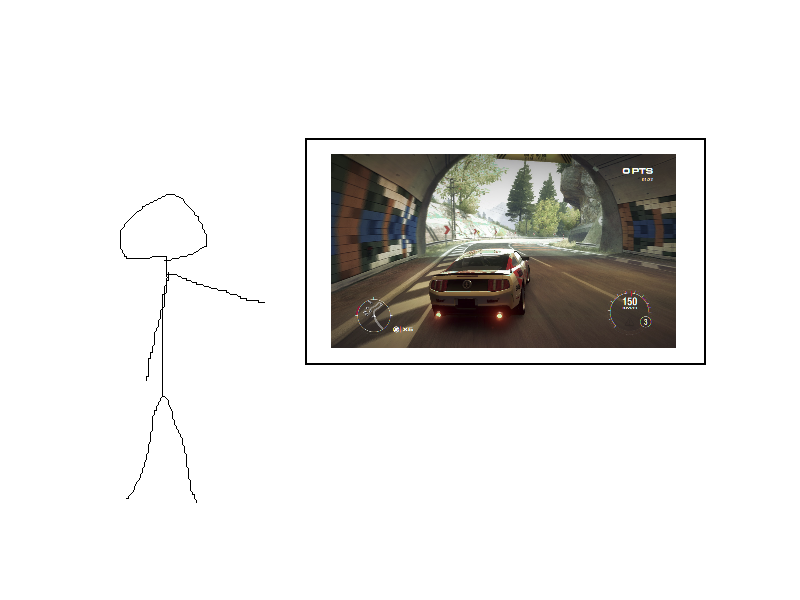
\includegraphics[width=5.5in]{NDesign1}
\caption{}
\label{fig:ndesign1}
\end{figure}

For this design we will use a standard webcam found in most laptops and other types of cameras that can send images to a computer. The idea is to make a vehicle controller, out of a camera, that can react to a user’ hand gestures and translate that into input for a vehicle based application or game. These gestures would translate to tasks commonly used in relation to vehicles, like speed up, slow down, change gears, hand breaking. The system should also be used to control the vehicles directions.


The idea here is to use hardware to get input from the user, however this hardware should not be specialized for gesture recognition, like a Kinect or Eyetoy. The hardware should be common to most computer users. The user should only need to install a piece of software and be ready to use gestures.


To make the camera recognize the different gestures some software will have to be implemented. This software will need to recognize the outline of the user and translate the gestures made by the user into commands for an application. The software should be able to recognize both static and moving gestures, for example, a static, flat hand shown to the camera could translate to a handbrake, or a fast movement of the right arm could translate to a hard turn to the right.

\subsubsection*{Design Analysis}
\noindent\textbf{Motivation} \newline
The motivation behind this concept is to replace the standard ways of using controllers with methods that does not require semi-expensive specialized hardware to operate.

This can be used to control applications like driving games without the need for specialized driving wheels, or analog joysticks, requiring only a basic set of hardware already available to most people who own a laptop. 
\bigskip

\noindent\textbf{Strengths and weaknesses} \newline
Strengths:
\begin{itemize}
\item This can make a driving game more approachable.
\item This can make a driving game controller less costly.
\end{itemize}
Weaknesses:
\begin{itemize}
\item Precision is very important. We do not want to end up in a ditch.
\item Input is not ergonomic.
\item Input lag becomes a much bigger concern.
\item Input methods are not intuitive.
\end{itemize}
\bigskip

\noindent\textbf{Target group} \newline
The primary target group for this concept is people who are confined to using specialized hardware for certain applications, like driving games or equally like-minded applications.
\bigskip

\noindent\textbf{What do you know / need to know} \newline
For this concept a good understanding of image processing is key. The product will be based on image processing to get its readings and translate into input. Precision is key to this product because it will potentially be used for precision operations like navigating a vehicle around a sharp turn.

We need to know how to translate data from a camera into input that the supported applications can understand and use.
\bigskip

\noindent\textbf{What to investigate} \newline
The main focus of the investigations is to figure out how much of this is possible and how much of it is possible using a standard webcam. We need to investigate if it is possible to get accurate readings from a camera that is reliable enough to be usable.
 
Another area of investigation is the industry’ perception of the idea. Is it even a good idea?

We need to know if the ergonomics of this approach is sustainable.
\bigskip

\noindent\textbf{Initial prototype / mock – up.} \newline
An initial prototype could involve using markers on the hands of the user and use one or more cameras to capture data. Software will be needed to translate the input, as well as a demo application involving navigation will be needed. This prototype will be used to answer what is possible with this concept and what needs improving. 

\pagebreak

\subsection{Controller blocks} \label{nd2}
\subsubsection*{Naïve Design}

\begin{figure}[h]
\centering
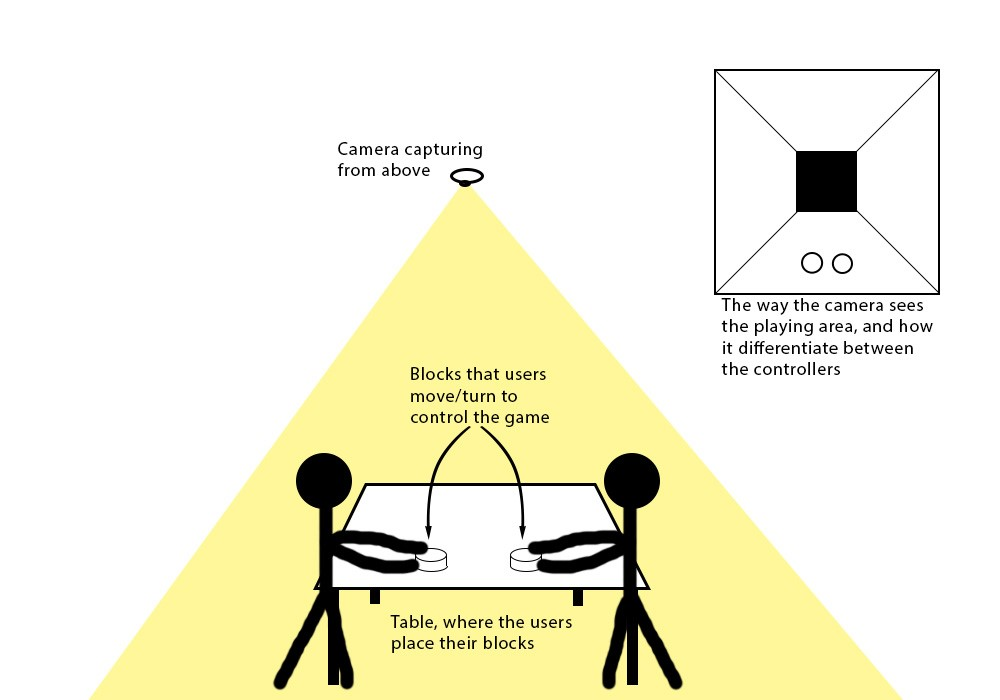
\includegraphics[width=5.5in]{NDesign2}
\caption{Game controller using blocks. By moving and/or rotating the blocks, the user can control the vehicle in the game.}
\label{fig:ndesign2}
\end{figure}
This idea would give the possibilities to both play as a single player and multiplayer (coop and versus). If we say that we are playing a car racing game, then we would use 2 blocks for each car that has to be controlled in the game. This means that one or two players can control each car. By moving the blocks around, the camera can detect their placement and then use this information to control the car in the game. If we have a table we are playing on, the camera would be looking down at the table from above. In the top right of figure \ref{fig:ndesign2} is illustrated how the camera could split up the playing field (where the users are moving the blocks around in) and in this way distinguish between which blocks control what car.

The control blocks would work e.g. as follows:
\begin{itemize}
\item Both blocks forward: the car accelerates
\item Both blocks back: the car brakes
\item Left block forward, right backwards: car turns to the right (and vice versa)
\end{itemize}
For other games that are not car racing, the blocks could be colored. With this addition, you could also rotate the blocks, which the camera could register by the colors on the blocks.

\subsubsection*{Design Analysis}
\noindent\textbf{Motivation} \newline
\noindent\textbf{problem} - This idea is based on a way to make a gaming platform, if you will, cheap, compared to other professional and popular platforms such as the Nintendo Wii, and Xbox Kinect, which both tracks movement performed by a user.
\bigskip

\noindent\textbf{Opportunities} - The idea here would give the possibility to play together (or against) your friends, as you can play multiple players at the same time. You can cooperate as two (or maybe even more) players in controlling one vehicle in the game, if you would like. This possibility is obtained by using two or more blocks on the board to control each vehicle.
\bigskip

\noindent\textbf{Inspiration} - The source of inspiration came partly from the previous idea (Race-making Game) where you are using blocks or something alike, to tell e.g. the car when to turn. An additional source of inspiration was the “music board” where you are using different kinds of blocks, and by placing them on a surface, you create different kinds of sounds. 
\bigskip

\noindent\textbf{Strengths and weaknesses} \newline
Strengths:
\begin{itemize}
\item Options for multiplayer gaming as well as single player
\item Cheap: only a webcam is needed, the blocks can be homemade
\item The blocks can both be moved around and rotated, giving several ways of controlling the vehicle
\item Social gathering, as the idea is to gather more people around the table and play together in the same room.
\end{itemize}
Weaknesses:
\begin{itemize}
\item Camera placement can be a bit problematic: camera has to see the blocks from above
\end{itemize}
\bigskip

\noindent\textbf{Target groups} \newline
As the main problem is focused on making a gaming controller of some kind, so target group will primarily be people already playing video games. This does not necessarily mean hard-core gamers. In fact, non-hard-core gamers would be of preference. Initially this idea might seem more appealing to the same kind of people that uses Nintendo Wii, Xbox Kinect or alike, as this idea involves having people in the same room when playing. Those kind of people might be families playing together once in a while, or friends gathering to play together in another way than LAN parties.
\bigskip

\noindent\textbf{What do you know / need to know more about?} \newline
\noindent\textbf{Visual computing} - Some knowledge needed to make this idea come true would be how visual computing actually works. The camera in this idea would need to recognize the blocks on the table and read how they are being manipulated to perform an action in the game. 
\bigskip

\noindent\textbf{Users} - The product of this idea especially has to be appealing to the target group in order to give them the satisfaction they would have gotten from using a popular gaming platform. This means that the controls have to be easily understandable and manageable as well as many other things, which would need research.
\bigskip

\noindent\textbf{SOTA} - At the moment it is unknown if there are ideas like this already developed. So far it is known that there is a device that utilizes something like this idea, but instead of controlling a vehicle in a game, the device provides sound and music according to what kind of block you place on a surface that reads the blocks.
\bigskip

\noindent\textbf{What would you be investigating?} \newline
\noindent\textbf{Image analysis and processing} - 
Using a webcam will provide a flow of images of the area in which the users will be controlling their blocks. These images need to be analyzed and processed in order for the software, that will be developed, to understand what the user wants the program to do. To be able to use the images like this research has to be done in the area of image analysis and processing.
\bigskip

\noindent\textbf{Initial prototype} \newline
For an initial prototype, it would be useful to focus on using one specific video game. Say we take a car racing game; the prototype would only have to focus on how to control a car in order to see if it is even possible to get near a product where the user would be able to control all kinds of vehicles.

\pagebreak

\subsection{Immersive Racing Game Experience} \label{nd3}
\subsubsection*{Naïve Design}
\begin{figure}[h]
\centering
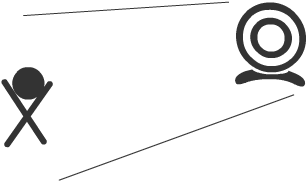
\includegraphics[width=5.5in]{NDesign3}
\caption{}
\label{fig:ndesign3}
\end{figure}
The theory behind (IRGE) is to use a static webcam to track your movement/face by recognition and thereby allowing enhanced immersive gameplay by the use of real like movement as required in the specific computer game.


By tracking the whole body you are able to navigate in the game, since we are going to make a vehicle controller based on the user we got many possibilities. We might focus on car games it would be obvious make the webcam track our movements like we were driving a real car. If time is on our side we might also make a controller for other kind of vehicles. 


This use of webcam movement tracking can generally be used in games that requires varied movement such as Racing games, First person shooters, puzzle games(Portal) and others, where the player act as a person with movement functionalities within the game itself.

\subsubsection*{Design Analysis}
\subsubsection*{Motivation}
Also as several of the other ideas the motivation for this one is not based on a particular problem that can be solved. Hence it is an idea that is specifically targeted for entertaining purposes only.


The theory is to enhance immersive gameplay by the use of real life movements in the specific computer game, where it is required.


The opportunity with this idea is to enhance the experience by being the subject which is used to control the in-game player in terms of movement.


\subsubsection*{Strengths and weaknesses}
Strengths:
\begin{itemize}
\item Could contribute to the already evolving technology of virtual reality.
\item Would be a cheaper alternative to more complicated ways of immersion, such as the Wii, provided that the user has enough space.
\item Healthiness. The user is able to get some sort of exercise while playing a game.
\item Could be a multiplayer experience.
\item Has the potential to be fun to make.
\item Has the potential to be fun for the users, although that would be subjective.
\end{itemize}
Weaknesses:
\begin{itemize}
\item Requires a large amount of space to interact in.
\item Could limit social aspect of games.
\item Most people do not have the required equipment and space to make this game fully functional.
\end{itemize}


\subsubsection*{Prototype - Mock-up}
An early prototype for this concept could be a hallway with a screen and a webcam at the end. In the hallway could be obstacles that the user can hide behind as part of a game. Software will have to make to be made to translate the data from the camera into input to a demo game that we will borrow for the testing.
\bigskip

A prototype would clarify if users would like the idea of a racing game controlled by movements. A prototype could help show the technical limitations of this concept.


\subsubsection*{Target Groups}
The ideal target group for this solution is people who like to play games, but feel that the control options available are insufficient / uninspiring, and would like the games to be more immersive.


\subsubsection*{What do we know / what do we need to know more about}
We know that the concept is somewhat similar to that of the Kinect as far as movement goes. The innovative part of the concept is that the player will be able to see himself on the monitor, and will be able to drive the car around by using steering wheel movements, speed up and down movements and other kind of movements that are needed to control the car or options in the game.
\bigskip

The Kinect is a state of the Art product in this line of gaming, so it will, for obvious reasons, is natural to investigate how it works.


\subsubsection*{How much research has to be done in this area (from 1-5, where 5 is most)?}
\begin{itemize}
\item State of the Art: 4
\item Full body motion capture: 5
\item Perception: 2
\item Player motivation: 5
\end{itemize}


\subsubsection*{Investigations}
For the user to be able to control the game via the webcam, a study upon how you analyze and process an image input from the camera has to be done. The focus here will be how to find and analyze an object/person in the picture and use the person’s movements and gestures to apply some action in the game.

\pagebreak

\subsection{Pointing controller} \label{nd4}
\subsubsection*{Naïve Design}
\begin{figure}[h]
\centering
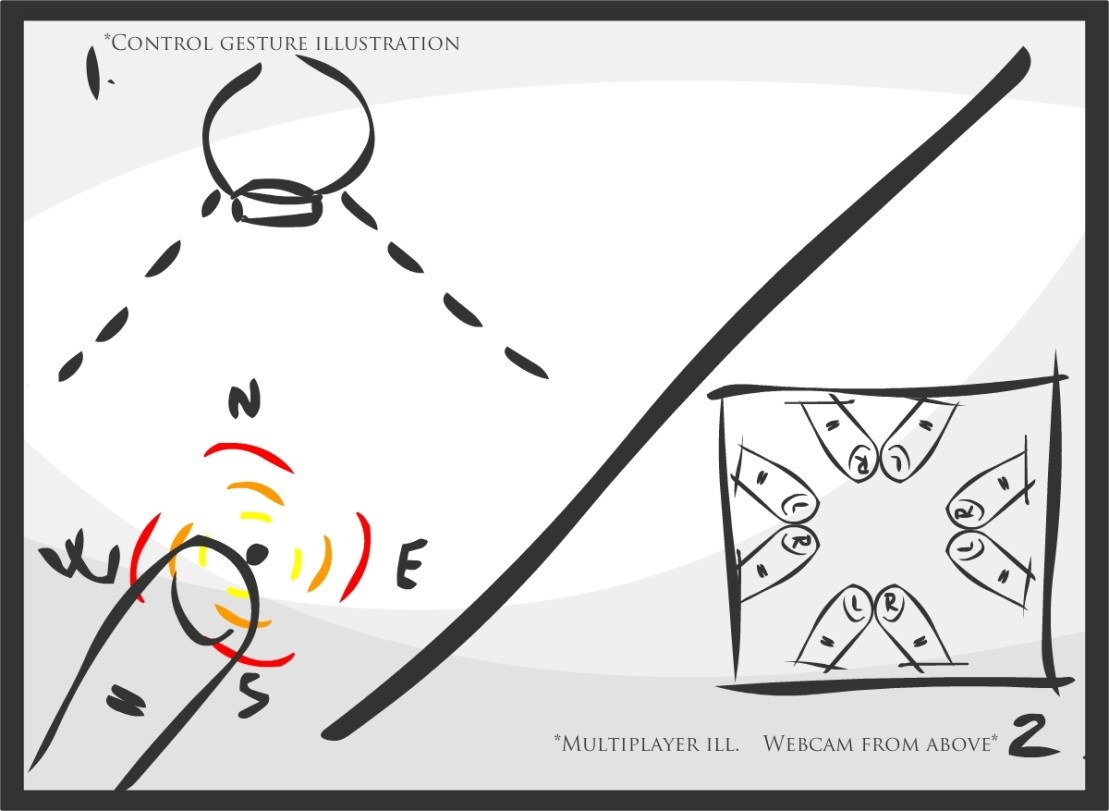
\includegraphics[width=5.5in]{NDesign4}
\caption{}
\label{fig:ndesign4}
\end{figure}

The idea behind this concept is to use a webcam to track finger(s) on a plain surface to register movement and functionalities of the designated game. By relocating the finger(s), depending on the game, the input will act accordingly to the specific game/functionality.
\bigskip

Also, to incorporate multiplayer functionality, several players can be recognised and because of limited movement to control the specific game, a single webcam would be adequate to keep track of (x) players.
\bigskip

Illustrates the finger movement, and predetermined possible movement/control functionalities of the setup. (Illustration \ref{fig:ndesign4}: Example 1)
\bigskip

The rotation of the players, can be adjusted down to the individual to address the angle of the screen and the angle of control that the specific player so desires. (Illustration \ref{fig:ndesign4}: Example 2)


\subsubsection*{Naïve Design}
\subsubsection*{Opportunities}
The idea is based on visual computing where there is no need for controllers. A simple webcam and a plain surface will suffice to create the specified game experience where you control the functionalities with the tip of your finger(s). This method of controlling the vehicle can be modified to combine alternative methods of controlling the game, but also customization of alternative controlling methods possible since there are buttons to limit the possibilities.

\subsubsection*{Strength/Weakness}
The \textbf{strength} of the design is first of all the simple hardware requirements which is easy accessible and plausibly with a very simple setup. 
\bigskip

Also, by not limiting ourselves to a controller which is already developed with a limited amount of functionalities, we are able to imitate all of the preexisting functionalities and exceed those, since there are no button limits, but rather space limit depending on the single player/multiplayer experience.
\bigskip

The \textbf{Weakness} of the design is that by utilizing a camera for tracking movements, you do not get any sort of haptic feedback under any circumstances during the experience.
\bigskip

Also, it is possible that the amount of functionalities that must be present in order to be comparable in terms of functionalities with other game platforms, is too much to cope with, since there are no visual interface lying on the surface while you are playing. Only a visual interpretation of the game mechanics that might appear on the screen.

\subsubsection*{Target groups}
The target group is people whom are interested in playing vehicle games on consoles and plausibly already do so. Preferably we are able to aim at people who are actually playing/performing vehicle gaming on a higher level, in order to research whether or not our take on a plausible alternative to preexisting methods is even a possible solution.

\subsubsection*{What to know}
\noindent\textbf{Theory/Research} - First of all we need to figure out what makes a vehicle game the preferred experience with the different controllers in order for us to establish requirements towards, what our product should be able to do and contain.
\bigskip

Furthermore, we need to establish a base of knowledge of the vehicle games in order to figure out which functionalities our product should have. Lastly, we must of course research on how to create such controller for it to be able to function to a plausible large number of games, where the controller would be equally efficient as the preexisting. 
\bigskip

\noindent\textbf{Theory/Research}\newline
\noindent\textbf{Users} - First of all we must establish criteria towards what the users think that the product would need in terms of design and functionality. Also, it would be plausible that the users are so used to “regular” controllers when playing vehicle games, so perhaps, also try a separate target group of people who do have non to little experience with vehicle games to establish a measurable amount of data of the user experience within both groups.
\bigskip

\noindent\textbf{SOTA} - The state of the Art within this matter is the pre-existing controllers on the market. The Kinect controller, the PS controller, Wii and the special developed wheels to emulate the driver experience.

\subsubsection*{What to investigate}
First of all we must investigate the image processing technology behind the idea. What we are able to do and how we can utilize that specific technology.
\bigskip

Next we must investigate the preexisting controllers to delimit ourselves to how we can make the product “comparable with other gaming platforms”. What should our product we able to do, can it be implemented, and how can we improve on the matter?

\subsubsection*{Prototype}
The prototype would most likely be an alternative to the pre-existing controllers in terms of key-functionality. We could possibly argue that we have created an alternative method of controlling vehicle games, but since it’s a different approach – there would be both advantages and disadvantages which would probably be evaluated individually by the test subjects of the evaluation.
\bigskip

The success criteria would be if the product would suffice when comparing the established requirements and still be functional to a satisfaction of the users, but that cannot be speculated upon before the specific requirements for the success criteria is established.

\pagebreak

\subsection{Object-controlled Visual Processing} \label{nd5}
\subsubsection*{Naïve Design}
\begin{figure}[h]
\centering
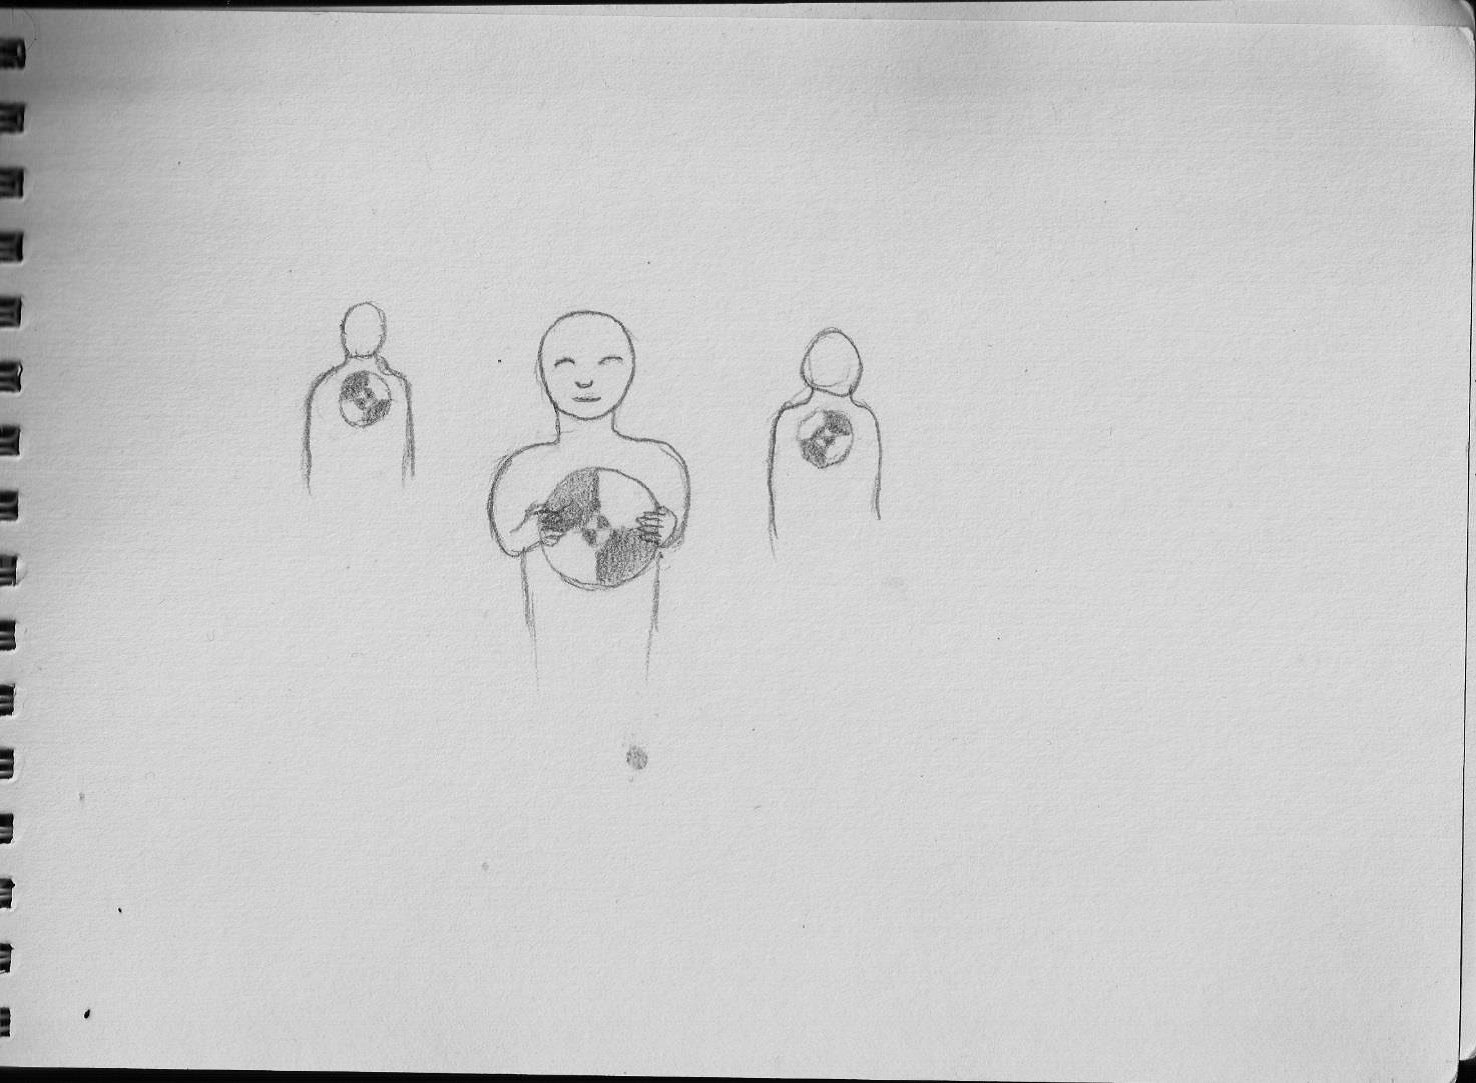
\includegraphics[width=5.5in]{NDesign5}
\caption{}
\label{fig:ndesign5}
\end{figure}

The idea revolves around a multicolored - or shape-recognizable object that can be moved around in front of the webcam to create a motion capture-device that can be used as a logical vehicle controller e.g. a plate as seen in the image for controlling a car or boat etc.
\bigskip

The objects are going to have some sort of pattern on them to make them easier recognizable for the camera. Due to this pattern, it should be easy for the camera to pick up side-to-side as well as up-down movement, rotation, and forwards and backwards movement. It also makes it easy for several people to use the device at the same time, allowing for potential multiplayer games, or collaborative work.
\bigskip
 
The currently State-of-the-art products out there such as Kinect, PlayStation Move or Wii only allows for 2-3 players simultaneously. So maybe we will be able to create a cheap alternative to those optional products that are furthermore able to sustain more players. Maybe we could also enable multiplayer online, so people might be able to pick up their plate and join the game with an avatar that reacts to the object’s movement.
\bigskip
	
In order to make this, knowledge about image processing needs to be known. However because the pattern the camera should recognize is a pre-defined static object, it should prove less of a challenge than with a varying object such as a human hand.

\subsubsection*{Design Analysis}
\subsubsection*{Motivation}
The concept behind this idea, is replacing the traditional mouse, with a wireless (and powerless) solution to be able to play vehicle games in an interactive, logical and intuitive fashion. 

We are motivated by the fact that products such as the Wii or Kinect seldom can sustain more that 2-3 players, and usually only come with 2 controllers, extra controllers can be purchased, but they usually cost a lot.

\subsubsection*{Strengths / weaknesses}
Strengths:
\begin{itemize}
\item Conceptually, the user would be able to use this 'mouse' from a rather great distance (though with diminished accuracy, as a side effect).
\item The physical aspect of the mouse could simply be a sticker, or something similar carrying a 	specific pattern, thus removing the need for a power source.
\item The number of players could be limited only by the restrictions of the game.
\end{itemize}
Weaknesses:
\begin{itemize}
\item The accuracy of the device is highly dependent on the skills of the user
\item Depending on the quality of the webcam, distance could very quickly become an issue for 	accuracy, as coding can only do so much.
\end{itemize}

\subsubsection*{Target groups}
The target group could be anyone who are interested in playing interactive games. 

\subsubsection*{What do you know / what do you need to know?}
For this product, a strong knowledge of image processing is key:
\bigskip

A) Knowledge of how to capture, record and convert a specific pattern (like the ones in the illustration) is required, in order for the program to reliably record the movement of that specific object, and not random background objects.
\bigskip

B) Knowledge of converting the data from A) into movement on the computer screen is needed - This could further be expanded upon, to allow for different settings (for different programs).

\subsubsection*{What would you be investigating?}
The main focus would be investigation regarding image capturing and processing.
\bigskip

Additionally we would need to gather some information regarding how web cams work, how the different types differ from one-another, and how this will affect the program - And how (if possible) to counteract this.
\bigskip

Networking would also be required to investigate if we were to implement an online solution. 

\subsubsection*{What could be an initial prototype / mock-up?}
An initial prototype / mock-up are not easy to make, as the solution is rather simple. One solution, however, could be to create a functional program, with only limited actions available (such as simply moving the mouse around, using image capturing.

\pagebreak

\subsection{Race-making game} \label{nd6}
\subsubsection*{Naïve Design}
\begin{figure}[h]
\centering
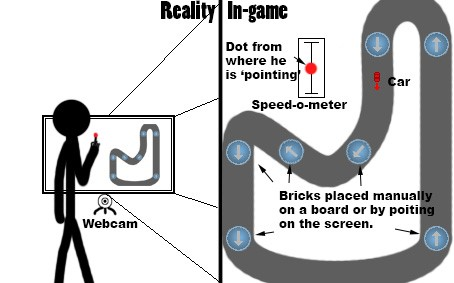
\includegraphics[width=5.5in]{NDesign6}
\caption{}
\label{fig:ndesign6}
\end{figure}

This idea is inspired by some of the racing tracks made for kids to build. You put the track together, and then you had a controller that could only control the speed of your car and nothing else. The goal was then to try and keep your car on the track, while still going at a maximum speed.
\bigskip

Of course what we should be explaining here is the controller, not the game itself. The controller has a board (not in the above picture), where you place down the bricks as “points” where you would like the track to go. The game then connects these points with lines, and there you have the track! This would use image processing to figure out where the bricks were placed.
\bigskip

You then use your finger to control the speed of the car, trying to make it go fast, but not too fast. You need to put a colored thing on your finger so the camera can see where it is placed.
\bigskip 

Note that this idea could be combines with some of the next ideas explained, and the control schemes could be altered to give you more control of the car.

\subsubsection*{Design Analysis}
\subsubsection*{Motivation}
This idea has roots in our childhood, and because of that it is something that we can relate to.
\bigskip

The game itself isn’t too complicated, with the hardest part probably being how to connect the dots to form a track, and making the car controls feel nice. The image processing part of it should be fairly simple.
\bigskip

This idea could also potentially require us to build a table of some sort for the bricks to be placed on. This means that there will also be some work in creating something physical, which some group members might like.

\subsubsection*{Strengths/weaknesses}
Strengths:
\begin{itemize}
\item The idea is something we can relate to.
\item Could be cheaper than buying an actual racing track.
\item Allows users to be creative by being able to create their own things with the provided material.
\item The idea itself is fairly simple.
\item Allows for social interaction.
\end{itemize}
Weaknesses:
\begin{itemize}
\item Could potentially require 2 cameras, however this can be fixed by using the board where you place the bricks as the “control-space” as well.
\item We’re not sure yet exactly how we can give the user the ability to create the track themselves yet.
\item Requires quite a bit of programming, might not be fun for all members.
\end{itemize}

\subsubsection*{Target group}
The target group would be anyone who plays games. Younger people might be a greater target group however, since they might’ve played the physical version of the game, and has some nostalgia when it comes to the game.
\bigskip

The game should be really simple and intuitive to use, so you don’t need a lot of technological expertise to use the product.

\subsubsection*{Knowledge}
We know for a fact that some students have made tables that are able to detect objects on top of it before, so some research has already been done in this area, and we’ll have some other products to compare ours to. The same has been done with color recognition.
\bigskip

In order to create this idea, we would need knowledge about image processing to create the controlling features. We would also need knowledge about how to create the actual game. This could be done in a lot of programs such as Unity, Flash, Processing and more. We could potentially also create it from scratch using c++, however this would most likely not be preferred.
\bigskip

We also need knowledge about vectors and vector calculation in order to create the track, and some knowledge about 2d physics, to make the car act in a way we want. However a program such as Unity already has a physics engine, potentially saving us time.
\bigskip

We can make loads of prototypes of this idea, and it has a lot of “steps” on which we can test the game. We can test the initial color recognition without the need of anything else, we can test the creation of the track without the need of anything else, and we can test the car ‘mechanics’ in a way without the need of much, except a track to follow.

\pagebreak

\subsection{Tabletize your computer!} \label{nd7}
\subsubsection*{Naïve Design}
The idea for this design is, using a standard webcam, simulating the rotation measuring devices of modern tablets and smart phones, allowing computer users the same intuitive means of controlling games.
\bigskip

As the webcam is recording, edges will be recognized (using image processing), and the movement of said edges will be converted into movement on the computer - In other words, movement within the captured pictures will be replacing the tilting sensors of the tablets and smart phones.

\subsubsection*{Design Analysis}
\subsubsection*{Motivation}
The motivation behind this concept, is to create software, that will allow a webcam to replicate the tilting and rotation sensors ordinarily found in e.g. tablets and smartphones. This would allow desktop and laptop computer users to immerse them selves in similar games - ie. games where the controls are more intuitive than simply using the WASD movement keys, for example.

\subsubsection*{Strengths and weaknesses}
Strengths:
\begin{itemize}
\item Allows for a more immersive experience
\item Expands the range of games available to computer users even further.
\item Could possibly be utilized for other purposes, where a tilt sensor could be useful.
\end{itemize}
Weaknesses:
\begin{itemize}
\item Hardware not built for this kind of action, unless using an external webcam.
\item Potentially hard / impossible to do general calibration, causing the device to needing 	recalibration after either every  game session or after every time it is moved from location to 	location.
\item Unless using external webcam, the setup can be both heavy and cumbersome, making the 	device less intuitive than the alternative, thus defeating the point.
\end{itemize}

\subsubsection*{Target group}
What do we know / what do we need to know more about:

We will most likely be using openFrameworks (C++ coding) to process the images into movement data. What we need to know is, how to convert the stream of images from the webcam into usable movement data ( ie. how to detect the movement in the images reliably). Furthermore we need to convert this data into actual movement in a game.

\subsubsection*{Investigation}
We will need to investigate similar, professional, solutions - sort of like the tablets and smartphones, but we should try to see if we can find someone who have done the same - without the use of tilt-sensors.
\bigskip

We will need to research a lot of image processing, and figure out how we're going to approach the movement - record - movement process (ie. recorded movement -> data -> output movement), and how much movement should account for how much movement on screen. 

\subsubsection*{Initial prototype}
An initial prototype is not easy to do, as it is highly software based, and thus will more or less be finished, once an initial prototype is ready for testing. "Simulations" (or Wizard of Oz-experimentations) could be used, however, as this would give us some idea of how the program will work and feel for the users, while being very time efficient.



\clearpage
\section{Testing-Time measurements} \label{app:time}
Acquired lap completion data.

\begin{table}[!htbp]
\centering
\begin{tabular}{| l | c | c | c |}
\hline
\textbf{Subject no.} & \textbf{Controller sequence} & \textbf{Product time: min/sec} & \textbf{Sota time:}\\
\hline
\# 1 & PRODUCT $ \rightarrow $ SOTA & 3:28 & 3:11\\
\# 2 & SOTA $ \rightarrow $ PRODUCT & 4:58 & 3:13\\
\# 3 & PRODUCT $ \rightarrow $ SOTA & 5:14 & 3:05\\
\# 4 & SOTA $ \rightarrow $ PRODUCT & 4:49 & 3:04\\
\# 5 & PRODUCT $ \rightarrow $ SOTA & 4:46 & 3:07\\
\# 6 & SOTA $ \rightarrow $ PRODUCT & 3:29 & 3:09\\
\# 7 & PRODUCT $ \rightarrow $ SOTA & 4:03 & 3:11\\
\# 8 & SOTA $ \rightarrow $ PRODUCT & 3:59 & 3:03\\
\# 9 & PRODUCT $ \rightarrow $ SOTA & 3:45 & 3:05\\
\# 10 & SOTA $ \rightarrow $ PRODUCT & 4:29 & 3:17\\
\# 11 & PRODUCT $ \rightarrow $ SOTA & 3:37 & 3:11\\
\# 12 & SOTA $ \rightarrow $ PRODUCT & 4:54 & 3:21\\
\hline
\end{tabular}
\caption{Description of control sequence and recorded lap records} \label{tab:timemeasurements}
\end{table}

\noindent\textbf{Subject no:} Specifies the number of the participant.


\noindent\textbf{Controller sequence:} Indicates the sequence for which the contestant played a lap with either of the controllers first and then afterwards the other.


\noindent\textbf{Product time:} Describes the time for which the lap has been completed with the developed product.


\noindent\textbf{SOTA time:} describes the time for which the lap has been completed with the Xbox controller (State of the Art controller).
\clearpage
\section{Testing-Observation notes} \label{app:obs}
The left brackets cover the observations notes for the laps where the test subjects used the constructed controller.

The right bracket covers the noted observations, where the Xbox controller (state of the art) was used.

\begin{table}[!htbp]
\centering
\begin{tabular}{| p{3.4in} | p{2in} |}
\hline
	\textbf{Test Subject \# 1: Product} & \textbf{SOTA}\\
\hline
	\begin{itemize}
		\item Slight function delay
		\item Breaking was non responsive. Wheel was not forward enough to enable it.
		\item The wheel was placed very far forward, in order to accelerate.
		\item Random activation of the camera view change. Occurred +5 times.
		\item Over exaggerated the turning motion to turn.
		\item After practice, enabling the “change view” was improved and functional
		\item Change view happens for no reason.
		\item Camera change view is enabled by flipping the wheel over the shoulder.
		\item Subject quote: “shoulder hurts”
		\item Subject rarely breaks.
		\item No in-game crashes.
	\end{itemize}
	&
	\begin{itemize}
		\item Easier to control
		\item Faster function response
	\end{itemize}
	\\
\hline
\end{tabular}
\end{table}


\begin{table}[!htbp]
\centering
\begin{tabular}{| p{3.4in} | p{2in} |}
\hline
	\textbf{Test Subject \# 2: Product} & \textbf{SOTA}\\
\hline
	\begin{itemize}
		\item No noticeable braking during race
		\item Change camera is enabled several times on purpose during game
		\item Game was reset because of technical difficulties – not associated with product.
		\item Wheel (board) was tilted, excessively when car was out of control (things were going bad).
		\item Several occasions: Car was wobbling. Hard left, or hard right.
		\item Arms of subject are placed very low. Near thighs in the sitting position.
		\item Noticeable frustration of the test subject.
		\item Slight function delay
		\item Tried to enable “change view”. Nothing happened
		\item Lost control of the forward/backward mechanics  - Trouble activating them after the other.
		\item Kept arms straight, (wheel close to screen) while driving.
		\item Random change of view occurred 3-4 times.
		\item After in game crash, subject had difficulties getting control over the vehicle, getting back on track. Forward/backward \& turning.
		\item Change of view was activated once on purpose.
	\end{itemize}
	&
	\begin{itemize}
		\item Several occasions: Car was wobbling. Hard left, or hard right.
		\item In game crash
		\item Over eager
	\end{itemize}
	\\
\hline
\end{tabular}
\end{table}


\begin{table}[!htbp]
\centering
\begin{tabular}{| p{3.4in} | p{2in} |}
\hline
	\textbf{Test Subject \# 3: Product} & \textbf{SOTA}\\
\hline
	\begin{itemize}
		\item Subject was driving off the track repeatedly.
		\item Arms are held very low.
		\item Subject is wearing a red shirt and might interfere with the color registration.
		\item Incidents of unwillingly turning right.
		\item Camera view was changed twice.
		\item Uncontrollable steering during most of the lap.
		\item Subject quote: “ I would have rage quitted long ago”.
		\item Slight delay spikes noted.
		\item Could only turn a lot. Small turns were over exaggerated and therefore drove off the track.
		\item Activated the change view function twice.
		\item Function activations were unstable. Speed/ braking.
		\item After in game crash, the subject was struggling with enabling reverse and turn to get back on track. Non responsive.
		\item Camera view changed randomly, 3-4 times.
		\item Kept the controller in straight arms – aiming it close towards the computer.
		\item Had to pull the wheel all the way back in order to brake. Close to the body
		\item When turning, only big turns were possible. Always too much left or right.
		\item Note: subject wearing red shirt. Might cause complications.
	\end{itemize}
	&
	\begin{itemize}
		\item Subject is able to focus on the in-game driving line, indicating control of the vehicle.
		\item No in game crashes.
		\item Good run, with no noted difficulties.
		\item Subject note: “more precise”
	\end{itemize}
	\\
\hline
\end{tabular}
\end{table}


\begin{table}[!htbp]
\centering
\begin{tabular}{| p{3.4in} | p{2in} |}
\hline
	\textbf{Test Subject \# 4: Product} & \textbf{SOTA}\\
\hline
	\begin{itemize}
		\item In game crash noted.
		\item Overturning a lot therefore ends up off the track a lot.
		\item Wheel board is tilted when subject is experiencing some unexpected behavior of the vehicle. ex. Over turning.
		\item Vehicle is occasionally turning right.
		\item Subject’s arms are held low, close to thighs sitting down and in straight arms – close to the camera.
		\item Drop in frame rate during lap for several seconds.
		\item Change camera view are unwillingly activated
		\item Drop in frame rate for about 20 seconds.
		\item Game was restarted. The gear could not get above 1st. Settings was sat to manual.
		\item Over steering noted.
		\item Problems with correctly placing the controller. Referring to the placement in space, (point of forward/backward etc.).
		\item Random activation of change view. 6-7 incidents.
		\item When subject tries to reverse – view is changed.
		\item Turning is only exaggerated, making handling of the vehicle difficult.
	\end{itemize}
	&
	\begin{itemize}
		\item One in game crash noted.
		\item Subject is able to focus on the in-game driving line, indicating control of the vehicle.
		\item Better handling is commented.
	\end{itemize}
	\\
\hline
\end{tabular}
\end{table}


\begin{table}[!htbp]
\centering
\begin{tabular}{| p{3.4in} | p{2in} |}
\hline
	\textbf{Test Subject \# 5: Product} & \textbf{SOTA}\\
\hline
	\begin{itemize}
		\item Slight function delay
		\item Over turning, small turns were hard.
		\item Sudden stop in acceleration while driving.
		\item Change camera view is randomly activated. 4 times noted.
		\item Arms are held low, close to thighs
		\item In game crash noted
		\item Change camera function is randomly enabled.
		\item Driving off track because of large turns.
		\item Reverse was difficult. Hard to enable.
	\end{itemize}
	&
	\begin{itemize}
		\item Subject is able to focus on the in-game driving line. Indicating control of the vehicle.
		\item Controller is resting in lap.
		\item In game crash noted.
	\end{itemize}
	\\
\hline
\end{tabular}
\end{table}


\begin{table}[!htbp]
\centering
\begin{tabular}{| p{3.4in} | p{2in} |}
\hline
	\textbf{Test Subject \# 6: Product} & \textbf{SOTA}\\
\hline
	\begin{itemize}
		\item Function delay – Turning.
		\item Small notions (movement) did not do anything.
		\item Random clusters of not accelerating, happens randomly.
		\item Subject did not use camera view option.
		\item Subject holds the wheel in straight arms towards/close to the camera.
		\item In game crash noted.
	\end{itemize}
	&
	\begin{itemize}
		\item Follows the in game line – indicating control of the vehicle.
		\item Better control of the “small” turns.
		\item Can feel the enabled driving aid function.
		\item Subject quote:” the acceleration is weird”.
	\end{itemize}
	\\
\hline
\end{tabular}
\end{table}


\begin{table}[!htbp]
\centering
\begin{tabular}{| p{3.4in} | p{2in} |}
\hline
	\textbf{Test Subject \# 7: Product} & \textbf{SOTA}\\
\hline
	\begin{itemize}
		\item Wheel is held in straight arms.
		\item Lots of big turns, ending up off track.
		\item Random activation of camera change. Occurred once.
		\item Moving the wheel to the left when trying to turn left instead of making the left rotation notion.
		\item Drop in frame rate for seconds.
		\item Only big turns is happening. No small turns difficult.
		\item Controller moved right – None responding activation of change camera view.
		\item Controller is moved forward – braking. Noted: Because of the auto steering.
		\item Randomly enabled change of view twice.
		\item Drop in frame rate is observed.
	\end{itemize}
	&
	\begin{itemize}
		\item More sensitive, in comparison.
		\item Holds the in-game line.
		\item No in game crash.
	\end{itemize}
	\\
\hline
\end{tabular}
\end{table}


\begin{table}[!htbp]
\centering
\begin{tabular}{| p{3.4in} | p{2in} |}
\hline
	\textbf{Test Subject \# 8: Product} & \textbf{SOTA}\\
\hline
	\begin{itemize}
		\item Subject note: Very “binary” control.
		\item Subject note: requires adaption to control.
		\item Subject is keeping arms straight, close to the screen.
		\item Noted in game crash.
		\item No activation of camera change function.
		\item Only “big” turns are possible. Small turns are left to the auto steering.
		\item Ignoring small turns, since turning would result in over steering. ( commented while playing).
		\item Tried to brake. Nothing happened. (subject did not move backward enough).
	\end{itemize}
	&
	\begin{itemize}
		\item Subject quote: Had time to look at the in game map while driving.
	\end{itemize}
	\\
\hline
\end{tabular}
\end{table}


\begin{table}[!htbp]
\centering
\begin{tabular}{| p{3.4in} | p{2in} |}
\hline
	\textbf{Test Subject \# 9: Product} & \textbf{SOTA}\\
\hline
	\begin{itemize}
		\item Decrease in frame rate. About 10 sec.
		\item Turning was exaggerated.
		\item Successfully enabled camera view twice
		\item Subject only tried turning during “big” turns.
		\item Left small turns to the auto steering.
		\item Subject is tilting the wheel while turning.(only rotation is required)
		\item Arms are held straight, towards the camera.
		\item Arms are held high
		\item No random activation of camera is occurring.
		\item Decrease in frame rate is noted.
	\end{itemize}
	&
	\begin{itemize}
		\item Subject is eager.
		\item In game crash.
	\end{itemize}
	\\
\hline
\end{tabular}
\end{table}


\begin{table}[!htbp]
\centering
\begin{tabular}{| p{3.4in} | p{2in} |}
\hline
	\textbf{Test Subject \# 10: Product} & \textbf{SOTA}\\
\hline
	\begin{itemize}
		\item Drop in frame rate.
		\item Controller only reacts to big turns.
		\item Random activation of camera change. Occurred +12 times.
		\item Activation of camera intentional happened twice.
		\item Arms are held low.
		\item Subject quote:” likes the authenticity of turning”
		\item Over steering a lot.
		\item Drop in frame rate.
		\item Random activation of camera view.
		\item Arms are held very low.
	\end{itemize}
	&
	\begin{itemize}
		\item In game crash.
		\item Falling of the track occasionally.
		\item Eager.
		\item Subject note: Difficult to control games with the sticks. Referring to the SOTA controller
		\item Easier to control.
		\item Subject note: the design of the controller is better
	\end{itemize}
	\\
\hline
\end{tabular}
\end{table}


\begin{table}[!htbp]
\centering
\begin{tabular}{| p{3.4in} | p{2in} |}
\hline
	\textbf{Test Subject \# 11: Product} & \textbf{SOTA}\\
\hline
	\begin{itemize}
		\item Over turning. Losing control over the vehicle
		\item Random activation of change view. 2-3 times.
		\item Moves forward/backward, a little, indicating that the subject expects to accelerate more or less depending on how close the subject is.
		\item Wobbles a lot.
		\item Random activation of change view.
		\item Arms are straight.
	\end{itemize}
	&

	\\
\hline
\end{tabular}
\end{table}


\begin{table}[!htbp]
\centering
\begin{tabular}{| p{3.4in} | p{2in} |}
\hline
	\textbf{Test Subject \# 12: Product} & \textbf{SOTA}\\
\hline
	\begin{itemize}
		\item Subject is flipping the wheel (holding the top side towards the camera), to steer. Resulting in several errors.
		\item Drop in frame rate.
		\item Accidental activation of view change. (subject flips the wheel, pointing downward). Occurs 7+ times.
		\item Moves the wheel a lot to left/right when turning, therefore change view is enabled.
		\item Frame rate reduction. About 5 sec.
		\item Over turning noted.
	\end{itemize}
	&

	\\
\hline
\end{tabular}
\end{table}
\clearpage
\section{Interview notes} \label{app:interview}
The interview is recorded and de-constructed piece by piece. Converted into verbatim transcriptions for which, each point of the conversation is denoted as list of arrays of sentences.

These sentences do not represent one single test subject's opinion, but is a reconstruction of all sentences which has been provided as response from all test subjects.

\subsection{Product responses}
\begin{itemize}
\item[]
\begin{table}[!htb]
\centering
\begin{tabular}{| p{5.5in} |}
\hline
	\cellcolor{NotSkyBlue}\textbf{Did you experience any Function delay that affected the gameplay?}
	\\
	\hline
	\begin{itemize}
        \item Experienced varied function delays which was annoying.
        \item Yes. Mainly when  I changed view.
        \item Yes. Continuously delays. Typical a second or more.
        \item When you turned, there was a short delay. More when you break. To get it to break, it took a long time.
        \item Yes, there was a delay. Not as much a delay, but more as hard to register the small movements/notions.
        \item Yes. Either it turns a lot, or no turning at all. It got easier the more I tried.
        \item Delays when you turn left or right. Like having to make a very hard gesture for anything to happen.       
        \item You had to wait a little bit to see if a function worked or not.
        \item Yea. Turning. I don’t know about the speeder. I just tried to put the pedal to the metal.
        \item Turning delay was about a second.
        \item It laggs a little. But you got used to it.
        \item No, but I accidentally activated the screen shift. It’s about finding the right method for it.
        \item No. I didn’t think about that. The only problem was that it kept changing screen view point.
	\end{itemize}
	\\
	\hline
\end{tabular}
\end{table}

\item[]
\begin{table}[!htb]
\centering
\begin{tabular}{| p{5.5in} |}
\hline
	\cellcolor{NotSkyBlue}\textbf{Did you experience any Non responsiveness of functions that affected the gameplay?}
	\\
	\hline
	\begin{itemize}
        \item Not so responsive when turning the wheel. Sometimes it was really fast as well.
        \item Indicated that there were more problems with the functions activating itself, rather than non-responding functions. Ex. Change of view.
        \item The view or reverse did not work several times
        \item No. I did not notice it not turning. But changing camera enabled randomly.
        \item I had problems concerning the acceleration. I did not know if I was accelerating or not. (maybe because of the lighting or sound).
        \item Acceleration and braking worked pretty good.
	\end{itemize}
	\\
	\hline
\end{tabular}
\end{table}

\item[]
\begin{table}[!htb]
\centering
\begin{tabular}{| p{5.5in} |}
\hline
	\cellcolor{NotSkyBlue}\textbf{Did you experience any difficulty activating game functions that affected the gameplay?}
	\\
	\hline
	\begin{itemize}
        \item Yes. Especially when trying to accelerate.” – Indicated moving the controller forward.
        \item Yes.  There was times where the control stopped working, or didn’t activate at all.
        \item Yes. Moving the controller too far behind was difficult.
        \item The activations were fine. Could require adjustments.
        \item Changed camera as an accident. Afterwards I didn’t dare try switching it back
        \item Very hard in the beginning. Once I got used to the distances, it got a lot easier.
        \item While driving reverse, it was too far behind. Like the distance from accelerating to de accelerating was too big.  It should be displaced a little.
        \item The camera view. I could not get it to work. It randomly changed back. I didn’t understand that.
        \item It worked pretty good except the sensitivity of the view point. Perhaps some body motions which conflicts with the  program.
        \item No, I won’t say that.
        \item It was mostly with the speed up. To figure out if it actually speeded up. Found that I had to flip the controller a little forward. But the camera should be a little further behind for it to work.

	\end{itemize}
	\\
	\hline
\end{tabular}
\end{table}

\item[]
\begin{table}[!htb]
\centering
\begin{tabular}{| p{5.5in} |}
\hline
	\cellcolor{NotSkyBlue}\textbf{Did you experience any complications with enabling consecutive game functions (using functions together in context) that affected the gameplay? }
	\\
	\hline
	\begin{itemize}
        \item Sometimes it changed camera view all by itself. Changing it back worked quite well.
        \item No
        \item Because of the delay, suddenly changing direction became difficult.
        \item Acceleration and turning:  could go a little wrong.  When accelerating it was a little too much and turning, then the car is drifting off track.
        \item It’s hard since you must always keep your arms straight.  A tipping function to stopping or accelerating would be better. Then your arms is a little closer and therefore not so hard.
        \item When I wanted to voluntarily change view point, then it worked.
        \item That could be, when you dragged a little behind when trying to turn.
        \item I didn’t try to enable the screen view. But it randomly activated while I tried to turn.
        \item It was pretty difficult to start with, but that was because the car ended on the side, so there was not a lot of track to turn on. Perhaps it had a bit of difficulty registering what I wanted it to do.

	\end{itemize}
	\\
	\hline
\end{tabular}
\end{table}

\item[]
\begin{table}[!htb]
\centering
\begin{tabular}{| p{5.5in} |}
\hline
	\cellcolor{NotSkyBlue}\textbf{Did you experience any complications with the controller movement and handling that affected the gameplay?}
	\\
	\hline
	\begin{itemize}
        \item Indicates putting the controller forward, overextending body is plausibly a complication.
        \item You get very tired of holding the controller, therefore you move it further and further down resulting in the controller suddenly not working as intended.
        \item The handling of the controller could have been constructed a little better. (also arms got tired)
        \item If the controller were more responsive, I think the handling would be okay.
        \item Once I found out how to handle the controller it was pretty funny.
        \item Not so precise
        \item Not normal
        \item Would like to “flip the controller” instead of turning with the arms.
        \item The controller was funny, but more “Wii like”. The controller is funny but there are many others that I would rather use.
        \item Arms hurt, but else quite funny.
        \item I would rather have a button for acceleration, so I could relax a little more.
        \item The only problem, was that it changed the view point. Also I was missing some sound.
        \item A little more weigh would have been good.
        \item Clumsy handling.
        \item I figured it out. I also found out, that if I placed the controller forward, I speeded up more.
        \item Feels too light. If it was on a stand, it would have been easier.
        \item Difficult. But you got used to it. So it can be done if you have strong arms.
        \item I think it was pretty cool. But the conceptual change of view point was disturbing. 
        \item It was difficult. You easily turned a lot one way. And then turning the other way.

	\end{itemize}
	\\
	\hline
\end{tabular}
\end{table}

\item[]
\begin{table}[!htb]
\centering
\begin{tabular}{| p{5.5in} |}
\hline
	\cellcolor{NotSkyBlue}\textbf{Misc. notes. (comments that do not fall under any of the mentioned questions.)}
	\\
	\hline
	\begin{itemize}
        \item Could not see the purpose of the function which changed the camera view.
	\end{itemize}
	\\
	\hline
\end{tabular}
\end{table}

\end{itemize}

\clearpage

\subsection{Sota controller responses}
\begin{itemize}

\item[]
\begin{table}[!htb]
\centering
\begin{tabular}{| p{5.5in} |}
\hline
	\cellcolor{NotSkyBlue}\textbf{Did you experience any Function delay that affected the gameplay?}
	\\
	\hline
	\begin{itemize}
        \item No
        \item No
        \item No
        \item Not something I noticed. Perhaps there was some, but it could be the game that tried to correct.
        \item No
        \item No
        \item Very sensitive
        \item No
        \item Small problem. I hold my finger on the stick that I am not using. It annoys me. Else no problems.
        \item No, it was easier to handle
        \item No
        \item Not at all
	\end{itemize}
	\\
	\hline
\end{tabular}
\end{table}

\item[]
\begin{table}[!htb]
\centering
\begin{tabular}{| p{5.5in} |}
\hline
	\cellcolor{NotSkyBlue}\textbf{Did you experience any Non responsiveness of functions that affected the gameplay?}
	\\
	\hline
	\begin{itemize}
        \item No
        \item I held accelerate in all the time and I don’t think that it accelerated.
        \item No
        \item No
        \item Easy to use. You could make small turns. It was easy to make the small movements to turn
        \item No
        \item No
        \item No
        \item No
        \item No, but I’ve always had trouble with joysticks. So yours is more intuitive.
        \item No
        \item No

	\end{itemize}
	\\
	\hline
\end{tabular}
\end{table}

\item[]
\begin{table}[!htb]
\centering
\begin{tabular}{| p{5.5in} |}
\hline
	\cellcolor{NotSkyBlue}\textbf{Did you experience any difficulty activating game functions that affected the gameplay?}
	\\
	\hline
	\begin{itemize}
        \item Worked quite well. Except I couldn’t find out how to change the camera view. It actually worked out better with your controller.
        \item No
        \item No
        \item No, not at all
        \item No, not really. If you just place your fingers correct you can also change camera angle.
        \item No
        \item No, I won’t say
        \item No, I don’t think so. Except the automatic braking. It did that a lot
        \item No
        \item Not anything else, than concentrating more in remembering where the specific controls are.
        \item No
        \item No

	\end{itemize}
	\\
	\hline
\end{tabular}
\end{table}

\item[]
\begin{table}[!htb]
\centering
\begin{tabular}{| p{5.5in} |}
\hline
	\cellcolor{NotSkyBlue}\textbf{Did you experience any complications with enabling consecutive game functions (using functions together in context) that affected the gameplay?}
	\\
	\hline
	\begin{itemize}
        \item No
        \item No
        \item No
        \item No problems at all.
        \item No, it was pretty easy.
        \item No
        \item No
        \item No
        \item No
        \item No I don’t think so. Though there was some automatic braking.
        \item No

	\end{itemize}
	\\
	\hline
\end{tabular}
\end{table}

\item[]
\begin{table}[!htb]
\centering
\begin{tabular}{| p{5.5in} |}
\hline
	\cellcolor{NotSkyBlue}\textbf{Did you experience any complications with the controller movement and handling that affected the gameplay?}
	\\
	\hline
	\begin{itemize}
        \item No. I like the fact that you can put the controller on your legs. That was way better.
        \item It’s an Xbox controller, so one of those of course I don’t like (joking)
        \item More precise
        \item No, it was good to handle.
        \item Pretty comfortable.
        \item What work better is the small movements, since you are adjusting all the time. It works better
        \item Definitely the biggest difference is the small notions versus the big notions.
        \item The steering pen is pretty annoying. Else it is very comfortable
        \item No, pretty nice.
        \item No
        \item No, it is easier to handle. But the color controller is more authentic. Design wise is the most memorable.
        \item It was easy to handle
        \item More used to this controller. It’s more intuitive. Where your controller is more like  a steering wheel. This controller was a little more precise.

	\end{itemize}
	\\
	\hline
\end{tabular}
\end{table}

\end{itemize}
\clearpage
\section{Concept development and concept into categories} \label{app:concept}
From the categories which have been defined, broader groups of similar concept are identified to form categories of data which is approximately similar in terms of context. 
These categories will be deemed to be of similar content and will include a detailed interpretation of the specific categories.
\bigskip

\noindent\colorbox{NotLavender}{\textbf{Delay activating functions}}\newline
These groups of responds are deemed to be of similar content and describe observations that indicate that either the observer is observing delay or the test subject is expressing it, from where a certain action is activated till the actual desired action is performed.

\begin{itemize}
\item Slight function delay.
\item Slight function delay.
\item Slight delay spikes noted.
\item Slight function delay.
\item Function delay – turning.
\end{itemize} 
\bigskip

\noindent\colorbox{NotGreenYellow}{\textbf{Acceleration, Reverse/braking relevance}}\newline
The following data elements describe issues and difficulties which are similar to the general control of the controller. The relationship between these notations is inability to activate a certain action, loss of control of a certain action or in any way irregular incidents which occur with the above mentioned category.

\noindent\textbf{Controller placement issues}
\begin{itemize}
\item Breaking was non responsive. Wheel was not forward enough to enable it.
\item Problems with correctly placing the controller. Referring to the placement in space, (point of forward/backward etc.).
\item The wheel was placed very far forward, in order to accelerate.
\item No noticeable braking during race
\item Lost control of the forward/backward mechanics - Trouble activating them after the other.
\item Function activations were unstable. Speed/ braking.
\item Sudden stop in acceleration while driving.
\item Random clusters of not accelerating, happens randomly.
\item Tried to brake. Nothing happened. (Subject did not move backward enough).
\item Moves forward/backward, a little, indicating that the subject expects to accelerate more or less depending on how close the subject is.
\item After in game crash, the subject was struggling with enabling reverse and turn to get back on track. Non responsive.

\end{itemize}
\noindent\textbf{Game setting relevance}
\begin{itemize}
\item Controller is moved forward – braking. Noted: Because of the auto steering.
\end{itemize}
\bigskip

\noindent\colorbox{NotSkyBlue}{\textbf{Change camera view relevance}}\newline
The change camera action accounts for the following sub categories and the content of the data is deemed to be of similar content as the mentioned sub categories.
Unintentional activation of the action({\color{Red}3.1}) account for the cases where observations which describes unwilling activation of the said control.({\color{Red}3.2}) specifies the occasions for which successful criteria has been deemed as activating the control has been listed as a category. Lastly, ({\color{Red}3.3}) specifies the data for which the test subject did not try to use the action, or was unsuccessful in trying to.

\noindent\textbf{3.1 Unintentional/accidental/unaccounted activation of the change camera setting}
\begin{itemize}
\item Random activation of the camera view change. Occurred +5 times.
\item Change view happens for no reason.
\item Random change of view occurred 3-4 times.
\item Camera view changed randomly, 3-4 times.
\item Random activation of change view. 6-7 incidents.
\item When subject tries to reverse – view is changed
\item Change camera view is randomly activated. 4 times noted.
\item Change camera function is randomly enabled.
\item Random activation of camera change. Occurred once.
\item Random activation of camera change. Occurred +12 times.
\item Random activation of camera view.
\item Random activation of change view. 2-3 times.
\item Random activation of change view.
\item Accidental activation of view change. (Subject flips the wheel, pointing downward). Occurs 7+ times.
\item Moves the wheel a lot to left/right when turning, therefore change view is enabled.
\item Randomly enabled change of view twice.
\item Controller moved right – None responding activation of change camera view.
\end{itemize}

\noindent\textbf{3.2 Active and intentional activation of the change camera setting}
\begin{itemize}
\item After practice, enabling the “change view” was improved and functional
\item Camera change view is enabled by flipping the wheel over the shoulder.
\item Change camera is enabled several times on purpose during game
\item Change of view was activated once on purpose
\item Camera view was changed twice.
\item Activated the change view function twice.
\item Successfully enabled camera view twice
\item No random activation of camera is occurring.
\item Activation of camera intentional happened twice.
\end{itemize}

\noindent\textbf{3.3 No activation of the change camera setting. Either optional or unsuccessful.}
\begin{itemize}
\item No activation of camera change function
\item Subject did not use camera view option.
\item Tried to enable “change view”. Nothing happened
\end{itemize}
\bigskip

\noindent\colorbox{NotOrange}{\textbf{Turning relevance}}\newline
Turning relevance covers the general steering left/right in game. Additionally, in-game accidents, test subject movements that affected the turning and general comments/actions which relate to any elements that explains turning. ({\color{Red}4.1})In-game steering difficulties: Overturning, covers the data for which difficulties with steering has been observed and noted. ({\color{Red}4.2})  Controller mechanics: Occasional unwilling turning specifies the observer notes for which unwilling turning was happening.

\noindent\textbf{4.1 In-game steering difficulties: Overturning}
\begin{itemize}
\item Several occasions: Car was wobbling. Hard left, or hard right.
\item Subject was driving off the track repeatedly.
\item Uncontrollable steering during most of the lap.
\item Could only turn a lot. Small turns were over exaggerated and therefore drove off the track.
\item When turning, only big turns were possible. Always too much left or right.
\item Overturning a lot therefore ends up off the track a lot.
\item Turning is only exaggerated, making handling of the vehicle difficult.
\item Over turning, small turns were hard.
\item Driving off track because of large turns.
\item Lots of big turns, ending up off track.
\item Only big turns is happening. No small turns difficult.
\item Only “big” turns are possible. Small turns are left to the auto steering.
\item Over steering noted.
\item Small notions (movement) did not do anything.
\item Ignoring small turns, since turning would result in over steering. (Commented while playing).
\item Turning was exaggerated.
\item Over exaggerated the turning motion to turn.
\item Subject only tried turning during “big” turns
\item Left small turns to the auto steering.
\item Controller only reacts to big turns.
\item Over steering a lot.
\item Over turning. Losing control over the vehicle
\item Wobbles a lot.
\item Over turning noted.
\end{itemize}


\noindent\textbf{4.2 Controller mechanics: Occasional unwilling turning }
\begin{itemize}
\item Incidents of unwillingly turning right.
\item Vehicle is occasionally turning right.
\end{itemize}


\noindent\colorbox{NotRed}{\textbf{Subject conditions, comments \& actions}}\newline
The subject conditions, comments \& actions covers the data for which observations towards postures, positioning, actions of the test subjects or conditions have noticeable relations. 

\noindent\textbf{5.1 Observed postures of the test subjects during gameplay.}
\begin{itemize}
\item Arms of subject are placed very low. Near thighs in the sitting position.
\item Kept arms straight, (wheel close to screen) while driving.
\item Arms are held very low.
\item Kept the controller in straight arms – aiming it close towards the computer.
\item Arms are held low, close to thighs
\item Subject’s arms are held low, close to thighs sitting down and in straight arms – close to the camera.
\item Subject holds the wheel in straight arms towards/close to the camera.
\item Wheel is held in straight arms.
\item Subject is keeping arms straight, close to the screen.

\end{itemize}


\noindent\textbf{5.2 Subject comments during gameplay}
\begin{itemize}
\item Subject quote: “shoulder hurts”
\item Subject note: Very “binary” control.
\item Subject note: requires adaption to control.
\item Subject quote: “I would have rage quitted long ago”.

\end{itemize}


\noindent\textbf{5.3 In-game steering recovery observations}
\begin{itemize}
\item Wheel (board) was tilted, excessively when car was out of control (things were going bad).
\item Noticeable frustration of the test subject.
\item After in game crash, subject had difficulties getting control over the vehicle, getting back on track. Forward/backward \& turning.
\item Wheel board is tilted when subject is experiencing some unexpected behavior of the vehicle. ex. Over turning.

\end{itemize}


\noindent\textbf{5.4 Observed plausible clothing difficulties}
\begin{itemize}
\item Subject is wearing a red shirt and might interfere with the color registration.
\item Note: subject wearing red shirt. Might cause complications.

\end{itemize}



\noindent\colorbox{NotGreen}{\textbf{6.	Game \& in-game crashes}}\newline
Game \& in-game crashes covers the crashes in-game, which is defined as driving off the road, losing control over the vehicle. Game crashes indicates difficulties with the game itself, being the developed software or the actual game which suffered temporarily conditions, deemed defined as a crash.

\begin{itemize}
\item No in-game crashes.
\item Game was reset because of technical difficulties – not associated with product.
\item In game crash noted.
\item Game was restarted. The gear could not get above 1st. Settings was sat to manual.
\item In game crash noted
\item In game crash noted.
\item Noted in game crash.

\end{itemize}



\noindent\colorbox{NotPurple}{\textbf{Frame rate relevance}}\newline
Frame rate relevance covers the incidents for which a significant drop in frame rate during the laps was observed.

\begin{itemize}
\item Drop in frame rate during lap for several seconds.
\item Drop in frame rate for about 20 seconds.
\item Drop in frame rate is observed.
\item Decrease in frame rate. About 10 sec.
\item Decrease in frame rate is noted.
\item Drop in frame rate.
\item Drop in frame rate.
\item Frame rate reduction. About 5 sec.
\item Drop in frame rate for seconds.

\end{itemize}
\clearpage

\end{document}
